\chapter{Series Solutions of Linear Second Order Equations}

\noindent
IN THIS CHAPTER we study a class of second order differential equations that occur in many
applications, but often can't be solved in closed form in terms of elementary functions. Here are some
examples:

\medskip
\noindent
(1) Bessel's equation
\[
  x^{2}y''+xy'+(x^{2}-\nu^{2})y=0,
\]
which occurs in problems displaying cylindrical symmetry, such as diffraction of light through a
circular aperture, propagation of electromagnetic radiation through a coaxial cable, and vibrations
of a circular drum head.

\medskip
\noindent
(2) \href{https://mathshistory.st-andrews.ac.uk/Biographies/Airy/}{\color{blue}
Airy's equation},
\[
  y''-xy=0,
\]
which occurs in astronomy and quantum physics.

\medskip
\noindent
(3) Legendre's equation
\[
  (1-x^{2})y''-2xy'+\alpha(\alpha+1)y=0,
\]
which occurs in problems displaying spherical symmetry, particularly in electromagnetism.

\noindent
These equations and others considered in this chapter can be written in the form
\begin{equation}
  P_{0}(x)y''+P_{1}(x)y'+P_{2}(x)y=0,\tag{A}
\end{equation}
where $P_{0}$, $P_{1}$, and $P_{2}$ are polynomials with no common factor. For most equations that
occur in applications, these polynomials are of degree two or less. We'll impose this restriction,
although the methods that we'll develop can be extended to the case where the coefficient functions
are polynomials of arbitrary degree, or even power series that converge in some circle around the
origin in the complex plane.

Since (A) does not in general have closed form solutions, we seek series representations for
solutions. We'll see that if $P_{0}(0)\ne0$ then solutions of (A) can be written as power series
\[
  y=\sum_{n=0}^{\infty}a_{n}x^{n}
\]
that converge in an open interval centered at $x=0$.

\medskip
\noindent
SECTION~7.1 reviews the properties of power series.

\medskip
\noindent
SECTIONS~7.2 AND 7.3 are devoted to finding power series solutions of (A) in the case where
$P_{0}(0)~\ne~0$. The situation is more complicated if $P_{0}(0)=0$; however, if $P_{1}$ and $P_{2}$
satisfy assumptions that apply to most equations of interest, then we're able to use a modified
series method to obtain solutions~of~(A).

\medskip
\noindent
SECTION~7.4 introduces the appropriate assumptions on $P_{1}$ and $P_{2}$ in the case where
$P_{0}(0)=0$, and deals with {\color{blue}\it Euler's equation\/}
\[
  ax^{2}y''+bxy'+cy=0,
\]
where $a$, $b$, and $c$ are constants. This is the simplest equation that satisfies these
assumptions.

\medskip
\noindent
SECTIONS~7.5 --7.7 deal with three distinct cases satisfying the assumptions introduced in
Section~7.4. In all three cases, (A) has at least one solution of the form
\[
  y_{1}=x^{r}\sum_{n=0}^{\infty}a_{n}x^{n},
\]
where $r$ need not be an integer. The problem is that there are three possibilities -- each
requiring a different approach -- for the form of a second solution $y_{2}$ such that
$\{y_{1},y_{2}\}$ is a fundamental pair of solutions~of~(A).

\newpage

\newsection{1} {Series Solutions of Linear Second Equations} {Review of Power Series}
\subpdfbookmark{Section 7.1 Review of Power Series} {section:7.1}
\vskip14pt

\renewcommand{\thissection}{\sectiontitle
{\,REVIEW OF POWER SERIES}}
\thissection

\noindent
Many applications give rise to differential equations with solutions
that can't be expressed in terms of elementary functions such as
polynomials, rational functions, exponential and logarithmic
functions, and trigonometric functions. The solutions of some of the
most important of these equations can be expressed in terms of power
series. We'll study such equations in this chapter. In this section
we review relevant properties of power series. We'll omit proofs,
which can be found in any standard calculus text.

\begin{definition}\color{blue} \label{thmtype:7.1.1} \rm
An infinite series of the form
\begin{equation} \label{eq:7.1.1}
\sum_{n=0}^\infty a_n(x-x_0)^n,
\end{equation}
where $x_0$ and $a_0$, $a_1,$ \dots, $a_n,$ \dots are constants$,$ is
called a
{\color{blue}\it power series in\/} $x-x_0.$ We say that the power series
\eqref{eq:7.1.1} {\color{blue}\it converges\/} for a given $x$ if the limit
$$
\lim_{N\to\infty}
\sum_{n=0}^Na_n(x-x_0)^n
$$
exists$;  $ otherwise, we say that the power series {\color{blue}\it
diverges\/}  for
the given $x.$
\end{definition}

A power series in $x-x_0$ must converge if $x=x_0$, since the positive
powers of $x-x_0$ are all zero in this case. This may be the only
value of $x$ for which the power series converges. However, the
next theorem shows that if the power series converges for some
$x\ne
x_0$ then the set of all values of $x$ for which it converges forms an
interval.

\begin{theorem}\color{blue}\label{thmtype:7.1.2}
For any power series
$$
\sum_{n=0}^\infty a_n(x-x_0)^n,
$$
exactly one of the these statements is true$:$
\begin{rmlist}
\item % (i)
The power series converges  only for $x=x_0.$
\item % (ii)
The power series converges for all values of $x.$
\item % (iii)
There's a positive number $R$ such that  the power series
converges if $|x-x_0|<R$ and diverges if  $|x-x_0|>R.$
\end{rmlist}
\end{theorem}

In case~(iii) we say that $R$ is the {\color{blue}\it radius of convergence\/} of
the power series. For convenience, we include the other two cases
in this definition by defining $R=0$ in case~(i) and $R=\infty$ in
case~(ii). We define the {\color{blue}\it open interval of convergence\/} of
$\sum_{n=0}^\infty a_n(x-x_0)^n$ to be
$$
 (x_0-R,x_0+R)\quad\mbox{ if }\quad  0<R<\infty,\quad \mbox{ or
}\quad(-\infty,\infty) \quad\mbox{ if }\quad R=\infty.
$$
If $R$ is finite, no general statement
can be made concerning convergence at the endpoints $x=x_0\pm R$ of
the open interval of convergence;   the series may converge at one or
both points, or diverge at both.

Recall from calculus that a series of constants
$\sum_{n=0}^\infty\alpha_n$ is said to {\color{blue}\it converge absolutely\/} if
the series of absolute values $\sum_{n=0}^\infty|\alpha_n|$ converges.
It can be shown that a power series $\sum_{n=0}^\infty a_n(x-x_0)^n$
with a positive radius of convergence $R$ converges absolutely in its
open interval of convergence; that is, the series
$$
\sum_{n=0}^\infty |a_n||x-x_0|^n
$$
of absolute values  converges if $|x-x_0|<R$. However, if $R<\infty$,
the series may fail to converge absolutely at an endpoint $x_0\pm R$,
even if it converges there.

The next theorem provides a useful method for determining the
radius of convergence of a power series. It's derived in calculus by
applying the ratio test to the corresponding series of absolute
values. For related theorems see Exercises~\ref{exer:7.1.2} and
\ref{exer:7.1.4}.

\begin{theorem}\color{blue} \label{thmtype:7.1.3}
Suppose there's an integer $N$ such that $a_n\ne0$ if
$n\ge N$ and
$$
\lim_{n\to\infty}\left|a_{n+1}\over a_n\right|=L,
$$
where $0\le L\le\infty.$ Then the radius of convergence of
$\sum_{n=0}^\infty a_n(x-x_0)^n$ is $R=1/ L,$ which should be interpreted
to mean that $R=0$ if $L=\infty,$ or $R=\infty$ if $L=0.$
\end{theorem}

\begin {example} \label{example:7.1.1} \rm
 Find the radius of convergence of the series:
$$
\mbox{\bf (a)}\quad \sum_{n=0}^\infty n!x^n\quad\mbox{\bf (b) }\quad
\sum_{n=10}^\infty (-1)^n {x^n\over n!}\quad \mbox{\bf (c) }\quad
\sum_{n=0}^\infty 2^nn^2 (x-1)^n.
$$
\end{example}

\solutionpart{a}   Here $a_n=n!$, so
$$
\lim_{n\to\infty}\left|a_{n+1}\over a_n\right|=\lim_{n\to\infty}
{(n+1)!\over n!}=\lim_{n\to\infty}(n+1)=\infty.
$$
Hence, $R=0$.

\solutionpart{b}   Here $a_n=(1)^n/n!$ for $n\ge N=10$, so
$$
\lim_{n\to\infty}\left|a_{n+1}\over a_n\right|=\lim_{n\to\infty}
{n!\over (n+1)!}=\lim_{n\to\infty}{1\over n+1}=0.
$$
Hence, $R=\infty$.

\solutionpart{c}   Here $a_n=2^nn^2$, so
$$
\lim_{n\to\infty}\left|a_{n+1}\over a_n\right|=\lim_{n\to\infty}
{2^{n+1}(n+1)^2\over2^nn^2}=2\lim_{n\to\infty}\left(1+{1\over
n}\right)^2=2.
$$
Hence, $R=1/2$.

\boxit{Taylor Series}

\noindent
If a function $f$ has derivatives of all orders at a point $x=x_0$,
then the
\href{http://www-history.mcs.st-and.ac.uk/Mathematicians/Taylor.html}
{\color{blue}\it Taylor series of  $f$  about\/} $x_0$  is
defined by
$$
 \sum_{n=0}^\infty {f^{(n)}(x_0)\over n!}(x-x_0)^n.
$$
In the special case where $x_0=0$, this series is also called the
\href{http://www-history.mcs.st-and.ac.uk/Mathematicians/Maclaurin.html}
{\color{blue}\it Maclaurin series of\/} $f$.

 Taylor series for most of the common elementary
functions converge to the functions on their open intervals of
convergence. For example, you are probably  familiar with the
following Maclaurin series:
\begin{eqnarray}
e^x&=&\sum_{n=0}^\infty {x^n\over n!},\quad
-\infty<x<\infty,\label{eq:7.1.2}\\
\sin x&=&\sum_{n=0}^\infty(-1)^n {x^{2n+1}\over(2n+1)!},\quad
-\infty<x<\infty, \label{eq:7.1.3}\\ %dummy \eqref{eq:7.1.3}
\cos x&=&\sum_{n=0}^\infty(-1)^n {x^{2n}\over(2n)!},\quad
-\infty<x<\infty, \label{eq:7.1.4}\\ %dummy \eqref{eq:7.1.4}
{1\over1-x}&=&\sum_{n=0}^\infty x^n,\quad-1<x<1.\label{eq:7.1.5}
\end{eqnarray}

\boxit{Differentiation of Power Series}

\noindent
A power series with a positive radius of convergence defines a
function
$$
f(x)=\sum_{n=0}^\infty a_n(x-x_0)^n
$$
on its open interval of convergence. We say that the series {\color{blue}\it
represents\/} $f$ on the open interval of convergence. A function $f$
represented by a power series may be a familiar elementary function
as in  \eqref{eq:7.1.2}--\eqref{eq:7.1.5};     however, it often happens
that
$f$ isn't  a familiar function,  so  the series actually {\color{blue}\it
defines\/}  $f$.

The next  theorem shows  that a  function represented  by a power
series  has  derivatives  of  all  orders  on  the  open  interval  of
convergence  of   the  power   series,  and   provides  power  series
representations of the derivatives.

\begin{theorem}\color{blue} \label{thmtype:7.1.4}
A power series
$$
f(x)=\sum_{n=0}^\infty a_n(x-x_0)^n
$$
with positive radius of convergence $R$ has derivatives of all orders
in its open interval of convergence$,$ and successive  derivatives
can be obtained by repeatedly differentiating term by term$;$ that is,
\begin{eqnarray}
f'(x)&=&\dst{\sum_{n=1}^\infty
na_n(x-x_0)^{n-1}}\label{eq:7.1.6},\\[10pt]
f''(x)&=&\dst{\sum_{n=2}^\infty
n(n-1)a_n(x-x_0)^{n-2}},\label{eq:7.1.7}\\
&\vdots&\nonumber\\
f^{(k)}(x)&=&\dst{\sum_{n=k}^\infty
n(n-1)\cdots(n-k+1)a_n(x-x_0)^{n-k}}\label{eq:7.1.8}.
\end{eqnarray}
Moreover$,$ all of these series have the same radius of convergence $R.$
\end{theorem}

\begin{example}\label{example:7.1.2} \rm
Let $f(x)=\sin x$. From \eqref{eq:7.1.3},
$$
f(x)=\sum_{n=0}^\infty(-1)^n {x^{2n+1}\over(2n+1)!}.
$$
From  \eqref{eq:7.1.6},
$$
f'(x)=\sum_{n=0}^\infty(-1)^n{d\over
dx}\left[x^{2n+1}\over(2n+1)!\right]=
\sum_{n=0}^\infty(-1)^n {x^{2n}\over(2n)!},
$$
which is the series  \eqref{eq:7.1.4} for $\cos x$.
\end{example}

\boxit{Uniqueness of Power Series}

\noindent
The next theorem shows that if $f$ is {\color{blue}\it defined\/} by a power
series in $x-x_0$ with a positive radius of convergence, then the power
series is the Taylor series of $f$ about $x_0$.

\begin{theorem}\color{blue} \label{thmtype:7.1.5}
If the power series
$$
f(x)=\sum_{n=0}^\infty a_n(x-x_0)^n
$$
has a positive radius of convergence, then
\begin{equation} \label{eq:7.1.9}
a_n={f^{(n)}(x_0)\over n!};
\end{equation}
that is, $\sum_{n=0}^\infty a_n(x-x_0)^n$ is the Taylor
series of $f$ about $x_0$.
\end{theorem}

This result can be obtained by setting $x=x_0$ in
\eqref{eq:7.1.8}, which yields
$$
f^{(k)}(x_0)=k(k-1)\cdots1\cdot a_k=k!a_k.
$$
This implies that
$$
a_k={f^{(k)}(x_0)\over k!}.
$$
Except for notation, this is the same as \eqref{eq:7.1.9}.

The next theorem lists two important properties of power series
that follow from Theorem~\ref{thmtype:7.1.5}.

\begin{theorem}\color{blue} \label{thmtype:7.1.6}\mbox{}\newline
\begin{alist}
\item % (a)
If
$$
\sum_{n=0}^\infty a_n(x-x_0)^n=\sum_{n=0}^\infty b_n(x-x_0)^n
$$
for all $x$  in an open interval that contains $x_0,$ then
$a_n=b_n$ for $n=0$, $1$, $2$, \dots.
\item % (b)
If
$$
\sum_{n=0}^\infty a_n(x-x_0)^n=0
$$
 for all $x$ in
an open interval that contains $x_0,$ then $a_n=0$ for
$n=0$, $1$, $2$, \dots.
\end{alist}
\end{theorem}

To obtain \part{a} we observe that the two series represent the
same
function $f$ on the open  interval; hence, Theorem~\ref{thmtype:7.1.5}
implies that
$$
a_n=b_n={f^{(n)}(x_0)\over n!},\quad n=0,1,2, \dots.
$$
\part{b}  can be obtained from \part{a} by taking $b_n=0$ for
$n=0$, $1$, $2$, \dots.

\boxit{Taylor Polynomials}

\noindent
If $f$ has $N$ derivatives at a point $x_0$, we say that
$$
T_N(x)=\sum_{n=0}^N{f^{(n)}(x_0)\over n!}(x-x_0)^n
$$
is the
\href{http://www-history.mcs.st-and.ac.uk/Mathematicians/Taylor.html}
{\color{blue}\it $N$-th Taylor polynomial of $f$ about $x_0$\/}.
This definition and Theorem~\ref{thmtype:7.1.5} imply  that if
$$
f(x)=\sum_{n=0}^\infty a_n(x-x_0)^n,
$$
where the power series has a positive radius of convergence$,$
then the Taylor polynomials of $f$ about $x_0$ are given by
$$
T_N(x)=\sum_{n=0}^N a_n(x-x_0)^n.
$$
In numerical applications, we use the Taylor polynomials to
approximate $f$ on subintervals of the open interval of convergence of
the power series. For example,  \eqref{eq:7.1.2} implies that the Taylor
polynomial $T_N$ of $f(x)=e^x$ is
$$
T_N(x)=\sum_{n=0}^N{x^n\over n!}.
$$
The solid curve in Figure~\ref{figure:7.1.1} is the graph
of $y=e^x$ on the interval $[0,5]$. The  dotted curves
in Figure~\ref{figure:7.1.1} are the graphs of the Taylor polynomials
$T_1$, \dots, $T_6$ of $y=e^x$ about $x_0=0$. From this figure, we conclude
that the accuracy of the
approximation of $y=e^x$ by its Taylor polynomial $T_N$ improves as
$N$ increases.

\begin{figure}[tbp]
  \centering\color{blue}
  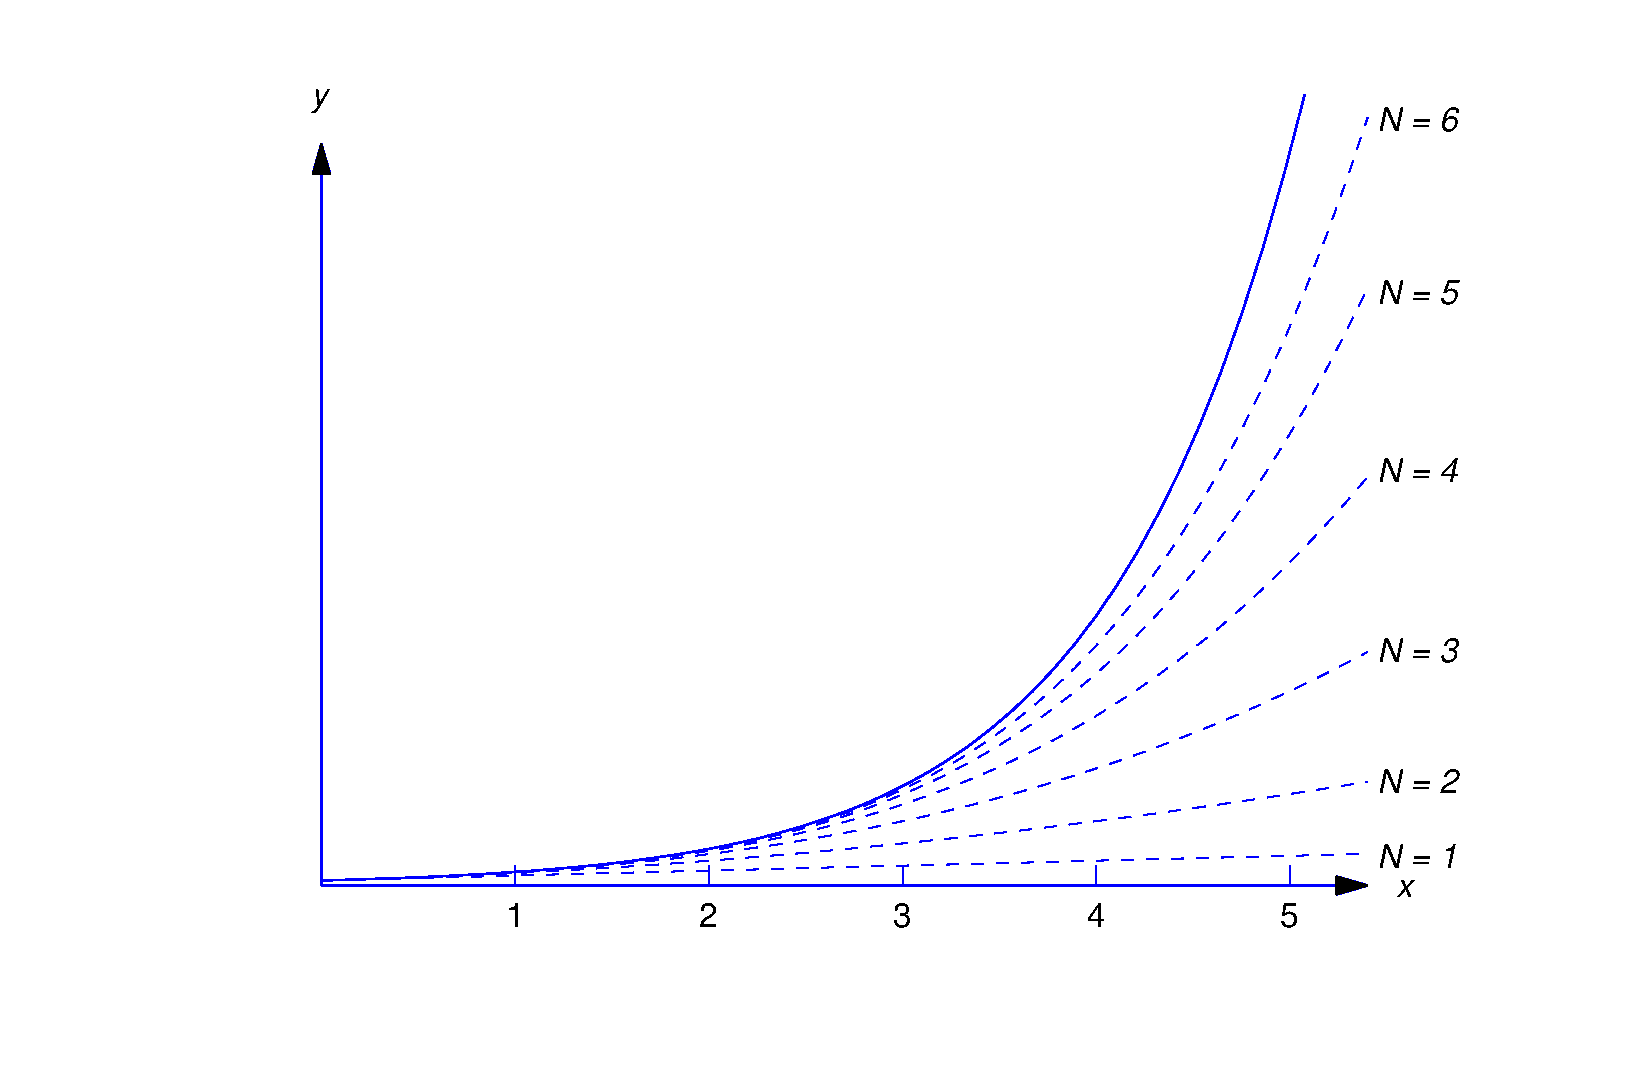
\includegraphics[bb=-78 148 689 643,width=5.67in,height=3.66in,keepaspectratio]{fig070101}
\caption{ Approximation of $y=e^x$ by Taylor
polynomials about $x=0$}
  \label{figure:7.1.1}
\end{figure}

\boxit{Shifting the Summation Index}

\noindent
In Definition~\ref{thmtype:7.1.1} of a power series in $x-x_0$, the $n$-th
term is a constant multiple of $(x-x_0)^n$. This isn't  true in
\eqref{eq:7.1.6}, \eqref{eq:7.1.7}, and \eqref{eq:7.1.8}, where the general
terms are constant multiples of $(x-x_0)^{n-1}$, $(x-x_0)^{n-2}$, and
$(x-x_0)^{n-k}$, respectively. However, these series can all be
rewritten so that their $n$-th terms are constant multiples of
$(x-x_0)^n$. For example, letting $n=k+1$ in the series in
\eqref{eq:7.1.6} yields
\begin{equation} \label{eq:7.1.10}
f'(x)=\sum_{k=0}^\infty (k+1)a_{k+1}(x-x_0)^k,
\end{equation}
where we start the new summation index $k$ from zero so that the first
term in \eqref{eq:7.1.10} (obtained by setting $k=0$) is the same as the
first term in \eqref{eq:7.1.6} (obtained by setting $n=1$). However, the
sum of a series is independent of the symbol used to denote the
summation index, just as the value of a definite integral is
independent of the symbol used to denote the variable of integration.
Therefore we can replace $k$ by $n$ in \eqref{eq:7.1.10} to obtain
\begin{equation} \label{eq:7.1.11}
f'(x)=\sum_{n=0}^\infty (n+1)a_{n+1}(x-x_0)^n,
\end{equation}
where the general term is a  constant multiple of  $(x-x_0)^n$.

It isn't  really necessary to introduce the intermediate summation
index $k$. We can obtain \eqref{eq:7.1.11} directly from \eqref{eq:7.1.6}
by replacing $n$ by $n+1$ in the general term of \eqref{eq:7.1.6} and
subtracting $1$ from the lower limit of \eqref{eq:7.1.6}. More generally,
we use the following procedure for shifting indices.

\bigbox{%\figspace{-25pt}
\begin{center}{\bf Shifting the Summation Index in a Power
Series}\end{center}
For any integer $k$,  the power series
$$
\sum_{n=n_0}^\infty b_n(x-x_0)^{n-k}
$$
can be rewritten  as
$$
\sum_{n=n_0-k}^\infty b_{n+k}(x-x_0)^n;
$$
that is, replacing $n$ by $n+k$ in the general term and subtracting
$k$ from the lower limit of summation leaves the series unchanged.}

\begin{example}\label{example:7.1.3} \rm
Rewrite the following power series from \eqref{eq:7.1.7}  and \eqref{eq:7.1.8}
so that the general term in each  is a  constant multiple of
$(x-x_0)^n$:
$$
\mbox{\bf (a)}\;
\sum_{n=2}^\infty
n(n-1)a_n(x-x_0)^{n-2}\quad \mbox{\bf (b)}\;
\sum_{n=k}^\infty
n(n-1)\cdots(n-k+1)a_n(x-x_0)^{n-k}.
$$
\end{example}

\solutionpart{a}  Replacing $n$ by $n+2$ in the general term
and subtracting $2$ from the lower limit of summation yields
$$
\sum_{n=2}^\infty n(n-1)a_n(x-x_0)^{n-2}=
\sum_{n=0}^\infty (n+2)(n+1)a_{n+2}(x-x_0)^n.
$$

\solutionpart{b}  Replacing $n$ by $n+k$ in the general term
and subtracting $k$ from the lower limit of summation yields
$$
\sum_{n=k}^\infty
n(n-1)\cdots(n-k+1)a_n(x-x_0)^{n-k}=
\sum_{n=0}^\infty (n+k)(n+k-1)\cdots(n+1)a_{n+k}(x-x_0)^n.
$$

\begin{example}\label{example:7.1.4} \rm
Given that
$$
f(x)=\sum_{n=0}^\infty a_nx^n,
$$
write the function $xf''$  as a power series in which the general term
is a  constant multiple of~$x^n$.
\end{example}

\solution
From Theorem~\ref{thmtype:7.1.4} with $x_0=0$,
$$
f''(x)=\sum_{n=2}^\infty n(n-1)a_nx^{n-2}.
$$
Therefore
$$
xf''(x)=\sum_{n=2}^\infty n(n-1)a_nx^{n-1}.
$$
Replacing $n$ by $n+1$ in the general term and  subtracting $1$
from the lower limit of summation yields
$$
xf''(x)=\sum_{n=1}^\infty (n+1)na_{n+1}x^n.
$$
We can also write this as
$$
xf''(x)=\sum_{n=0}^\infty (n+1)na_{n+1}x^n,
$$
since the first term in this last series is zero.  (We'll see
later that  sometimes it's useful to include zero terms at the
beginning of a series.)

\boxit{Linear Combinations of Power Series}

\noindent
If a power series is multiplied by a constant, then the constant can be
placed inside the summation; that is,
$$
c\sum_{n=0}^\infty a_n(x-x_0)^n=\sum_{n=0}^\infty ca_n(x-x_0)^n.
$$
Two power series
$$
f(x)=\sum_{n=0}^\infty a_n(x-x_0)^n\quad\mbox{ and }\quad
g(x)=\sum_{n=0}^\infty b_n(x-x_0)^n
$$
with positive radii of convergence can be added term by term at points
common to their open intervals of convergence;   thus, if the first
series converges for $|x-x_0|<R_1$ and the second converges for
$|x-x_0|<R_2$, then
$$
f(x)+g(x)=\sum_{n=0}^\infty(a_n+b_n)(x-x_0)^n
$$
for $|x-x_0|<R$, where $R$ is the smaller of $R_1$ and $R_2$.
More generally, linear combinations of power series can be formed term
by term;   for example,
$$
c_1f(x)+c_2f(x)=\sum_{n=0}^\infty(c_1a_n+c_2b_n)(x-x_0)^n.
$$

\begin{example}\label{example:7.1.5} \rm
Find the Maclaurin series for $\cosh x$  as a linear
combination of the Maclaurin series for $e^x$ and $e^{-x}$.
\end{example}

\solution
By definition,
$$
\cosh x={1\over2}e^x+{1\over2}e^{-x}.
$$
Since
$$ e^x=\sum_{n=0}^\infty  {x^n\over n!}\quad\mbox{ and }\quad
 e^{-x}=\sum_{n=0}^\infty (-1)^n {x^n\over n!},
$$
it follows that
\begin{equation} \label{eq:7.1.12}
\cosh x=\sum_{n=0}^\infty {1\over2}[1+(-1)^n]{x^n\over n!}.
\end{equation}
Since
$$
{1\over2}[1+(-1)^n]=\left\{\begin{array}{cl}1&\mbox{ if } n=2m,\mbox{
an even integer},\\ 0&\mbox{ if }n=2m+1,\mbox{ an odd integer},
\end{array}\right.
$$
we can rewrite \eqref{eq:7.1.12} more simply as
$$
\cosh x=\sum_{m=0}^\infty{x^{2m}\over(2m)!}.
$$
This result is valid on $(-\infty,\infty)$, since this is the open
interval of convergence of the Maclaurin series for $e^x$ and
$e^{-x}$.

\begin{example}\label{example:7.1.6} \rm
Suppose
$$
y=\sum_{n=0}^\infty a_n x^n
$$
 on an open interval $I$ that contains the origin.
\begin{alist}
\item % (a)
Express
$$
(2-x)y''+2y
$$
as a power series in $x$ on $I$.
\item % (b)
Use the result of \part{a} to find necessary and sufficient conditions
on the coefficients $\{a_n\}$ for
 $y$ to be  a solution of the homogeneous equation
\begin{equation} \label{eq:7.1.13}
(2-x)y''+2y=0
\end{equation}
on $I$.
\end{alist}
\end{example}

\solutionpart{a}
From \eqref{eq:7.1.7} with $x_0=0$,
$$
y''=\sum_{n=2}^\infty n(n-1)a_nx^{n-2}.
$$
Therefore
\begin{equation} \label{eq:7.1.14}
\begin{array}{rcl}
(2-x)y''+2y&=&2y''-xy'+2y\\ [\jot]
&=&\dst{\sum_{n=2}^\infty 2n(n-1)a_nx^{n-2}
-\sum_{n=2}^\infty n(n-1)a_nx^{n-1}
+\sum_{n=0}^\infty 2a_n x^n}.
\end{array}
\end{equation}
To combine the three series we  shift indices in the first two to
make their general terms  constant multiples of $x^n$;   thus,
\begin{equation} \label{eq:7.1.15}
\sum_{n=2}^\infty
2n(n-1)a_nx^{n-2}=\sum_{n=0}^\infty2(n+2)(n+1)a_{n+2}x^n
\end{equation}
and
\begin{equation} \label{eq:7.1.16}
\sum_{n=2}^\infty n(n-1)a_nx^{n-1}=\sum_{n=1}^\infty(n+1)na_{n+1}x^n
=\sum_{n=0}^\infty(n+1)na_{n+1}x^n,
\end{equation}
where we added a zero term in the last series so that when we
substitute from \eqref{eq:7.1.15} and \eqref{eq:7.1.16} into \eqref{eq:7.1.14}
all three series will start with $n=0$;   thus,
\begin{equation} \label{eq:7.1.17}
(2-x)y''+2y=\sum_{n=0}^\infty
[2(n+2)(n+1)a_{n+2}-(n+1)na_{n+1}+2a_n]x^n.
\end{equation}

\solutionpart{b} From   \eqref{eq:7.1.17}
we see that $y$ satisfies \eqref{eq:7.1.13} on $I$ if
\begin{equation} \label{eq:7.1.18}
2(n+2)(n+1)a_{n+2}-(n+1)na_{n+1}+2a_n=0,\quad n=0,1,2, \dots.
\end{equation}
Conversely, Theorem~\ref{thmtype:7.1.6}~\part{b} implies that if
$y=\sum_{n=0}^\infty a_nx^n$
satisfies \eqref{eq:7.1.13} on $I$,  then \eqref{eq:7.1.18} holds.

\begin{example}\label{example:7.1.7} \rm
Suppose
$$
y=\sum_{n=0}^\infty a_n (x-1)^n
$$
 on an open interval $I$ that contains $x_0=1$.
Express the function
\begin{equation} \label{eq:7.1.19}
(1+x)y''+2(x-1)^2y'+3y
\end{equation}
as a power series in $x-1$ on $I$.
\end{example}

\solution  Since we want a  power series in $x-1$,
we rewrite the coefficient of $y''$ in \eqref{eq:7.1.19} as
$1+x=2+(x-1)$, so   \eqref{eq:7.1.19} becomes
$$
2y''+(x-1)y''+2(x-1)^2y'+3y.
$$
From \eqref{eq:7.1.6}  and \eqref{eq:7.1.7} with $x_0=1$,
$$
y'=\sum_{n=1}^\infty na_n(x-1)^{n-1}\quad\mbox{ and }\quad
y ''=\sum_{n=2}^\infty n(n-1)a_n(x-1)^{n-2}.
$$
Therefore
\begin{eqnarray*}
2y ''&=&\sum_{n=2}^\infty 2n(n-1)a_n(x-1)^{n-2},\\
(x-1)y ''&=&\sum_{n=2}^\infty n(n-1)a_n(x-1)^{n-1},\\
2(x-1)^2y'&=&\sum_{n=1}^\infty2na_n(x-1)^{n+1},\\
3y&=&\sum_{n=0}^\infty 3a_n (x-1)^n.
\end{eqnarray*}
Before adding these four series we shift indices in the first three so
that their general terms become constant multiples of $(x-1)^n$. This
yields
\begin{eqnarray}
2y ''&=&\sum_{n=0}^\infty 2(n+2)(n+1)a_{n+2}(x-1)^n,\label{eq:7.1.20}\\
(x-1)y''&=&\sum_{n=0}^\infty (n+1)na_{n+1}(x-1)^n,
\label{eq:7.1.21}\\
2(x-1)^2y'&=&\sum_{n=1}^\infty 2(n-1)a_{n-1}(x-1)^n,\label{eq:7.1.22}\\
%dummy \eqref{eq:7.1.22}
3y&=&\sum_{n=0}^\infty 3a_n (x-1)^n, \label{eq:7.1.23}
\end{eqnarray}
where we added initial zero terms to the series in \eqref{eq:7.1.21}
and \eqref{eq:7.1.22}.  Adding \eqref{eq:7.1.20}--\eqref{eq:7.1.23} yields
\begin{eqnarray*}
(1+x)y''+2(x-1)^2y'+3y&=&2y''+(x-1)y''+2(x-1)^2y'+3y\\[5pt]
&=&\sum_{n=0}^\infty  b_n (x-1)^n,
\end{eqnarray*}
where
\begin{eqnarray}
b_0&=&4a_2+3a_0, \label{eq:7.1.24}\\
b_n&=&2(n+2)(n+1)a_{n+2}+(n+1)na_{n+1}+2(n-1)a_{n-1}+3a_n,\,
n\ge1\label{eq:7.1.25}.
\end{eqnarray}
The formula \eqref{eq:7.1.24} for $b_0$  can't be obtained by
setting $n=0$ in \eqref{eq:7.1.25}, since the summation in \eqref{eq:7.1.22}
begins with $n=1$,  while those in \eqref{eq:7.1.20}, \eqref{eq:7.1.21},
and \eqref{eq:7.1.23} begin with $n=0$.

\exercises
\begin{exerciselist}

\item\label{exer:7.1.1}
For each power series use Theorem~\ref{thmtype:7.1.3} to find the radius
of convergence $R$. If $R>0$, find the open interval of convergence.

\begin{tabular}[t]{@{}p{168pt}@{}p{168pt}}
{\bf (a)} $\dst{\sum_{n=0}^\infty {(-1)^n\over2^nn}(x-1)^n}$&
{\bf (b)} $\dst{\sum_{n=0}^\infty 2^nn(x-2)^n}$\\
{\bf (c)} $\dst{\sum_{n=0}^\infty {n!\over9^n}x^n}$&
{\bf (d)} $\dst{\sum_{n=0}^\infty{n(n+1)\over16^n}(x-2)^n}$\\
{\bf (e)} $\dst{\sum_{n=0}^\infty (-1)^n{7^n\over n!}x^n}$&
{\bf (f)} $\dst{\sum_{n=0}^\infty {3^n\over4^{n+1}(n+1)^2}(x+7)^n}$
\end{tabular}

\item\label{exer:7.1.2}
 Suppose there's an
integer $M$ such that $b_m\ne0$ for $m\ge M$,  and
$$
\lim_{m\to\infty}\left|b_{m+1}\over b_m\right|=L,
$$
where $0\le L\le\infty$. Show that the radius of convergence of
$$
\sum_{m=0}^\infty b_m(x-x_0)^{2m}
$$
is $R=1/\sqrt L$,
which is  interpreted  to mean that $R=0$ if $L=\infty$ or
$R=\infty$ if $L=0$.
\hint{Apply Theorem~$\ref{thmtype:7.1.3}$ to the series $\sum_{m=0}^\infty
b_mz^m$ and then let $z=(x-x_0)^2$.}

\item\label{exer:7.1.3}
For each power series, use the result of Exercise~\ref{exer:7.1.2} to find
the radius of convergence $R$. If $R>0$, find the open interval of
convergence.

\begin{tabular}[t]{@{}p{168pt}@{}p{168pt}}
{\bf (a)} $\dst{\sum_{m=0}^\infty (-1)^m(3m+1)(x-1)^{2m+1}}$&
{\bf (b)} $\dst{\sum_{m=0}^\infty
(-1)^m{m(2m+1)\over2^m}(x+2)^{2m}}$ \\
{\bf (c)} $\dst{\sum_{m=0}^\infty {m!\over(2m)!}(x-1)^{2m}}$&
{\bf (d)} $\dst{\sum_{m=0}^\infty (-1)^m{m!\over9^m}(x+8)^{2m}}$\\
{\bf (e)} $\dst{\sum_{m=0}^\infty(-1)^m{(2m-1)\over3^m}x^{2m+1}}$&
{\bf (f)} $\dst{\sum_{m=0}^\infty(x-1)^{2m}}$
\end{tabular}

\item\label{exer:7.1.4}
Suppose there's an integer $M$ such that $b_m\ne0$ for $m\ge M$,
and
$$
\lim_{m\to\infty}\left|b_{m+1}\over b_m\right|=L,
$$
where $0\le L\le\infty$. Let $k$ be a positive integer. Show that the
radius of convergence of
$$
\sum_{m=0}^\infty b_m(x-x_0)^{km}
$$
is $R=1/\sqrt[k]L$, which is interpreted to mean that $R=0$ if
$L=\infty$ or $R=\infty$ if $L=0$. \hint{Apply
Theorem~$\ref{thmtype:7.1.3}$
to the series $\sum_{m=0}^\infty b_mz^m$ and then let $z=(x-x_0)^k$.}

\item\label{exer:7.1.5}
For each power series use the result of Exercise~\ref{exer:7.1.4} to find
the radius of convergence $R$. If $R>0$, find the open interval of
convergence.

\begin{tabular}[t]{@{}p{168pt}@{}p{168pt}}
{\bf (a)} $\dst{\sum_{m=0}^\infty{(-1)^m\over(27)^m}(x-3)^{3m+2}}$&
{\bf (b)} $\dst{\sum_{m=0}^\infty{x^{7m+6}\over m}}$ \\
{\bf (c)} $\dst{\sum_{m=0}^\infty{9^m(m+1)\over(m+2)}(x-3)^{4m+2}}$&
{\bf (d)} $\dst{\sum_{m=0}^\infty(-1)^m{2^m\over m!}x^{4m+3}}$\\
{\bf (e)} $\dst{\sum_{m=0}^\infty{m!\over(26)^m}(x+1)^{4m+3}}$&
{\bf (f)} $\dst{\sum_{m=0}^\infty{(-1)^m\over8^mm(m+1)}(x-1)^{3m+1}}$
\end{tabular}

\item\label{exer:7.1.6} \Lex
Graph $y=\sin x$ and the Taylor polynomial
$$
T_{2M+1}(x)=\sum_{n=0}^M{(-1)^nx^{2n+1}\over(2n+1)!}
$$
on the interval $(-2\pi,2\pi)$ for $M=1$, $2$, $3$, \dots, until you find
a value of $M$ for which there's no perceptible difference between the
two graphs.

\item\label{exer:7.1.7} \Lex
Graph $y=\cos x$ and the Taylor polynomial
$$
T_{2M}(x)=\sum_{n=0}^M{(-1)^nx^{2n}\over(2n)!}
$$
on the interval $(-2\pi,2\pi)$ for $M=1$, $2$, $3$, \dots, until you find a
value of $M$ for which there's no perceptible difference between the
two graphs.

\item\label{exer:7.1.8} \Lex
Graph $y=1/(1-x)$ and the Taylor polynomial
$$
T_N(x)=\sum_{n=0}^Nx^n
$$
on the interval $[0,.95]$ for $N=1$, $2$, $3$, \dots, until you find a
value of $N$ for which there's no perceptible difference between the
two graphs. Choose the scale on the $y$-axis so that $0\le y\le20$.

\item\label{exer:7.1.9} \Lex
Graph $y=\cosh x$ and the Taylor polynomial
$$
T_{2M}(x)=\sum_{n=0}^M{x^{2n}\over(2n)!}
$$
on the interval $(-5,5)$ for $M=1$, $2$, $3$, \dots, until you find a
value of $M$ for which there's no perceptible difference between the
two graphs.
 Choose the scale on the $y$-axis so that $0\le y\le75$.

\item\label{exer:7.1.10} \Lex
Graph $y=\sinh x$ and the Taylor polynomial
$$
T_{2M+1}(x)=\sum_{n=0}^M{x^{2n+1}\over(2n+1)!}
$$
on the interval $(-5,5)$ for $M=0$, $1$, $2$, \dots, until you find a
value of $M$ for which there's no perceptible difference between the
two graphs.
 Choose the scale on the $y$-axis so that~$-75~\le~y\le~75$.

\exercisetext{In Exercises~\ref{exer:7.1.11}--\ref{exer:7.1.15}
find a power series solution
$y(x)=\sum_{n=0}^\infty a_nx^n$.}

\begin{tabular}[t]{@{}p{168pt}@{}p{168pt}}
\item\label{exer:7.1.11}
$\vspace*{-5pt}(2+x)y''+xy'+3y$&
\item\label{exer:7.1.12}
\vspace*{10pt}$(1+3x^2)y''+3x^2y'-2y$
\end{tabular}

\begin{tabular}[t]{@{}p{168pt}@{}p{168pt}}
\item\label{exer:7.1.13} $(1+2x^2)y''+(2-3x)y'+4y$&
\item\label{exer:7.1.14} $(1+x^2)y''+(2-x)y'+3y$
\end{tabular}

\item\label{exer:7.1.15}
$(1+3x^2)y''-2xy'+4y$

\item\label{exer:7.1.16} Suppose $y(x)=\sum_{n=0}^\infty a_n(x+1)^n$
on an open interval that contains $x_0~=~-1$. Find a power series in
$x+1$ for
$$
xy''+(4+2x)y'+(2+x)y.
$$

\item\label{exer:7.1.17}  Suppose $y(x)=\sum_{n=0}^\infty
a_n(x-2)^n$ on an open interval  that contains $x_0~=~2$.
Find a power series in $x-2$ for
$$
x^2y''+2xy'-3xy.
$$

\item\label{exer:7.1.18}  \Lex
Do the following experiment for various choices of
real numbers  $a_0$ and $a_1$.
\begin{alist}
\item % (a)
Use  differential equations software  to solve the initial
value problem
$$
(2-x)y''+2y=0,\quad y(0)=a_0,\quad y'(0)=a_1,
$$
numerically on $(-1.95,1.95)$. Choose the most accurate method
your software package provides.
(See Section~10.1 for a brief discussion of one such
method.)
\item % (b)
For $N=2$, $3$, $4$, \dots, compute $a_2$, \dots, $a_N$
from Eqn.\eqref{eq:7.1.18} and graph
$$
T_N(x)=\sum_{n=0}^N a_nx^n
$$
and the solution obtained in \part{a} on the same axes.
Continue increasing $N$ until it's obvious that there's
no point in continuing.
(This sounds vague, but you'll know when to stop.)
\end{alist}

\item\label{exer:7.1.19} \Lex
Follow the directions of Exercise~\ref{exer:7.1.18} for the initial
value problem
$$
(1+x)y''+2(x-1)^2y'+3y=0,\quad y(1)=a_0,\quad y'(1)=a_1,
$$
on the interval $(0,2)$. Use Eqns.~\eqref{eq:7.1.24} and \eqref{eq:7.1.25}
to compute $\{a_n\}$.

\item\label{exer:7.1.20}
Suppose the series $\sum_{n=0}^\infty a_nx^n$ converges on an
open interval $(-R,R)$, let $r$ be an arbitrary real number, and
define
$$
y(x)=x^r\sum_{n=0}^\infty a_nx^n=\sum_{n=0}^\infty a_nx^{n+r}
$$
\enlargethispage{1in}
on $(0,R)$. Use Theorem~\ref{thmtype:7.1.4} and the rule for
differentiating the product of two functions to show that
\begin{eqnarray*}
y'(x)&=&\dst{\sum_{n=0}^\infty  (n+r)a_nx^{n+r-1}},\\[10pt]
y''(x)&=&\dst{\sum_{n=0}^\infty(n+r)(n+r-1)a_nx^{n+r-2}},\\
&\vdots&\\
y^{(k)}(x)&=&\dst{\sum_{n=0}^\infty(n+r)(n+r-1)\cdots(n+r-k)a_nx^{n+r-k}}
\end{eqnarray*}
on $(0,R)$
\newpage

\exercisetext{In Exercises~\ref{exer:7.1.21}--\ref{exer:7.1.26} let
$y$ be as defined in Exercise~\ref{exer:7.1.20}, and write the  given
expression in  the form $x^r\sum_{n=0}^\infty b_nx^n$.}

\item\label{exer:7.1.21}
$x^2(1-x)y''+x(4+x)y'+(2-x)y$

\item\label{exer:7.1.22}
$x^2(1+x)y''+x(1+2x)y'-(4+6x)y$

\item\label{exer:7.1.23}
$x^2(1+x)y''-x(1-6x-x^2)y'+(1+6x+x^2)y$

\item\label{exer:7.1.24}
$x^2(1+3x)y''+x(2+12x+x^2)y'+2x(3+x)y$

\item\label{exer:7.1.25}
$x^2(1+2x^2)y''+x(4+2x^2)y'+2(1-x^2)y$

\item\label{exer:7.1.26}
$x^2(2+x^2)y''+2x(5+x^2)y'+2(3-x^2)y$

\end{exerciselist}


\section{Series Solutions Near an Ordinary Point I}

\noindent
Many physical applications give rise to second order homogeneous
linear  differential equations of the form
\begin{equation}\label{eq:7.2.1}
P_0(x)y''+P_1(x)y'+P_2(x)y=0,
\end{equation}
where $P_0$, $P_1$, and $P_2$ are polynomials. Usually the solutions
of these equations can't be expressed in terms of familiar elementary
functions. Therefore we'll consider the problem of representing
solutions of \eqref{eq:7.2.1} with series.

We assume throughout that $P_0$, $P_1$ and $P_2$ have no common
factors. Then we say that $x_0$ is an {\color{blue}\it ordinary point\/} of
\eqref{eq:7.2.1} if $P_0(x_0)\ne0$, or a {\color{blue}\it singular point\/} if
$P_0(x_0)=0$. For  Legendre's equation,
\begin{equation}\label{eq:7.2.2}
(1-x^2)y''-2xy'+\alpha(\alpha+1)y=0,
\end{equation}
$x_0=1$ and $x_0=-1$ are singular points and all other points are
ordinary points. For  Bessel's~ equation,
$$
x^2y''+xy'+(x^2-\nu^2)y=0,
$$
$x_0=0$ is a singular point and all other points are ordinary points.
If $P_0$ is a nonzero constant as in  Airy's
equation,
\begin{equation}\label{eq:7.2.3}
y''-xy=0,
\end{equation}
then every point is an ordinary point.

Since polynomials are continuous everywhere, $P_1/P_0$ and $P_2/P_0$
are continuous at any point $x_0$ that isn't  a zero of $P_0$.
Therefore, if $x_0$ is an ordinary point of \eqref{eq:7.2.1} and $a_0$ and
$a_1$ are arbitrary real numbers, then the initial value problem
\begin{equation}\label{eq:7.2.4}
P_0(x)y''+P_1(x)y'+P_2(x)y=0, \quad  y(x_0)=a_0,\quad y'(x_0)=a_1
\end{equation}
has a unique solution on the largest open interval that contains $x_0$
and does not contain any zeros of $P_0$. To see this, we rewrite the
differential equation in \eqref{eq:7.2.4} as
$$
y''+{P_1(x)\over P_0(x)}y'+{P_2(x)\over P_0(x)}y=0
$$
and apply Theorem~\ref{thmtype:5.1.1} with $p=P_1/P_0$ and $q=P_2/P_0$.
In this section and the next we  consider the problem of
representing  solutions of \eqref{eq:7.2.1}  by power series that
converge  for values of $x$  near an ordinary point $x_0$.

We state the next theorem without proof.

\begin{theorem}\color{blue}\label{thmtype:7.2.1}
Suppose $P_0$, $P_1$, and $P_2$ are polynomials with no common
factor and $P_0$ isn't  identically zero$.$ Let $x_0$ be a point such
that $P_0(x_0)\ne0,$ and let $\rho$ be the distance from $x_0$ to the
nearest zero of $P_0$ in the complex plane. $($If $P_0$ is constant,
then $\rho=\infty$.$)$ Then every solution of
\begin{equation}\label{eq:7.2.5}
P_0(x)y''+P_1(x)y'+P_2(x)y=0
\end{equation}
can be represented by a power series
 \begin{equation}\label{eq:7.2.6}
y=\sum_{n=0}^\infty a_n(x-x_0)^n
\end{equation}
that converges at least on the open interval $(x_0-\rho,x_0+\rho)$.
$($ If $P_0$ is nonconstant$,$ so that $\rho$ is necessarily finite$,$
then the open interval of convergence of $\eqref{eq:7.2.6}$ may be larger
than $(x_0-\rho,x_0+\rho).$ If $P_0$ is constant then $\rho=\infty$
and $(x_0-\rho,x_0+\rho)=(-\infty,\infty)$.$)$
\end{theorem}

We call \eqref{eq:7.2.6} a {\color{blue}\it power series solution in $x-x_0$\/}  of
\eqref{eq:7.2.5}. We'll now develop a method for finding power series
solutions of \eqref{eq:7.2.5}. For this purpose we write \eqref{eq:7.2.5} as
$Ly=0$, where
\begin{equation}\label{eq:7.2.7}
Ly=P_0y''+P_1y'+P_2y.
\end{equation}

Theorem~\ref{thmtype:7.2.1} implies that every solution of $Ly=0$ on
$(x_0-\rho,x_0+\rho)$ can be written as
$$
y=\sum_{n=0}^\infty a_n(x-x_0)^n.
$$
Setting $x=x_0$ in this series and in the series
$$
y'=\sum_{n=1}^\infty na_n(x-x_0)^{n-1}
$$
shows that $y(x_0)=a_0$ and $y'(x_0)=a_1$. Since every initial value
problem \eqref{eq:7.2.4} has a unique solution, this means that $a_0$ and
$a_1$ can be chosen arbitrarily, and  $a_2$, $a_3$, \dots are
uniquely determined by them.

To find $a_2$, $a_3$, \dots, we write $P_0$, $P_1$, and $P_2$ in powers of
$x-x_0$, substitute
$$
y=\sum^\infty_{n=0}a_n(x-x_0)^n,
$$
$$
y'=\sum^\infty_{n=1}na_n(x-x_0)^{n-1},
$$
$$
y''=\sum^\infty_{n=2}n(n-1)a_n(x-x_0)^{n-2}
$$
into \eqref{eq:7.2.7}, and collect the coefficients of like powers of
$x-x_0$. This yields
\begin{equation}\label{eq:7.2.8}
Ly=\sum^\infty_{n=0}b_n(x-x_0)^n,
\end{equation}
where $\{b_0, b_1, \dots, b_n, \dots\}$ are expressed in terms of
$\{a_0, a_1, \dots,a_n, \dots\}$ and the coefficients of $P_0$, $P_1$,
and $P_2$, written in powers of $x-x_0$. Since \eqref{eq:7.2.8} and
\part{a} of Theorem~\ref{thmtype:7.1.6} imply that $Ly=0$ if and only if
$b_n=0$ for $n\ge0$,  all power series solutions in
$x-x_0$ of $Ly=0$ can be obtained by choosing $a_0$ and $a_1$
arbitrarily and computing $a_2$, $a_3$, \dots, successively so that
$b_n=0$
for $n\ge0$. For simplicity, we call the power series obtained  this
way {\color{blue}\it the power series in $x-x_0$ for the general solution\/} of
$Ly=0$, without explicitly identifying the open interval of
convergence of the series.

\begin{example}\label{example:7.2.1}\rm
Let $x_0$ be an arbitrary real number. Find the power series in
$x-x_0$ for the general solution of
\begin{equation}\label{eq:7.2.9}
 y''+ y=0.
\end{equation}
\end{example}

\solution
Here
$$
Ly=y''+y.
$$
If
$$
y=\sum_{n=0}^\infty a_n(x-x_0)^n,
$$
then
$$
y''=\sum_{n=2}^\infty n(n-1)a_n(x-x_0)^{n-2},
$$
so
$$
Ly=\sum_{n=2}^\infty n(n-1)a_n(x-x_0)^{n-2}+\sum_{n=0}^\infty a_n(x-x_0)^n.
$$
To collect coefficients of like powers of $x-x_0$, we shift the summation
index in the first sum. This yields
$$
Ly=\sum^\infty_{n=0}(n+2)(n+1)a_{n+2}(x-x_0)^n +
 \sum^\infty_{n=0}a_n(x-x_0)^n
=\sum^\infty_{n=0}b_n(x-x_0)^n,
$$
with
$$
b_n=(n+2)(n+1)a_{n+2}+a_n.
$$
Therefore $Ly=0$ if and only if
\begin{equation}\label{eq:7.2.10}
a_{n+2}={-a_n\over(n+2)(n+1)},\quad n\ge0,
\end{equation}
where $a_0$ and $a_1$ are arbitrary. Since the indices on the left and
right sides of \eqref{eq:7.2.10} differ by two, we write \eqref{eq:7.2.10}
separately for $n$ even $(n=2m)$ and $n$ odd $(n=2m+1)$. This yields
\begin{eqnarray}
a_{2m+2}&=&{-a_{2m}\over(2m+2)(2m+1)},\quad m\ge0,
\label{eq:7.2.11} \\%dummy \eqref{eq:7.2.14}
\noalign{\hspace*{-15pt}\mbox{and}}\nonumber\\
a_{2m+3}&=&{-a_{2m+1}\over(2m+3)(2m+2)},\quad  m\ge0.
\label{eq:7.2.12}
\end{eqnarray}
Computing the coefficients of the even powers of $x-x_0$ from
\eqref{eq:7.2.11} yields
\begin{eqnarray*}
a_2&=&-{a_0\over2\cdot1}\\[2\jot]
a_4&=&-{a_2\over4\cdot3}=-{1\over4\cdot3}
 \left(-{a_0\over2\cdot1}\right)=
 {a_0\over4\cdot3\cdot2\cdot1}, \\
a_6&=&-{a_4\over6\cdot5}=-{1\over6\cdot5}
 \left({a_0\over4\cdot3\cdot2\cdot1}\right)
=-{a_0\over6\cdot5\cdot4\cdot3\cdot
 2\cdot1},
\end{eqnarray*}
and, in general,
\begin{equation}\label{eq:7.2.13}
a_{2m}=(-1)^m {a_0\over(2m)!}\;   ,\quad  m\ge0.
\end{equation}
Computing the coefficients of the odd powers of $x-x_0$ from \eqref{eq:7.2.12}
yields
\begin{eqnarray*}
a_3&=&-{a_1\over3\cdot2}\\[2\jot]
a_5&=&-{a_3\over5\cdot4}=-{1\over5\cdot4}
 \left(-{a_1\over3\cdot2}\right)=
 {a_1\over5\cdot4\cdot3\cdot2}, \\
a_7&=&-{a_5\over7\cdot6}=-{1\over7\cdot6}
 \left({a_1\over5\cdot4\cdot3\cdot2}\right)
=-{a_1\over7\cdot6\cdot5\cdot4\cdot
 3\cdot2},
\end{eqnarray*}
and, in general,
\begin{equation}\label{eq:7.2.14}
a_{2m+1}={(-1)^ma_1\over(2m+1)!}\quad m\ge0.
\end{equation}
Thus, the general solution of \eqref{eq:7.2.9} can be written as
$$
y=\sum_{m=0}^\infty a_{2m}(x-x_0)^{2m}+\sum_{m=0}^\infty a_{2m+1}(x-x_0)^{2m+1},
$$
or, from \eqref{eq:7.2.13} and \eqref{eq:7.2.14}, as
\begin{equation}\label{eq:7.2.15}
y=a_0\sum_{m=0}^\infty(-1)^m{(x-x_0)^{2m}\over(2m)!}
+a_1\sum_{m=0}^\infty(-1)^m{(x-x_0)^{2m+1}\over(2m+1)!}.
\end{equation}
If we recall from calculus that
$$
\sum_{m=0}^\infty(-1)^m{(x-x_0)^{2m}\over(2m)!}=\cos(x-x_0)
\mbox{\quad  and \quad }
\sum_{m=0}^\infty(-1)^m{(x-x_0)^{2m+1}\over(2m+1)!}=\sin(x-x_0),
$$
then \eqref{eq:7.2.15} becomes
$$
y=a_0\cos(x-x_0)+a_1\sin(x-x_0),
$$
which should look familiar. \bbox

Equations like \eqref{eq:7.2.10}, \eqref{eq:7.2.11}, and \eqref{eq:7.2.12}, which
define a given coefficient in the sequence $\{a_n\}$ in terms of one
or more coefficients with lesser indices are called {\color{blue}\it recurrence
relations\/}. When we use a recurrence relation to compute terms
of a sequence we're computing {\color{blue}\it recursively\/}.

In  the remainder of this  section we  consider the problem of
finding power series solutions in $x-x_0$  for equations of the form
\begin{equation}\label{eq:7.2.16}
\left(1+\alpha(x-x_0)^2\right)y''+\beta(x-x_0) y'+\gamma y=0.
\end{equation}
Many important equations that arise in applications are of this
form with $x_0=0$, including  Legendre's equation \eqref{eq:7.2.2},
Airy's equation \eqref{eq:7.2.3},
\href{https://mathshistory.st-andrews.ac.uk/Biographies/Chebyshev/}
{\color{blue}\it Chebyshev's  equation\/},
$$
(1-x^2)y''-xy'+\alpha^2 y=0,
$$
and
\href{https://mathshistory.st-andrews.ac.uk/Biographies/Hermite/}
{\color{blue}\it Hermite's equation},
$$
y''-2xy'+2\alpha y=0.
$$
Since
$$
P_0(x)=1+\alpha(x-x_0)^2
$$
in \eqref{eq:7.2.16}, the point $x_0$ is an ordinary point of
\eqref{eq:7.2.16}, and Theorem~\ref{thmtype:7.2.1} implies that the solutions
of \eqref{eq:7.2.16} can be written as power series in $x-x_0$ that
converge on the interval $(x_0-1/\sqrt|\alpha|,x_0+1/\sqrt|\alpha|)$
if $\alpha\ne0$, or on $(-\infty,\infty)$ if $\alpha=0$. We'll see
that the coefficients in these power series can be obtained by methods
similar to the one used in Example~\ref{example:7.2.1}.

To simplify
finding the coefficients, we introduce some notation for
products:
$$
\prod^s_{j=r}b_j=b_rb_{r+1}\cdots b_s\quad \mbox{if}
\quad s\ge r.
$$
Thus,
$$
\prod^7_{j=2}b_j=b_2b_3b_4b_5b_6b_7,
$$
$$
\prod^4_{j=0}(2j+1)=(1)(3)(5)(7)(9)=945,
$$
and
$$
\prod^2_{j=2}j^2=2^2=4.
$$
We define
$$
\prod^s_{j=r}b_j=1\quad \mbox{if}\quad s < r,
$$
no matter what the form of $b_j$.

\begin{example}\label{example:7.2.2}\rm
Find the power series in $x$ for the general solution of
\begin{equation}\label{eq:7.2.17}
 (1+2x^2)y''+6xy'+2y=0.
\end{equation}
\end{example}

\solution
Here
$$
Ly=(1+2x^2)y''+6xy'+2y.
$$
If
$$
y=\sum_{n=0}^\infty a_nx^n
$$
then
$$
y'=\sum_{n=1}^\infty na_nx^{n-1}\quad\mbox{ and }\quad
y''=\sum_{n=2}^\infty n(n-1)a_nx^{n-2},
$$
so
\begin{eqnarray*}
Ly&=&(1+2x^2) \sum^\infty_{n=2}n(n-1)a_nx^{n-2}+ 6x
 \sum^\infty_{n=1}na_nx^{n-1}
 +2 \sum^\infty_{n=0}a_nx^n\\[2\jot]
&=&\sum_{n=2}^\infty n(n-1)a_nx^{n-2}+\sum_{n=0}^\infty
\left[2n(n-1)+6n+2\right]a_nx^n\\[2\jot]
&=&\sum_{n=2}^\infty n(n-1)a_nx^{n-2}+2\sum_{n=0}^\infty(n+1)^2a_nx^n.
\end{eqnarray*}
To collect coefficients of $x^n$,  we shift the summation index
in the first sum.  This yields
$$
Ly=\sum_{n=0}^\infty(n+2)(n+1)a_{n+2}x^n+2\sum_{n=0}^\infty(n+1)^2a_nx^n
=\sum_{n=0}^\infty b_nx^n,
$$
with
$$
b_n=(n+2)(n+1)a_{n+2}+2(n+1)^2a_n,\quad n\ge0.
$$
To obtain solutions of \eqref{eq:7.2.17}, we set $b_n=0$ for $n\ge0$. This
is equivalent to the recurrence relation
 \begin{equation}\label{eq:7.2.18}
a_{n+2}=-2{n+1\over n+2}a_n,\quad n\ge0.
\end{equation}
Since the
indices on the left and right differ by two, we write \eqref{eq:7.2.18}
separately for $n=2m$ and $n=2m+1$, as in Example~\ref{example:7.2.1}.
This yields
\begin{eqnarray}
a_{2m+2}&=&-2 {2m+1\over2m+2}a_{2m}=-{2m+1\over m+1}a_{2m},\quad m
\ge0,\label{eq:7.2.19}\\
\noalign{\hspace*{-15pt}\mbox{and}}\nonumber\\
a_{2m+3}&=&-2{2m+2\over2m+3}a_{2m+1}=-4{m+1\over2m+3}a_{2m+1},\quad
m\ge0. \label{eq:7.2.20}
\end{eqnarray}
Computing the coefficients of even powers of $x$ from \eqref{eq:7.2.19}
yields
\begin{eqnarray*}
a_2&=&-{1\over1}a_0,\\[5pt]
a_4&=&-{3\over2}a_2=\left(-{3\over2}\right)\left(-{1\over1}\right)a_0
={1\cdot3\over1\cdot2}a_0,
\\[5pt] a_6&=&-{5\over3}a_4=
-{5\over3}\left(1\cdot3\over1\cdot2\right)a_0
=-{1\cdot3\cdot5\over1\cdot2\cdot3}a_0, \\[5pt]
a_8&=&-{7\over4}a_6=-{7\over4}
\left(-{1\cdot3\cdot5\over1\cdot2\cdot3}\right)a_0=
{1\cdot3\cdot5\cdot7\over1\cdot2\cdot3\cdot4}a_0.\\
\end{eqnarray*}
In general,
\begin{equation}\label{eq:7.2.21}
a_{2m}=(-1)^m{\prod_{j=1}^m(2j-1)\over m!}a_0,\quad m\ge0.
\end{equation}
(Note that \eqref{eq:7.2.21} is correct for $m=0$  because we
defined $\prod_{j=1}^0b_j=1$  for any~$b_j$.)

Computing the coefficients of odd powers of $x$ from \eqref{eq:7.2.20}
yields
\begin{eqnarray*}
a_3&=&-4\,{1\over3}a_1, \\[5pt]
a_5&=&-4\,{2\over5}a_3=-4\,{2\over5}\left(-4{1\over3}\right)a_1
=4^2{1\cdot2\over3\cdot5}a_1,
\\[5pt] a_7&=&-4\,{3\over7}a_5=-4\,{3\over7}\left(
4^2{1\cdot2\over3\cdot5}\right)a_1=
-4^3{1\cdot2\cdot3\over3\cdot5\cdot7}a_1,\\[5pt]
a_9&=&-4\, {4\over9}a_7=-4\, {4\over9}\left(
4^3{1\cdot2\cdot3\over3\cdot5\cdot7}\right)a_1=
4^4{1\cdot2\cdot3\cdot4\over3\cdot5\cdot7\cdot9}a_1.
\end{eqnarray*}
In general,
\begin{equation}\label{eq:7.2.22}
a_{2m+1}={(-1)^m4^m m!\over\prod_{j=1}^m(2j+1)}a_1,\quad m\ge0.
\end{equation}
From \eqref{eq:7.2.21} and \eqref{eq:7.2.22},
$$
y=a_0
 \sum^\infty_{m=0}(-1)^m {\prod_{j=1}^m(2j-1)\over m!}x^{2m}
+a_1 \sum^\infty_{m=0}(-1)^m {4^mm!\over\prod_{j=1}^m(2j+1)}
 x^{2m+1}.
$$
is the power series in $x$ for the general solution of \eqref{eq:7.2.17}.
Since $P_0(x)=1+2x^2$ has no real zeros, Theorem~\ref{thmtype:5.1.1} implies
that every solution of \eqref{eq:7.2.17} is defined on $(-\infty,\infty)$.
However, since $P_0(\pm i/\sqrt2)=0$, Theorem~\ref{thmtype:7.2.1} implies
only that the power series converges in $(-1/\sqrt2,1/\sqrt2)$ for any
choice of $a_0$ and $a_1$.

The results in Examples~\ref{example:7.2.1} and \ref{example:7.2.2} are
consequences of the following general theorem.

\begin{theorem}\color{blue}\label{thmtype:7.2.2}
The coefficients $\{a_n\}$ in any solution
$y=\sum_{n=0}^\infty a_n(x-x_0)^n$ of
\begin{equation}\label{eq:7.2.23}
\left(1+\alpha(x-x_0)^2\right)y''+\beta(x-x_0) y'+\gamma y=0
\end{equation}
satisfy the recurrence relation
\begin{equation}\label{eq:7.2.24}
a_{n+2}=-{p(n) \over(n+2)(n+1)}a_n,\quad  n\ge0,
\end{equation}
where
\begin{equation}\label{eq:7.2.25}
p(n)=\alpha n(n-1) +\beta n+\gamma.
\end{equation}
Moreover$,$ the coefficients of the even and odd powers of $x-x_0$ can
be computed separately as
\begin{eqnarray}
a_{2m+2}&=&-{p(2m)\over(2m+2)(2m+1)}a_{2m},\quad m\ge0\label{eq:7.2.26}\\
\noalign{\hspace*{-15pt}\mbox{and}}\nonumber\\
a_{2m+3}&=&-{p(2m+1)\over(2m+3)(2m+2)}a_{2m+1},\quad m\ge0, \label{eq:7.2.27}
\end{eqnarray}
where $a_0$ and $a_1$ are arbitrary.
\end{theorem}

\proof   Here
$$
Ly=\left(1+\alpha(x-x_0\right)^2)y''+\beta(x-x_0) y'+\gamma y.
$$
If
$$
y=\sum_{n=0}^\infty a_n(x-x_0)^n,
$$
then
$$
y'=\sum_{n=1}^\infty na_n(x-x_0)^{n-1}
\quad\mbox{ and }\quad y''=\sum_{n=2}^\infty n(n-1)a_n(x-x_0)^{n-2}.
$$
Hence,
$$
\begin{array}{ccl}
Ly&=&\dst{\sum_{n=2}^\infty n(n-1)a_n(x-x_0)^{n-2}+
\sum_{n=0}^\infty \left[\alpha
n(n-1)
+\beta n+\gamma\right]a_n(x-x_0)^n}\\[2\jot]
&=&\dst{\sum_{n=2}^\infty n(n-1)a_n(x-x_0)^{n-2}+\sum_{n=0}^\infty
p(n)a_n(x-x_0)^n},
\end{array}
$$
from \eqref{eq:7.2.25}.  To collect coefficients of powers of $x-x_0$,
we shift the summation index in the first sum. This yields
$$
Ly=\sum_{n=0}^\infty \left[(n+2)(n+1)a_{n+2}+p(n)a_n\right](x-x_0)^n.
$$
Thus, $Ly=0$ if and only if
$$
(n+2)(n+1)a_{n+2}+p(n)a_n=0,\quad n\ge0,
$$
which is equivalent to \eqref{eq:7.2.24}. Writing \eqref{eq:7.2.24} separately
for the cases where $n=2m$ and $n=2m+1$ yields \eqref{eq:7.2.26} and
\eqref{eq:7.2.27}.

\begin{example}\label{example:7.2.3}\rm
Find the power series in $x-1$  for the general
solution of
\begin{equation}\label{eq:7.2.28}
(2+4x-2x^2)y''-12(x-1)y'-12y=0.
\end{equation}
\end{example}

\solution
We must first write the coefficient $P_0(x)=2+4x-x^2$ in powers of
$x-1$. To do this,
 we write $x=(x-1)+1$ in $P_0(x)$ and then expand
the terms, collecting powers of $x-1$;   thus,
\begin{eqnarray*}
2+4x-2x^2&=&2+4[(x-1)+1]-2[(x-1)+1]^2\\
&=&4-2(x-1)^2.
\end{eqnarray*}
  Therefore we can rewrite \eqref{eq:7.2.28} as
$$
\left(4-2(x-1)^2\right)y''-12(x-1)y'-12y=0,
$$
or, equivalently,
$$
\left(1-{1\over2}(x-1)^2\right)y''-3(x-1)y'-3y=0.
$$
This is of the form \eqref{eq:7.2.23} with  $\alpha=-1/2$, $\beta=-3$, and
$\gamma=-3$. Therefore, from \eqref{eq:7.2.25}
$$
p(n)=-{n(n-1)\over2}-3n-3=-{(n+2)(n+3)\over2}.
$$
Hence, Theorem~\ref{thmtype:7.2.2} implies that
\begin{eqnarray*}
a_{2m+2}&=&-{p(2m)\over(2m+2)(2m+1)}a_{2m}\\[2\jot]&=&
{(2m+2)(2m+3)\over2(2m+2)(2m+1)}
a_{2m}={2m+3\over2(2m+1)}a_{2m},\quad m\ge0\\
\noalign{\hspace*{-15pt}\mbox{and}}\\
a_{2m+3}&=&-{p(2m+1)\over(2m+3)(2m+2)}a_{2m+1}\\[2\jot]&=&
{(2m+3)(2m+4)\over2
(2m+3)(2m+2)}a_{2m+1}={m+2\over2(m+1)}a_{2m+1},\quad m\ge0.
\end{eqnarray*}
We leave it to you to show that
$$
a_{2m}={2m+1\over2^m}a_0\quad\mbox{ and }\quad
a_{2m+1}={m+1\over2^m}a_1,\quad m\ge0,
$$
which implies that the power series in $x-1$ for the general solution
of
\eqref{eq:7.2.28} is
$$
y=a_0\sum_{m=0}^\infty{2m+1\over2^m}(x-1)^{2m}+a_1\sum_{m=0}^\infty
{m+1\over2^m}(x-1)^{2m+1}.\bbox
$$

In the examples considered so far we were able to obtain closed
formulas for coefficients in the power series solutions. In some cases
this is impossible, and we must settle for computing a finite number
of terms in the series. The next example illustrates this with an
initial value problem.

\begin{example}\label{example:7.2.4}\rm
Compute  $a_0$, $a_1$, \dots, $a_7$  in the series solution
$y=\sum_{n=0}^\infty a_nx^n$ of the initial value problem
\begin{equation}\label{eq:7.2.29}
(1+2x^2)y''+10xy'+8y=0,\quad y(0)=2,\quad y'(0)=-3.
\end{equation}
\end{example}

\solution
Since $\alpha=2$, $\beta=10$, and $\gamma=8$ in \eqref{eq:7.2.29},
$$
p(n)=2n(n-1)+10n+8=2(n+2)^2.
$$
 Therefore
$$
a_{n+2}=-2{(n+2)^2\over(n+2)(n+1)}a_n=-2{n+2\over n+1}a_n,\quad n\ge0.
$$
Writing this equation separately for $n=2m$  and $n=2m+1$ yields
\begin{eqnarray}
a_{2m+2}&=&-2{(2m+2)\over2m+1}a_{2m}=-4{m+1\over2m+1}a_{2m},\quad m\ge
0\label{eq:7.2.30}\\
\noalign{\hspace*{-15pt}\mbox{and}}\nonumber\\
a_{2m+3}&=&-2{2m+3\over2m+2}a_{2m+1}=-{2m+3\over m+1}a_{2m+1},\quad m\ge0.
\label{eq:7.2.31}
\end{eqnarray}
Starting with  $a_0=y(0)=2$, we compute $a_2, a_4$, and $a_6$ from
\eqref{eq:7.2.30}:
\begin{eqnarray*}
a_2&=&-4\,{1\over1}2=-8,\\[2\jot]
a_4&=&-4\,{2\over3}(-8)={64\over3},\\[2\jot]
a_6&=&-4\,{3\over5}\left(64\over3\right)=-{256\over5}.
\end{eqnarray*}
Starting with $a_1=y'(0)=-3$, we compute $a_3,a_5$ and $a_7$ from
\eqref{eq:7.2.31}:
\begin{eqnarray*}
a_3&=&-{3\over1}(-3)=9,\\[2\jot]
a_5&=&-{5\over2}9=-{45\over2},\\[2\jot]
a_7&=&-{7\over3}\left(-{45\over2}\right)={105\over2}.
\end{eqnarray*}
Therefore the solution of \eqref{eq:7.2.29} is
$$
y=2-3x-8x^2+9x^3+{64\over3}x^4-{45\over2}x^5-{256\over5}
x^6+{105\over2}x^7+\cdots\; .
$$

\technology
\medskip

Computing coefficients recursively as in Example~\ref{example:7.2.4} is
tedious. We recommend that you do this kind of computation by writing
a short program to implement the appropriate recurrence relation on a
calculator or computer. You may wish to do this in
verifying examples and doing exercises (identified by the
symbol
\Cex) in this chapter that call for numerical computation of the
coefficients in series solutions. We obtained the answers to these
exercises by using software that can produce answers in the form of
rational numbers. However, it's perfectly acceptable - and more
practical - to get your answers in decimal form. You can always check
them by converting our fractions to decimals.

If you're interested in actually using series to compute numerical
approximations to solutions of a differential equation, then whether
or not there's a simple closed form for the coefficients is
essentially irrelevant. For computational purposes it's usually
more efficient to start with the given coefficients $a_0=y(x_0)$ and
$a_1=y'(x_0)$, compute $a_2$, \dots, $a_N$ recursively,
 and then compute approximate values of the solution from the
Taylor polynomial
$$
T_N(x)=\sum_{n=0}^Na_n(x-x_0)^n.
$$
The trick is to decide how to choose $N$ so the approximation
$y(x)\approx T_N(x)$ is sufficiently accurate on the subinterval of
the interval of convergence that you're interested in. In the
computational exercises in this  and the next two sections,
you will often be asked to obtain the solution of a given problem by
numerical integration with  software  of your choice (see
Section~10.1 for a brief discussion of one such method),
and to compare the solution obtained in this way with the
approximations obtained with $T_N$ for various values of $N$. This is
a typical textbook kind of exercise, designed to give you insight into
how the accuracy of the approximation $y(x)\approx T_N(x)$ behaves as
a function of $N$ and the interval that you're working on. In real
life, you would choose one or the other of the two methods (numerical
integration or series solution). If you choose the method of series
solution, then a practical procedure for determining a suitable value
of $N$ is to continue increasing $N$ until the maximum of
$|T_N-T_{N-1}|$ on the interval of interest is within the margin of
error that you're willing to accept.

In doing computational problems  that call for
numerical solution of differential equations you should
choose the most accurate numerical integration procedure  your
software  supports, and experiment with the step size until
you're confident that the numerical results are sufficiently
accurate for the problem at hand.

\exercises
 In Exercises~\ref{exer:7.2.1} --\ref{exer:7.2.8}  find the power
series in $x$ for the general solution.

\begin{exerciselist}
\begin{tabular}[t]{@{}p{168pt}@{}p{168pt}}
\item\label{exer:7.2.1}  $(1+x^2)y''+6xy'+6y=0$&
\vspace*{10pt}\item\label{exer:7.2.2}  $(1+x^2)y''+2xy'-2y=0$
\end{tabular}

\begin{tabular}[t]{@{}p{168pt}@{}p{168pt}}
\item\label{exer:7.2.3}  $(1+x^2)y''-8xy'+20y=0$&
\item\label{exer:7.2.4} $(1-x^2)y''-8xy'-12y=0$
\end{tabular}

\begin{tabular}[t]{@{}p{168pt}@{}p{168pt}}
\item\label{exer:7.2.5} $(1+2x^2)y''+7xy'+2y=0$&
\item\label{exer:7.2.6} $\dst{(1+x^2)y''+2xy'+{1\over4}y=0}$
\end{tabular}

\vspace{-10pt}
\begin{tabular}[t]{@{}p{168pt}@{}p{168pt}}
\item\label{exer:7.2.7} $(1-x^2)y''-5xy'-4y=0$&
\item\label{exer:7.2.8} $(1+x^2)y''-10xy'+28y=0$
\end{tabular}

\newpage

\item\label{exer:7.2.9}  \Lex
\begin{alist}
\item % (a)
Find the power series in $x$ for the general solution of
$y''+xy'+2y=0$.
\item % (b)
For several choices of $a_0$ and $a_1$,
use  differential equations software to solve the initial
value problem
$$
y''+xy'+2y=0,\quad y(0)=a_0,\quad y'(0)=a_1,
\eqno{\rm(A)}
$$
numerically on $(-5,5)$.
\item % ()
For fixed $r$ in $\{1,2,3,4,5\}$ graph
$$
T_N(x)=\sum_{n=0}^N a_nx^n
$$
and the solution obtained in \part{a} on $(-r,r)$.
Continue increasing $N$ until there's no perceptible
difference between the two graphs.
\end{alist}

\item\label{exer:7.2.10}  \Lex
Follow the directions of Exercise~\ref{exer:7.2.9}  for the differential
equation
$$
y''+2xy'+3y=0.
$$

\exercisetext{In Exercises~\ref{exer:7.2.11} --\ref{exer:7.2.13}
 find $a_0$, \dots, $a_N$ for $N$ at least $7$ in the power series
solution
$y=\sum_{n=0}^\infty a_nx^n$
of the initial value problem.}

\item\label{exer:7.2.11} \Cex  $(1+x^2)y''+xy'+y=0,\quad y(0)=2,\quad
y'(0)=-1$
\item\label{exer:7.2.12} \Cex  $(1+2x^2)y''-9xy'-6y=0,\quad y(0)=1,\quad
y'(0)=-1$
\item\label{exer:7.2.13}  \Cex  $(1+8x^2)y''+2y=0,\quad y(0)=2,\quad
y'(0)=-1$

\item\label{exer:7.2.14}   \Lex
Do the next experiment for various choices of
real numbers  $a_0$, $a_1$, and $r$, with $0<r<1/\sqrt2$.
\begin{alist}
\item % (a)
Use  differential equations software  to solve the initial
value problem
$$
(1-2x^2)y''-xy'+3y=0,\quad y(0)=a_0,\quad y'(0)=a_1,
\eqno{\rm(A)}
$$
numerically on $(-r,r)$.
\item % (b)
For $N=2$, $3$, $4$, \dots, compute $a_2$, \dots, $a_N$ in the power series
solution
$y=\sum_{n=0}^\infty a_nx^n$ of (A), and graph
$$
T_N(x)=\sum_{n=0}^N a_nx^n
$$
and the solution obtained in \part{a} on $(-r,r)$.
Continue increasing $N$ until there's no perceptible
difference between the two graphs.
\end{alist}

\item\label{exer:7.2.15}   \Lex
Do \part{a} and \part{b}  for several values of
$r$ in
$(0,1)$:
\begin{alist}
\item % (a)
Use  differential equations software  to solve the initial
value problem
$$
(1+x^2)y''+10xy'+14y=0,\quad y(0)=5,\quad y'(0)=1,
\eqno{\rm(A)}
$$
numerically on $(-r,r)$.
\item % (b)
For $N=2$, $3$, $4$, \dots, compute $a_2$, \dots, $a_N$ in the power series
solution
$y=\sum_{n=0}^\infty a_nx^n$ of (A) , and
graph
$$
T_N(x)=\sum_{n=0}^N a_nx^n
$$
\enlargethispage{1in}
and the solution obtained in \part{a} on $(-r,r)$.
Continue increasing $N$ until there's no perceptible
difference between the two graphs. What  happens to the required $N$
as $r\to1$?
\item % (c)
Try \part{a} and \part{b} with $r=1.2$. Explain your results.
\end{alist}

\newpage

\exercisetext{In Exercises~\ref{exer:7.2.16} --\ref{exer:7.2.20}
 find the power series in $x-x_0$
for the general solution.}

\begin{tabular}[t]{@{}p{120pt}@{}p{130pt}}
\item\label{exer:7.2.16} $y''-y=0;\quad   x_0=3$&\vspace*{5pt}
\vspace*{5pt}\item\label{exer:7.2.17} $y''-(x-3)y'-y=0;\quad   x_0=3$
\end{tabular}

\item\label{exer:7.2.18} $(1-4x+2x^2)y''+10(x-1)y'+6y=0;\quad  x_0=1$
\item\label{exer:7.2.19} $(11-8x+2x^2)y''-16(x-2)y'+36y=0;\quad  x_0=2$
\item\label{exer:7.2.20} $(5+6x+3x^2)y''+9(x+1)y'+3y=0;\quad  x_0=-1$

\exercisetext{In Exercises~\ref{exer:7.2.21} --\ref{exer:7.2.26}
 find $a_0$, \dots, $a_N$ for $N$ at least $7$ in the power series
$y=\sum_{n=0}^\infty a_n(x-x_0)^n$
 for the  solution of the initial value problem.  Take $x_0$ to be the
point where the initial conditions are imposed.}

\item\label{exer:7.2.21}  \Cex $(x^2-4)y''-xy'-3y=0,\quad y(0)=-1,\quad
y'(0)=2$
\item\label{exer:7.2.22}  \Cex $y''+(x-3)y'+3y=0,\quad y(3)=-2,\quad
y'(3)=3$
\item\label{exer:7.2.23}  \Cex $(5-6x+3x^2)y''+(x-1)y'+12y=0,\quad
y(1)=-1,\quad y'(1)=1$
\item\label{exer:7.2.24}  \Cex $(4x^2-24x+37)y''+y=0,\quad y(3)=4,\quad
y'(3)=-6$
\item\label{exer:7.2.25}  \Cex $(x^2-8x+14)y''-8(x-4)y'+20y=0,\quad
y(4)=3,\quad y'(4)=-4$
\item\label{exer:7.2.26}  \Cex
$(2x^2+4x+5)y''-20(x+1)y'+60y=0,\quad y(-1)=3,\quad y'(-1)=-3$

\item\label{exer:7.2.27}
\begin{alist}
\item % (a)
Find a power series in $x$ for the general solution of
$$
(1+x^2)y''+4xy'+2y=0.
\eqno{\rm (A)}
$$
\item % (b)
Use (a) and the formula
$$
{1\over1-r}=1+r+r^2+\cdots+r^n+\cdots \quad(-1<r<1)
$$
for the sum of a geometric series to find a closed form expression for
the general solution of (A) on $(-1,1)$.
\item % (c)
Show that the expression obtained in \part{b} is actually the general
solution of (A) on $(-\infty,\infty)$.
\end{alist}

\item\label{exer:7.2.28}
Use Theorem~\ref{thmtype:7.2.2} to show that the power series in
$x$ for the general solution of
$$
(1+\alpha x^2)y''+\beta xy'+\gamma y=0
$$
is
$$
y=a_0\sum^\infty_{m=0}(-1)^m \left[\prod^{m-1}_{j=0}
p(2j)\right] {x^{2m}\over(2m)!} +
a_1\sum^\infty_{m=0}(-1)^m
\left[\prod^{m-1}_{j=0}p(2j+1)\right]
{x^{2m+1}\over(2m+1)!}.
$$

\item\label{exer:7.2.29}
Use Exercise~\ref{exer:7.2.28}  to
 show that  all  solutions of
$$
(1+\alpha x^2)y''+\beta xy'+\gamma y=0
$$
 are polynomials if and only if
$$
\alpha n(n-1)+\beta n+\gamma=\alpha(n-2r)(n-2s-1),
$$
where $r$ and $s$ are nonnegative integers.
\newpage

\item\label{exer:7.2.30}
\begin{alist}
\item % (a)
Use Exercise~\ref{exer:7.2.28}  to show that the power series in $x$
for the general solution of
$$
(1-x^2)y''-2bxy'+\alpha(\alpha+2b-1)y=0
$$
is $y=a_0y_1+a_1y_2$, where
\begin{eqnarray*}
y_1&=&\sum_{m=0}^\infty \left[\prod_{j=0}^{m-1}(2j-\alpha)(2j+\alpha+2b-1)
\right]{x^{2m}\over(2m)!}\\
\noalign{\hspace*{50pt}\mbox{and}}\\
y_2&=&\sum_{m=0}^\infty \left[\prod_{j=0}^{m-1}(2j+1-\alpha)(2j+\alpha+2b)
\right]{x^{2m+1}\over(2m+1)!}.
\end{eqnarray*}
\item % (b)
Suppose $2b$ isn't  a negative odd integer and $k$ is a
nonnegative integer. Show that $y_1$ is a polynomial of degree $2k$
such that $y_1(-x)=y_1(x)$ if $\alpha=2k$, while $y_2$ is a polynomial
of degree $2k+1$ such that $y_2(-x)=-y_2(-x)$ if $\alpha=2k+1$.
Conclude that if $n$ is a nonnegative integer, then there's a
polynomial $P_n$ of degree $n$ such that $P_n(-x)=(-1)^nP_n(x)$ and
$$
(1-x^2)P_n''-2bxP_n'+n(n+2b-1)P_n=0.
\eqno{\rm (A)}
$$
\item % (c)
Show that (A) implies that
$$
[(1-x^2)^b P_n']'=-n(n+2b-1)(1-x^2)^{b-1}P_n,
$$
and use this to show that if $m$ and $n$ are nonnegative integers, then
$$
\begin{array}{ll}
[(1-x^2)^bP_n']'P_m-[(1-x^2)^bP_m']'P_n=&\\[2\jot]
\hspace*{40pt}\left[m(m+2b-1)-n(n+2b-1)\right](1-x^2)^{b-1}P_mP_n.&
\end{array}
\eqno{\rm (B)}
$$
\item % (d)
Now suppose   $b>0$.
Use (B) and integration by parts to show that
if $m\ne n$, then
$$
\int_{-1}^1 (1-x^2)^{b-1}P_m(x)P_n(x)\,dx=0.
$$
(We say  that $P_m$ and $P_n$ are {\color{blue}\it orthogonal on\/}
$(-1,1)$ {\color{blue}\it with respect to the weighting
function\/}\newline $(1-x^2)^{b-1}$.)
\end{alist}

\item\label{exer:7.2.31}
\begin{alist}
\item % (a)
Use Exercise~\ref{exer:7.2.28}  to show that the power series in $x$
for the general solution
 of Hermite's equation
$$
y''-2xy'+2\alpha y=0
$$
is $y=a_0y_1+a_1y_1$, where
\begin{eqnarray*}
y_1&=&\sum_{m=0}^\infty \left[\prod_{j=0}^{m-1}(2j-\alpha)
\right]{2^mx^{2m}\over(2m)!}\\
\noalign{\hspace*{25pt}\mbox{and}}\\
y_2&=&\sum_{m=0}^\infty \left[\prod_{j=0}^{m-1}(2j+1-\alpha)
\right]{2^mx^{2m+1}\over(2m+1)!}.
\end{eqnarray*}
\item % (b)
Suppose $k$ is a nonnegative integer. Show that $y_1$ is a
polynomial of degree $2k$ such that $y_1(-x)=y_1(x)$ if $\alpha=2k$,
while $y_2$ is a polynomial of degree $2k+1$ such that
$y_2(-x)=-y_2(-x)$ if $\alpha=2k+1$. Conclude that if $n$ is a
nonnegative integer then there's a polynomial $P_n$ of degree $n$
such that $P_n(-x)=(-1)^nP_n(x)$ and
$$
P_n''-2xP_n'+2nP_n=0.
\eqno{\rm (A)}
$$
\item % (c)
Show that (A) implies that
$$
[e^{-x^2}P_n']'=-2ne^{-x^2}P_n,
$$
and use this to show that if $m$ and $n$ are nonnegative integers, then
$$
[e^{-x^2}P_n']'P_m-[e^{-x^2}P_m']'P_n=
2(m-n)e^{-x^2}P_mP_n.
\eqno{\rm (B)}
$$
\item % (d)
Use (B) and integration by parts to show that
if $m\ne n$, then
$$
\int_{-\infty}^\infty e^{-x^2}P_m(x)P_n(x)\,dx=0.
$$
(We say  that $P_m$ and $P_n$ are {\color{blue}\it orthogonal on\/}
$(-\infty,\infty)$ {\color{blue}\it with respect to the weighting function\/}
$e^{-x^2}$.)
\end{alist}

\item\label{exer:7.2.32}
Consider the equation
$$
\left(1+\alpha x^3\right)y''+\beta x^2y'+\gamma xy=0,
\eqno{\rm (A)}
$$
and let
$p(n)=\alpha n(n-1)+\beta n+\gamma$.
(The special case $y''-xy=0$ of (A) is
 Airy's equation.)

\begin{alist}
\item % (a)
 Modify the argument used to prove Theorem~\ref{thmtype:7.2.2}
to show that
$$
y=\sum_{n=0}^\infty a_nx^n
$$
  is a solution of
(A)  if and only if  $a_2=0$  and
$$
a_{n+3}=-{p(n)\over(n+3)(n+2)}a_n,\quad n\ge0.
$$
\item % (b)
Show from (a)  that $a_n=0$  unless $n=3m$  or $n=3m+1$
for some nonnegative integer $m$, and that
\begin{eqnarray*}
a_{3m+3}&=&-{p(3m)\over(3m+3)(3m+2)}a_{3m},\quad m\ge
0,\\
\noalign{\hspace*{50pt}\mbox{and}}\\
a_{3m+4}&=&-{p(3m+1)\over(3m+4)(3m+3)}
a_{3m+1},\quad m\ge0,
\end{eqnarray*}
where $a_0$ and $a_1$ may be specified arbitrarily.
\item % (c)
Conclude from \part{b}  that the  power series in $x$ for the general
solution
of (A)  is
$$
\begin{array}{l}
y=\dst{a_0\sum^\infty_{m=0}(-1)^m \left[\prod^{m-1}_{j=0}
{p(3j)\over3j+2}\right] {x^{3m}\over3^m m!}}\\[2\jot]
\qquad\dst{+a_1\sum^\infty_{m=0}(-1)^m
\left[\prod^{m-1}_{j=0}{p(3j+1)\over3j+4}\right]
{x^{3m+1}\over3^mm!}}.
\end{array}
$$
\end{alist}

\exercisetext{In Exercises~\ref{exer:7.2.33} --\ref{exer:7.2.37}  use the method of
Exercise~\ref{exer:7.2.32}  to find the power series in
$x$ for the general solution.}

\begin{tabular}[t]{@{}p{100pt}@{}p{168pt}}
\item\label{exer:7.2.33} $y''-xy=0$&
\vspace*{10pt}\item\label{exer:7.2.34} $(1-2x^3)y''-10x^2y'-8xy=0$
\end{tabular}

\vspace*{-10pt}
\begin{tabular}[t]{@{}p{168pt}@{}p{168pt}}
\item\label{exer:7.2.35} $(1+x^3)y''+7x^2y'+9xy=0$&
\item\label{exer:7.2.36} $(1-2x^3)y''+6x^2y'+24xy=0$
\end{tabular}

 \item\label{exer:7.2.37} $(1-x^3)y''+15x^2y'-63xy=0$

\item\label{exer:7.2.38}
Consider the equation
$$
\left(1+\alpha x^{k+2}\right)y''+\beta x^{k+1}y'+\gamma x^ky=0,
\eqno{\rm (A)}
$$
where $k$ is a positive integer,
and let
$p(n)=\alpha n(n-1)+\beta n+\gamma$.
\begin{alist}
\item % (a)
Modify the argument used to prove Theorem~\ref{thmtype:7.2.2} to show that
$$
y=\sum_{n=0}^\infty a_nx^n
$$
  is a solution of
(A)  if and only if  $a_n=0$ for $2\le n\le k+1$ and
$$
a_{n+k+2}=-{p(n)\over(n+k+2)(n+k+1)}a_n,\quad n\ge0.
$$
\item % (b)
Show from \part{a}  that $a_n=0$  unless $n=(k+2)m$  or $n=(k+2)m+1$
for some nonnegative integer $m$, and that
\begin{eqnarray*}
a_{(k+2)(m+1)}&=&-{p\left((k+2)m\right)\over
(k+2)(m+1)[(k+2)(m+1)-1]}a_{(k+2)m},\quad m\ge
0, \\
\noalign{\hspace*{50pt}\mbox{and}}\\
a_{(k+2)(m+1)+1}&=&-{p\left((k+2)m+1\right)\over[(k+2)(m+1)+1](k+2)(m+1)}
a_{(k+2)m+1},\quad m\ge0,
\end{eqnarray*}
where $a_0$ and $a_1$ may be specified arbitrarily.
\item % (c)
Conclude from \part{b}  that the  power series in $x$ for the general
solution
of (A) is
$$
\begin{array}{l}
y=a_0\dst{\sum^\infty_{m=0}(-1)^m \left[\prod^{m-1}_{j=0}
{p\left((k+2)j\right)\over(k+2)(j+1)-1}\right] {x^{(k+2)m}\over(k+2)^m
m!}}\\ [15pt]
\qquad+a_1\dst{\sum^\infty_{m=0}(-1)^m
\left[\prod^{m-1}_{j=0}{p\left((k+2)j+1\right)\over(k+2)(j+1)+1}\right]
{x^{(k+2)m+1}\over(k+2)^mm!}}.
\end{array}
$$
\end{alist}

\exercisetext{In Exercises~\ref{exer:7.2.39} --\ref{exer:7.2.44}  use the method of
Exercise~\ref{exer:7.2.38}  to find the power series in $x$
 for the general solution.}

\item\label{exer:7.2.39} $(1+2x^5)y''+14x^4y'+10x^3y=0$

\vspace*{-10pt}
\begin{tabular}[t]{@{}p{100pt}@{}p{168pt}}
\item\label{exer:7.2.40} $y''+x^2y=0$&
\item\label{exer:7.2.41}  $y''+x^6y'+7x^5y=0$
\end{tabular}

\item\label{exer:7.2.42} $(1+x^8)y''-16x^7y'+72x^6y=0$
\item\label{exer:7.2.43} $(1-x^6)y''-12x^5y'-30x^4y=0$
\item\label{exer:7.2.44} $y''+x^5y'+6x^4y=0$

\end{exerciselist}


\section{Series Solutions Near an Ordinary Point II}

\noindent
In this section we continue to find series solutions
$$
y=\sum_{n=0}^\infty a_n(x-x_0)^n
$$
of  initial value problems
\begin{equation} \label{eq:7.3.1}
P_0(x)y''+P_1(x)y'+P_2(x)y=0,\quad y(x_0)=a_0,\quad y'(x_0)=a_1,
\end{equation}
where $P_0$, $P_1$, and $P_2$ are polynomials and $P_0(x_0)\ne0$,
so $x_0$ is an ordinary point of \eqref{eq:7.3.1}.  However, here we
consider  cases where the differential equation in \eqref{eq:7.3.1}
is not of the form
$$
\left(1+\alpha(x-x_0)^2\right)y''+\beta(x-x_0) y'+\gamma y=0,
$$
so Theorem~\ref{thmtype:7.2.2} does not apply, and the computation of the
coefficients $\{a_n\}$ is more complicated. For the equations
considered here it's difficult or impossible to obtain an explicit
formula for $a_n$ in terms of $n$. Nevertheless, we can calculate as
many coefficients as we wish. The next three examples illustrate
this.

\begin{example}\label{example:7.3.1} \rm
Find the coefficients $a_0$, \dots, $a_7$ in the  series solution
$y=\sum^\infty_{n=0}
a_nx^n$  of the initial value problem
\begin{equation} \label{eq:7.3.2}
(1+x+2x^2)y''+(1+7x)y'+2y=0,\quad y(0)=-1,\quad y'(0)=-2.
\end{equation}
\end{example}

\solution
Here
$$
Ly=(1+x+2x^2)y''+(1+7x)y'+2y.
$$
The zeros $(-1\pm i\sqrt7)/4$ of $P_0(x)=1+x+2x^2$ have absolute value
$1/\sqrt2$, so Theorem~\ref{thmtype:7.2.2} implies that the series
solution
converges to the solution of \eqref{eq:7.3.2} on $(-1/\sqrt2,1/\sqrt2)$.
Since
$$
y=\sum^\infty_{n=0} a_nx^n,\quad y'=\sum^\infty_{n=1} n
a_nx^{n-1}\quad\mbox{ and }\quad  y''=\sum^\infty_{n=2}n(n-1)a_nx^{n-2},
$$
\begin{eqnarray*}
Ly&=&\sum^\infty_{n=2}n(n-1)a_nx^{n-2}+\sum^\infty_{n=2}n(n-1)a_nx^{n-1}
+2\sum^\infty_{n=2}n(n-1)a_nx^n\\[10pt]
&&+\sum^\infty_{n=1}na_nx^{n-1}+7\sum^\infty_{n=1}na_nx^n+2\sum^\infty_{n=0}
a_nx^n.
\end{eqnarray*}
Shifting indices so  the general term in each
series is a constant multiple of $x^n$ yields
\begin{eqnarray*}
Ly&=&\sum^\infty_{n=0}(n+2)(n+1)a_{n+2}x^n+\sum^\infty_{n=0}(n+1)na_{n+1}x^n
+2\sum^\infty_{n=0}n(n-1)a_nx^n\\[10pt]
&&+\sum^\infty_{n=0}(n+1)a_{n+1}x^n+7\sum^\infty_{n=0}na_nx^n+
2\sum^\infty_{n=0}a_nx^n
=\sum^\infty_{n=0}b_nx^n,
\end{eqnarray*}
where
$$
b_n=(n+2)(n+1)a_{n+2}+(n+1)^2a_{n+1}+(n+2)(2n+1)a_n.
$$
Therefore $y=\sum^\infty_{n=0}a_nx^n$ is a solution of $Ly=0$
if and only if
\begin{equation} \label{eq:7.3.3}
a_{n+2}=-{n+1\over n+2}\,a_{n+1}-{2n+1\over n+1}\,a_n,\,n\ge0.
\end{equation}
From the initial conditions in \eqref{eq:7.3.2}, $a_0=y(0)=-1$ and
$a_1=y'(0)=-2$.
Setting $n=0$  in \eqref{eq:7.3.3} yields
$$
a_2=-{1\over2}a_1-a_0=-{1\over2}(-2)-(-1)=2.
$$
Setting $n=1$  in \eqref{eq:7.3.3} yields
$$
a_3=-{2\over3}a_2-{3\over2}a_1=-{2\over3}(2)-{3\over2}(-2)={5\over3}.
$$
We leave it to you to compute $a_4$, $a_5$, $a_6$, $a_7$ from \eqref{eq:7.3.3} and
show that
$$
y=-1-2x+2x^2+{5\over3}x^3-{55\over12}x^4+{3\over4}x^5+{61\over8}x^6-
{443\over56}x^7+\cdots .
$$
We also leave it to you (Exercise~\ref{exer:7.3.13}) to verify numerically
that the Taylor polynomials $T_N(x)=\sum_{n=0}^Na_nx^n$ converge
to the solution of \eqref{eq:7.3.2}
on $(-1/\sqrt2,1/\sqrt2)$.

\begin{example}\label{example:7.3.2} \rm
Find  the coefficients $a_0$, \dots, $a_5$ in the series
solution
$$
y=\sum^\infty_{n=0} a_n(x+1)^n
$$
 of the initial value problem
\begin{equation} \label{eq:7.3.4}
(3+x)y''+(1+2x)y'-(2-x)y=0,\quad y(-1)=2,\quad y'(-1)=-3.
\end{equation}
\end{example}

\solution
Since the desired series is in powers of $x+1$ we rewrite
the differential equation in \eqref{eq:7.3.4} as $Ly=0$, with
$$
Ly=\left(2+(x+1)\right)y''-\left(1-2(x+1)\right)y'-\left(3-(x+1)\right)y.
$$
Since
$$
y=\sum^\infty_{n=0} a_n(x+1)^n,\quad y'=\sum^\infty_{n=1} n
a_n(x+1)^{n-1}\quad\mbox{ and }\quad
y''=\sum^\infty_{n=2}n(n-1)a_n(x+1)^{n-2},
$$
\begin{eqnarray*}
Ly&=&2\sum^\infty_{n=2}n(n-1)a_n(x+1)^{n-2}+\sum^\infty_{n=2}n(n-1)a_n(x+1)^{n-1}
\\&&-\sum^\infty_{n=1}na_n(x+1)^{n-1}+2\sum^\infty_{n=1}na_n(x+1)^n\\[2\jot]
&&-3\sum^\infty_{n=0}a_n(x+1)^n+\sum_{n=0}^\infty a_n(x+1)^{n+1}.
\end{eqnarray*}
Shifting indices so that  the general term in each
series is a constant multiple of $(x+1)^n$ yields
\begin{eqnarray*}
Ly&=&2\sum^\infty_{n=0}(n+2)(n+1)a_{n+2}(x+1)^n+\sum^\infty_{n=0}(n+1)na_{n+1}
(x+1)^n\\[10pt]&&-\sum^\infty_{n=0}(n+1)a_{n+1}(x+1)^n
+\sum^\infty_{n=0}(2n-3)a_n(x+1)^n+\sum^\infty_{n=1}a_{n-1}(x+1)^n\\[10pt]
&=&\sum^\infty_{n=0}b_n(x+1)^n,
\end{eqnarray*}
where
$$
b_0=4a_2-a_1-3a_0
$$
and
$$
b_n=2(n+2)(n+1)a_{n+2}+(n^2-1)a_{n+1}+(2n-3)a_n+a_{n-1},\quad n\ge1.
$$
Therefore $y=\sum^\infty_{n=0}a_n(x+1)^n$ is a solution of $Ly=0$
if and only if
\begin{equation} \label{eq:7.3.5}
a_2={1\over4}(a_1+3a_0)
\end{equation}
and
\begin{equation} \label{eq:7.3.6}
a_{n+2}=-{1\over2(n+2)(n+1)}\left[(n^2-1)a_{n+1}+(2n-3)a_n+a_{n-1}\right],
\quad n\ge1.
\end{equation}
From the initial conditions in \eqref{eq:7.3.4}, $a_0=y(-1)=2$ and
$a_1=y'(-1)=-3$. We leave it to you to  compute $a_2$, \dots, $a_5$
with  \eqref{eq:7.3.5} and \eqref{eq:7.3.6} and show that
the solution of \eqref{eq:7.3.4} is
$$
y=-2-3(x+1)+{3\over4}(x+1)^2-{5\over12}(x+1)^3+{7\over48}(x+1)^4
-{1\over60}(x+1)^5+\cdots.
$$
We also leave it to you (Exercise~\ref{exer:7.3.14}) to verify numerically
that the Taylor polynomials $T_N(x)=\sum_{n=0}^Na_nx^n$ converge to
the solution of \eqref{eq:7.3.4}  on the interval of
convergence of the power series solution.

\begin{example}\label{example:7.3.3} \rm
Find the coefficients $a_0$, \dots, $a_5$ in the series
solution $y=\sum^\infty_{n=0}
a_nx^n$   of the initial value problem
\begin{equation} \label{eq:7.3.7}
y''+3xy'+(4+2x^2)y=0,\quad y(0)=2,\quad y'(0)=-3.
\end{equation}
\end{example}

\solution
Here
$$
Ly=y''+3xy'+(4+2x^2)y.
$$
Since
$$
y=\sum^\infty_{n=0} a_nx^n,\quad y'=\sum^\infty_{n=1} n
a_nx^{n-1},\quad\mbox{ and }\quad
y''=\sum^\infty_{n=2}n(n-1)a_nx^{n-2},
$$
\begin{eqnarray*}
Ly&=&\sum^\infty_{n=2}n(n-1)a_nx^{n-2}
+3\sum^\infty_{n=1}na_nx^n+4\sum^\infty_{n=0}a_nx^n+2\sum^\infty_{n=0}
a_nx^{n+2}.
\end{eqnarray*}
Shifting indices so  that the general term in each
series is a constant multiple of $x^n$ yields
$$
Ly=\sum^\infty_{n=0}(n+2)(n+1)a_{n+2}x^n+\sum^\infty_{n=0}(3n+4)a_nx^n
+2\sum^\infty_{n=2}a_{n-2}x^n=\sum_{n=0}^\infty b_nx^n
$$
where
$$
b_0=2a_2+4a_0,\quad b_1=6a_3+7a_1,
$$
and
$$
b_n=(n+2)(n+1)a_{n+2}+(3n+4)a_n+2a_{n-2},\quad n\ge2.
$$
Therefore $y=\sum^\infty_{n=0}a_nx^n$ is a solution of $Ly=0$
if and only if
\begin{equation} \label{eq:7.3.8}
a_2=-2a_0,\quad a_3=-{7\over6}a_1,
\end{equation}
and
\begin{equation} \label{eq:7.3.9}
a_{n+2}=-{1\over (n+2)(n+1)}\left[(3n+4)a_n+2a_{n-2}\right],\quad n\ge2.
\end{equation}
From the initial conditions in \eqref{eq:7.3.7}, $a_0=y(0)=2$ and
$a_1=y'(0)=-3$. We leave it to you to compute $a_2$, \dots, $a_5$ with
 \eqref{eq:7.3.8} and \eqref{eq:7.3.9} and show that the solution of
\eqref{eq:7.3.7} is
$$
y=2-3x-4x^2+{7\over2}x^3+3x^4-{79\over40}x^5+\cdots.
$$
We also leave it to you (Exercise~\ref{exer:7.3.15}) to verify numerically
that the Taylor polynomials $T_N(x)=\sum_{n=0}^Na_nx^n$ converge to
the solution of \eqref{eq:7.3.9}  on the interval of
convergence of the power series solution.

\exercises
 In Exercises~\ref{exer:7.3.1}--\ref{exer:7.3.12}  find  the coefficients
$a_0$,\dots, $a_N$ for $N$ at least $7$ in the series solution
$y=\sum_{n=0}^\infty a_nx^n$ of the initial value problem.

\begin{exerciselist}

\item\label{exer:7.3.1} \Cex
$(1+3x)y''+xy'+2y=0,\quad y(0)=2,\quad y'(0)=-3$

\item\label{exer:7.3.2} \Cex
$(1+x+2x^2)y''+(2+8x)y'+4y=0,\quad y(0)=-1,\quad y'(0)=2$

\item\label{exer:7.3.3} \Cex
$(1-2x^2)y''+(2-6x)y'-2y=0,\quad y(0)=1,\quad y'(0)=0$

\item\label{exer:7.3.4} \Cex
$(1+x+3x^2)y''+(2+15x)y'+12y=0,\quad y(0)=0,\quad y'(0)=1$

\item\label{exer:7.3.5} \Cex
$(2+x)y''+(1+x)y'+3y=0,\quad y(0)=4,\quad y'(0)=3$

\item\label{exer:7.3.6} \Cex
$(3+3x+x^2)y''+(6+4x)y'+2y=0,\quad y(0)=7,\quad y'(0)=3$

\item\label{exer:7.3.7} \Cex
$(4+x)y''+(2+x)y'+2y=0,\quad y(0)=2,\quad y'(0)=5$

\item\label{exer:7.3.8} \Cex
$(2-3x+2x^2)y''-(4-6x)y'+2y=0,\quad y(1)=1,\quad y'(1)=-1$

\item\label{exer:7.3.9} \Cex
$(3x+2x^2)y''+10(1+x)y'+8y=0,\quad y(-1)=1,\quad y'(-1)=-1$

\item\label{exer:7.3.10} \Cex
$(1-x+x^2)y''-(1-4x)y'+2y=0,\quad y(1)=2,\quad y'(1)=-1$

\item\label{exer:7.3.11} \Cex
$(2+x)y''+(2+x)y'+y=0,\quad y(-1)=-2,\quad y'(-1)=3$

\item\label{exer:7.3.12} \Cex
$x^2y''-(6-7x)y'+8y=0,\quad y(1)=1,\quad y'(1)=-2$

\item\label{exer:7.3.13} \Lex
Do the following experiment for various choices of
real numbers  $a_0$, $a_1$, and $r$, with $0<r<1/\sqrt2$.
\begin{alist}
\item % (a)
Use  differential equations software  to solve the initial
value problem
$$
(1+x+2x^2)y''+(1+7x)y'+2y=0,\quad y(0)=a_0,\quad y'(0)=a_1,
\eqno{\rm(A)}
$$
numerically on $(-r,r)$. (See Example~\ref{example:7.3.1}.)
\item % (b)
For $N=2$, $3$, $4$, \dots, compute $a_2$, \dots, $a_N$ in the power series
solution
$y=\sum_{n=0}^\infty a_nx^n$ of (A), and graph
$$
T_N(x)=\sum_{n=0}^N a_nx^n
$$
and the solution obtained in \part{a} on $(-r,r)$.
Continue increasing $N$ until there's no perceptible
difference between the two graphs.
\end{alist}

\item\label{exer:7.3.14} \Lex
Do the following experiment for various choices of
real numbers  $a_0$, $a_1$, and $r$, with $0<r<2$.
\begin{alist}
\item % (a)
Use  differential equations software  to solve the initial
value problem
$$
(3+x)y''+(1+2x)y'-(2-x)y=0,\quad y(-1)=a_0,\quad y'(-1)=a_1,
\eqno{\rm(A)}
$$
numerically on $(-1-r,-1+r)$.  (See Example~\ref{example:7.3.2}. Why this
interval?)
\item % (b)
For $N=2$, $3$, $4$, \dots, compute $a_2,\dots,a_N$ in the power series
solution
$$
y=\sum_{n=0}^\infty a_n(x+1)^n
$$
 of (A), and graph
$$
T_N(x)=\sum_{n=0}^N a_n(x+1)^n
$$
and the solution obtained in \part{a} on $(-1-r,-1+r)$.
Continue increasing $N$ until there's no perceptible
difference between the two graphs.
\end{alist}

\item\label{exer:7.3.15} \Lex
Do the following experiment for several choices of $a_0$,
 $a_1$, and $r$, with $r>0$.
\begin{alist}
\item % (a)
Use  differential equations software to solve the initial
value problem
$$
y''+3xy'+(4+2x^2)y=0,\quad y(0)=a_0,\quad y'(0)=a_1,
\eqno{\rm(A)}
$$
numerically on $(-r,r)$. (See Example~\ref{example:7.3.3}.)
\item % (b)
Find the coefficients $a_0$, $a_1$, \dots, $a_N$
in the power series solution $y=\sum_{n=0}^\infty a_nx^n$ of (A), and
graph
$$
T_N(x)=\sum_{n=0}^N a_nx^n
$$
and the solution obtained in \part{a} on $(-r,r)$.
Continue increasing $N$ until there's no perceptible
difference between the two graphs.
\end{alist}

\newpage
\item\label{exer:7.3.16} \Lex
Do the following experiment for several choices of $a_0$
and $a_1$.
\begin{alist}
\item % (a)
Use differential equations software  to solve the initial
value problem
$$
(1-x)y''-(2-x)y'+y=0,\quad y(0)=a_0,\quad y'(0)=a_1,
\eqno{\rm(A)}
$$
numerically on $(-r,r)$.
\item % (b)
Find the coefficients $a_0$, $a_1$, \dots, $a_N$
in the power series solution $y=\sum_{n=0}^Na_nx^n$ of (A), and graph
$$
T_N(x)=\sum_{n=0}^N a_nx^n
$$
and the solution obtained in \part{a} on $(-r,r)$.
Continue increasing $N$ until there's no perceptible
difference between the two graphs. What happens as you let $r\to1$?
\end{alist}

\item\label{exer:7.3.17} \Lex
Follow the directions of Exercise~\ref{exer:7.3.16} for the
initial value problem
$$
(1+x)y''+3y'+32y=0,\quad y(0)=a_0,\quad y'(0)=a_1.
$$

\item\label{exer:7.3.18} \Lex
Follow the directions of Exercise~\ref{exer:7.3.16} for the initial
value problem
$$
(1+x^2)y''+y'+2y=0,\quad y(0)=a_0,\quad y'(0)=a_1.
$$

\exercisetext{In Exercises~\ref{exer:7.3.19}--\ref{exer:7.3.28} find
the coefficients  $a_0$, \dots, $a_N$  for $N$ at least $7$
in the series solution
$$
y=\sum_{n=0}^\infty a_n(x-x_0)^n
$$
of the
initial value problem. Take $x_0$ to be the point where the initial
conditions are imposed.}

\item\label{exer:7.3.19} \Cex
$(2+4x)y''-4y'-(6+4x)y=0,\quad y(0)=2,\quad y'(0)=-7$

\item\label{exer:7.3.20} \Cex
$(1+2x)y''-(1-2x)y'-(3-2x)y=0,\quad y(1)=1,\quad y'(1)=-2$

\item\label{exer:7.3.21} \Cex
$(5+2x)y''-y'+(5+x)y=0,\quad y(-2)=2,\quad y'(-2)=-1$

\item\label{exer:7.3.22} \Cex
$(4+x)y''-(4+2x)y'+(6+x)y=0,\quad y(-3)=2,\quad y'(-3)=-2$

\item\label{exer:7.3.23} \Cex
$(2+3x)y''-xy'+2xy=0,\quad y(0)=-1,\quad y'(0)=2$

\item\label{exer:7.3.24} \Cex
$(3+2x)y''+3y'-xy=0,\quad y(-1)=2,\quad y'(-1)=-3$

\item\label{exer:7.3.25} \Cex
$(3+2x)y''-3y'-(2+x)y=0,\quad y(-2)=-2,\quad y'(-2)=3$

\item\label{exer:7.3.26} \Cex
$(10-2x)y''+(1+x)y=0,\quad y(2)=2,\quad y'(2)=-4$

\item\label{exer:7.3.27} \Cex
$(7+x)y''+(8+2x)y'+(5+x)y=0,\quad y(-4)=1,\quad y'(-4)=2$

\item\label{exer:7.3.28} \Cex
$(6+4x)y''+(1+2x)y=0,\quad y(-1)=-1,\quad y'(-1)=2$

\item\label{exer:7.3.29}
Show that the coefficients in the power series in $x$  for the general
solution of
$$
(1+\alpha x+\beta x^2)y''+(\gamma+\delta x)y'+\epsilon y=0
$$
satisfy the recurrence relation
$$
a_{n+2}=-{\gamma+\alpha n\over n+2}\,a_{n+1}-{\beta n(n-1)+\delta
n+\epsilon\over(n+2)(n+1)}\, a_n.
$$

\newpage
\item\label{exer:7.3.30}
\begin{alist}
\item % (a)
Let $\alpha$  and $\beta$  be constants, with $\beta\ne0$. Show that
$y=\sum_{n=0}^\infty a_nx^n$
is a solution of
$$
(1+\alpha x+\beta x^2)y''+(2\alpha+4\beta x)y'+2\beta y=0
\eqno{\rm (A)}
$$
if and only if
$$
 a_{n+2}+\alpha a_{n+1}+\beta a_n=0,\quad n\ge0.
\eqno{\rm (B)}
$$
An equation of this form is called a {\color{blue}\it second order homogeneous linear
difference equation\/}. The polynomial $p(r)=r^2+\alpha r+\beta$ is called the
{\color{blue}\it characteristic polynomial\/} of (B).
If $r_1$
and $r_2$ are the zeros of $p$, then $1/r_1$ and $1/r_2$ are the
zeros of
$$
P_0(x)=1+\alpha x+\beta x^2.
$$
\item % (b)
Suppose  $p(r)=(r-r_1)(r-r_2)$ where $r_1$ and $r_2$ are real
and distinct, and
let $\rho$ be the smaller of the two numbers $\{1/|r_1|,1/|r_2|\}$. Show
that if  $c_1$  and $c_2$ are constants then the sequence
$$
a_n=c_1r_1^n+c_2r_2^n,\quad n\ge0
$$
satisfies (B). Conclude from this that any function of the form
$$
y=\sum_{n=0}^\infty (c_1r_1^n+c_2r_2^n)x^n
$$
is a solution of (A) on $(-\rho,\rho)$.
\item % (c)
Use \part{b}  and the formula for the sum of a geometric series to show
that
the functions
$$
y_1={1\over1-r_1x}\quad\mbox{ and }\quad y_2={1\over1-r_2x}
$$
form a fundamental set of solutions of (A) on $(-\rho,\rho)$.
\item % (d)
Show that $\{y_1,y_2\}$ is
a fundamental set of solutions of (A) on any interval that
doesn't contain either $1/r_1$ or $1/r_2$.
\item % (e)
Suppose  $p(r)=(r-r_1)^2$, and let $\rho=1/|r_1|$.
Show that if   $c_1$  and $c_2$ are constants then the sequence
$$
a_n=(c_1+c_2n)r_1^n,\quad n\ge0
$$
satisfies (B). Conclude from this that any function of the form
$$
y=\sum_{n=0}^\infty (c_1+c_2n)r_1^nx^n
$$
is a solution of (A) on $(-\rho,\rho)$.
\item % (f)
Use (e)  and the formula for the sum of a geometric series to show
that the functions
$$
y_1={1\over1-r_1x}\quad\mbox{ and }\quad y_2={x\over(1-r_1x)^2}
$$
form a fundamental set of solutions of (A) on $(-\rho,\rho)$.
\item % (g)
Show that $\{y_1,y_2\}$ is
 a fundamental set of solutions of (A) on any interval that
does not contain $1/r_1$.
\end{alist}

\item\label{exer:7.3.31}
Use the results of Exercise~\ref{exer:7.3.30} to find the general solution
of the given equation on any interval on which polynomial multiplying
$y''$ has no zeros.

{\bf (a)}  $(1+3x+2x^2)y''+(6+8x)y'+4y=0$

{\bf (b)} $(1-5x+6x^2)y''-(10-24x)y'+12y=0$

{\bf (c)} $(1-4x+4x^2)y''-(8-16x)y'+8y=0$

{\bf (d)} $(4+4x+x^2)y''+(8+4x)y'+2y=0$

{\bf (e)} $(4+8x+3x^2)y''+(16+12x)y'+6y=0$

\exercisetext{In Exercises~\ref{exer:7.3.32}--\ref{exer:7.3.38}  find
the coefficients  $a_0$, \dots, $a_N$ for $N$ at least $7$ in the series
solution
$y=\sum_{n=0}^\infty a_nx^n$
 of the initial value problem.}

\item\label{exer:7.3.32} \Cex
$y''+2xy'+(3+2x^2)y=0,\quad y(0)=1,\quad y'(0)=-2$

\item\label{exer:7.3.33} \Cex
$y''-3xy'+(5+2x^2)y=0,\quad y(0)=1,\quad y'(0)=-2$

\item\label{exer:7.3.34} \Cex
$y''+5xy'-(3-x^2)y=0,\quad y(0)=6,\quad y'(0)=-2$

\item\label{exer:7.3.35} \Cex
$y''-2xy'-(2+3x^2)y=0,\quad y(0)=2,\quad y'(0)=-5$

\item\label{exer:7.3.36} \Cex
$y''-3xy'+(2+4x^2)y=0,\quad y(0)=3,\quad y'(0)=6$

\item\label{exer:7.3.37} \Cex
$2y''+5xy'+(4+2x^2)y=0,\quad y(0)=3,\quad y'(0)=-2$

\item\label{exer:7.3.38} \Cex
$3y''+2xy'+(4-x^2)y=0,\quad y(0)=-2,\quad y'(0)=3$

\item\label{exer:7.3.39}
  Find power series in $x$ for the solutions $y_1$
 and $y_2$ of
$$
y''+4xy'+(2+4x^2)y=0
$$
such that $y_1(0)=1$,\;  $y'_1(0)=0$,\;  $y_2(0)=0$,\;
 $y'_2(0)=1$, and identify $y_1$  and $y_2$ in terms of familiar elementary
functions.

\exercisetext{In Exercises~\ref{exer:7.3.40}--\ref{exer:7.3.49} find
the coefficients  $a_0$, \dots, $a_N$ for $N$ at least $7$
in the series solution
$$
y=\sum_{n=0}^\infty a_n(x-x_0)^n
$$
of the initial value problem. Take $x_0$ to be the point where the
initial conditions are imposed.}

\item\label{exer:7.3.40} \Cex
$(1+x)y''+x^2y'+(1+2x)y=0,\quad y(0)-2,\quad y'(0)=3$

\item\label{exer:7.3.41} \Cex
$y''+(1+2x+x^2)y'+2y=0,\quad y(0)=2,\quad y'(0)=3$

\item\label{exer:7.3.42} \Cex
$(1+x^2)y''+(2+x^2)y'+xy=0,\quad y(0)=-3,\quad y'(0)=5$

\item\label{exer:7.3.43} \Cex
$(1+x)y''+(1-3x+2x^2)y'-(x-4)y=0,\quad y(1)=-2,\quad y'(1)=3$

\item\label{exer:7.3.44} \Cex
$y''+(13+12x+3x^2)y'+(5+2x),\quad y(-2)=2,\quad y'(-2)=-3$

\item\label{exer:7.3.45} \Cex
$(1+2x+3x^2)y''+(2-x^2)y'+(1+x)y=0,\quad y(0)=1,\quad y'(0)=-2$

\item\label{exer:7.3.46} \Cex
$(3+4x+x^2)y''-(5+4x-x^2)y'-(2+x)y=0,\quad y(-2)=2,\quad y'(-2)=-1$

\item\label{exer:7.3.47} \Cex
$(1+2x+x^2)y''+(1-x)y=0,\quad y(0)=2,\quad y'(0)=-1$

\enlargethispage{1in}

\item\label{exer:7.3.48} \Cex
$(x-2x^2)y''+(1+3x-x^2)y'+(2+x)y=0,\quad y(1)=1,\quad y'(1)=0$

\item\label{exer:7.3.49} \Cex
$(16-11x+2x^2)y''+(10-6x+x^2)y'-(2-x)y,\quad y(3)=1,\quad y'(3)=-2$

\end{exerciselist}


\section{Regular Singular Points: Euler Equations}

\noindent
\bigbox{This section sets the stage for Sections~1.5,
1.6,
and 1.7. If you're not interested in those sections, but wish
to learn about Euler equations, omit the introductory paragraphs
and start reading at Definition~\ref{thmtype:7.4.2}.}

\noindent
In the next three sections we'll continue to study  equations of
the form
\begin{equation}\label{eq:7.4.1}
P_0(x)y''+P_1(x)y'+P_2(x)y=0
\end{equation}
where $P_0$, $P_1$, and $P_2$ are polynomials, but the emphasis will
be different from that of Sections~7.2 and 7.3,
where we
obtained solutions of \eqref{eq:7.4.1} near an ordinary point $x_0$ in the
form of power series in $x-x_0$. If $x_0$ is a singular point of
\eqref{eq:7.4.1} (that is, if $P(x_0)=0$),  the solutions can't in
general be represented by power series in $x-x_0$. Nevertheless, it's
often necessary in physical applications to study the behavior of
solutions of \eqref{eq:7.4.1} near a singular point. Although this can be
difficult in the absence of some sort of assumption on the nature of
the singular point, equations that satisfy the requirements of the
next definition can be solved by series methods discussed in the
next three sections. Fortunately, many equations arising in
applications satisfy these requirements.

\begin{definition}\color{blue}\label{thmtype:7.4.1}\rm
Let $P_0$, $P_1$, and $P_2$ be polynomials with no common factor and
suppose  $P_0(x_0)=0$. Then $x_0$ is a {\color{blue}\it regular singular
point\/} of the equation
\begin{equation} \label{eq:7.4.2}
P_0(x)y''+P_1(x)y'+P_2(x)y=0
\end{equation}
if $\eqref{eq:7.4.2}$ can be written as
\begin{equation} \label{eq:7.4.3}
(x-x_0)^2A(x)y''+(x-x_0)B(x)y'+C(x)y=0
\end{equation}
where $A$, $B$, and $C$ are polynomials and $A(x_0)\ne0$;   otherwise,
$x_0$ is an {\color{blue}\it irregular\/} singular point of \eqref{eq:7.4.2}.
\end{definition}

\begin{example}\label{example:7.4.1} \rm
Bessel's equation,
\begin{equation} \label{eq:7.4.4}
x^2y''+xy'+(x^2-\nu^2)y=0,
\end{equation}
has the singular point $x_0=0$. Since this equation is of the form
\eqref{eq:7.4.3} with $x_0=0$, $A(x)=1$, $B(x)=1$, and $C(x)=x^2-\nu^2$,
it follows that $x_0=0$ is a regular singular point of
\eqref{eq:7.4.4}.
 \end{example}

\begin{example}\label{example:7.4.2} \rm
Legendre's equation,
\begin{equation} \label{eq:7.4.5}
(1-x^2)y''-2xy'+\alpha(\alpha+1)y=0,
\end{equation}
has the singular points $x_0=\pm1$. Multiplying through by $1-x$
yields
$$
(x-1)^2(x+1)y''+2x(x-1)y'-\alpha(\alpha+1)(x-1)y=0,
$$
which is of the form \eqref{eq:7.4.3} with $x_0=1$, $A(x)=x+1$,
$B(x)=2x$, and $C(x)=-\alpha(\alpha+1)(x-1)$. Therefore $x_0=1$
is a regular singular point of \eqref{eq:7.4.5}. We leave it to
you to show that $x_0=-1$ is also a regular singular point of
\eqref{eq:7.4.5}.
\end{example}
\newpage

\begin{example}\label{example:7.4.3} \rm
The equation
$$
x^3y''+xy'+y=0
$$
has an irregular  singular point at $x_0=0$. (Verify.)
\end{example}

For convenience we restrict our attention to the case where $x_0=0$ is
a regular singular point of \eqref{eq:7.4.2}. This isn't  really a
restriction, since if $x_0\ne0$ is a regular singular point of
\eqref{eq:7.4.2} then  introducing the new independent variable $t=x-x_0$
and the new unknown $Y(t)=y(t+x_0)$ leads to a differential equation
with polynomial coefficients that has a regular singular point at
$t_0=0$. This is illustrated in Exercise~\ref{exer:7.4.22} for Legendre's
equation, and in Exercise~\ref{exer:7.4.23} for the general case.

\boxit{Euler Equations}

\noindent
The simplest kind of equation with a regular singular point at $x_0=0$
is the Euler equation, defined as follows.

\begin{definition}\color{blue} \label{thmtype:7.4.2} \rm
An
\href{https://mathshistory.st-andrews.ac.uk/Biographies/Euler/}
{\color{blue}\it Euler equation\/} is an equation that can be written in the
form
\begin{equation} \label{eq:7.4.6}
ax^2y''+bxy'+cy=0,
\end{equation}
where $a$, $b$, and $c$ are real constants and $a\ne0$.
\end{definition}

Theorem~\ref{thmtype:5.1.1} implies that \eqref{eq:7.4.6} has
solutions defined on $(0,\infty)$ and $(-\infty,0)$,
since \eqref{eq:7.4.6} can be rewritten as
$$
ay''+{b\over x}y'+{c\over x^2}y=0.
$$
For convenience we'll restrict our attention to the interval
$(0,\infty)$. (Exercise~\ref{exer:7.4.19} deals with solutions of
\eqref{eq:7.4.6} on $(-\infty,0)$.) The key to finding solutions on
$(0,\infty)$ is  that if $x>0$ then $x^r$ is defined as a
real-valued function on $(0,\infty)$ for all values of $r$, and
substituting $y=x^r$ into \eqref{eq:7.4.6} produces
\begin{equation} \label{eq:7.4.7}
\begin{array}{lcl}
ax^2(x^r)''+bx(x^r)'+cx^r&=&ax^2r(r-1)x^{r-2}+bxrx^{r-1}+cx^r\\
&=&[ar(r-1)+br+c]x^r.
\end{array}
\end{equation}
The polynomial
$$
p(r)=ar(r-1)+br+c
$$
is called the {\color{blue}\it indicial polynomial\/} of \eqref{eq:7.4.6}, and
$p(r)=0$
is its {\color{blue}\it indicial equation\/}. From \eqref{eq:7.4.7} we can
see that
$y=x^r$ is a solution of \eqref{eq:7.4.6} on $(0,\infty)$ if and only if
$p(r)=0$. Therefore, if the indicial equation has distinct real roots
$r_1$ and $r_2$ then $y_1=x^{r_1}$ and $y_2=x^{r_2}$ form a
fundamental set of solutions of \eqref{eq:7.4.6} on
$(0,\infty)$, since $y_2/y_1=x^{r_2-r_1}$ is nonconstant.
In this case
$$
y=c_1x^{r_1}+c_2x^{r_2}
$$
is the general solution of \eqref{eq:7.4.6} on $(0,\infty)$.

\begin{example}\label{example:7.4.4} \rm
 Find the general solution of
\begin{equation} \label{eq:7.4.8}
x^2y''-xy'-8y=0
\end{equation}
on  $(0,\infty)$.
\end{example}

\solution
 The indicial polynomial of \eqref{eq:7.4.8} is
$$
p(r)=r(r-1)-r-8=(r-4)(r+2).
$$
Therefore $y_1=x^4$ and $y_2=x^{-2}$ are solutions of \eqref{eq:7.4.8} on
$(0,\infty)$, and its general solution on $(0,\infty)$ is
$$
y=c_1x^4+{c_2\over x^2}.
$$

\begin{example}\label{example:7.4.5} \rm
  Find the general solution of
\begin{equation} \label{eq:7.4.9}
6x^2y''+5xy'-y=0
\end{equation}
on  $(0,\infty)$.
\end{example}

\solution
 The indicial polynomial of \eqref{eq:7.4.9} is
$$
p(r)=6r(r-1)+5r-1=(2r-1)(3r+1).
$$
Therefore the general solution of \eqref{eq:7.4.9} on
$(0,\infty)$ is
$$
y=c_1x^{1/2}+c_2x^{-1/3}. \bbox
$$

If the indicial equation  has a repeated root $r_1$, then
$y_1=x^{r_1}$ is a solution of
\begin{equation} \label{eq:7.4.10}
ax^2y''+bxy'+cy=0,
\end{equation}
on $(0,\infty)$, but \eqref{eq:7.4.10} has no other solution of the form
$y=x^r$. If the indicial equation has complex conjugate zeros then
\eqref{eq:7.4.10} has no real--valued solutions of the form $y=x^r$.
Fortunately we can use the results of Section~5.2 for
constant coefficient equations to solve \eqref{eq:7.4.10} in any case.

\begin{theorem}\color{blue} \label{thmtype:7.4.3}
Suppose the roots of the indicial equation
\begin{equation}
\label{eq:7.4.11} ar(r-1)+br+c=0
\end{equation}
are $r_1$ and $r_2$. Then the general solution of the Euler equation
\begin{equation} \label{eq:7.4.12}
ax^2y''+bxy'+cy=0
\end{equation}
 on  $(0,\infty)$ is
\begin{eqnarray*}
y&=&c_1x^{r_1}+c_2x^{r_2}\mbox{ if $r_1$ and $r_2$ are distinct
real numbers  };
\\ y&=&x^{r_1}(c_1+c_2\ln x)\mbox{ if
$r_1=r_2$  };
\\ y&=&x^{\lambda}\left[c_1\cos\left(\omega\ln x\right)+
c_2\sin\left(\omega\ln x \right)\right]\mbox{ if
$r_1,r_2=\lambda\pm i\omega$ with $\omega>0$}.
\end{eqnarray*}
\end{theorem}

\proof We first show that $y=y(x)$ satisfies \eqref{eq:7.4.12} on
$(0,\infty)$ if and only if $Y(t)=y(e^t)$ satisfies the constant
coefficient equation
\begin{equation} \label{eq:7.4.13}
a{d^2Y\over dt^2}+(b-a){dY\over dt}+cY=0
\end{equation} on
$(-\infty,\infty)$. To do this, it's convenient to write $x=e^t$, or,
equivalently, $t=\ln x$;   thus, $Y(t)=y(x)$, where $x=e^t$. From the
chain rule,
$$
{dY\over dt}={dy\over dx}{dx\over dt}
$$
and, since
$$
{dx\over dt}=e^t=x,
$$
it follows that
\begin{equation} \label{eq:7.4.14}
{dY\over dt}=x{dy\over dx}.
\end{equation}
Differentiating this with
respect to $t$ and using the chain rule again yields
\begin{eqnarray*}
{d^2Y\over dt^2}&=&{d\phantom{t}\over dt}\left(dY\over
dt\right)={d\phantom{t}\over dt}\left(x{dy\over dx}\right)\\[2\jot]
&=&{dx\over dt}{dy\over dx}+x{d^2y\over dx^2}{dx\over dt}\\[2\jot]
&=&x{dy\over dx}+x^2{d^2y\over dx^2}\quad\left(\mbox{ since } {dx\over
dt}=x\right).
\end{eqnarray*}
From this and \eqref{eq:7.4.14},
$$
x^2{d^2y\over dx^2}={d^2Y\over dt^2}-{dY\over dt}.
$$
Substituting this and \eqref{eq:7.4.14} into \eqref{eq:7.4.12} yields
\eqref{eq:7.4.13}. Since \eqref{eq:7.4.11} is the characteristic equation of
\eqref{eq:7.4.13}, Theorem~5.2.1 implies that the general solution
of \eqref{eq:7.4.13} on $(-\infty,\infty)$ is
\begin{eqnarray*}
Y(t)&=&c_1e^{r_1t}+c_2e^{r_2t}\mbox{ if $r_1$ and
$r_2$ are distinct real numbers;  }\\
 Y(t)&=&e^{r_1t}(c_1+c_2t)\mbox{ if
$r_1=r_2$;  }\\
Y(t)&=&e^{\lambda t }\left(c_1\cos\omega
t+c_2\sin\omega t \right)\mbox{ if $r_1,r_2=\lambda\pm i\omega$ with
$\omega\ne0$}.
\end{eqnarray*}
Since $Y(t)=y(e^t)$, substituting $t=\ln x$ in the last three
equations shows that the general solution of \eqref{eq:7.4.12} on
$(0,\infty)$ has the form stated in the theorem.

\begin{example}\label{example:7.4.6} \rm
 Find the general solution of
\begin{equation} \label{eq:7.4.15}
x^2y''-5xy'+9y=0
\end{equation}
on $(0,\infty)$.
\end{example}

\solution
  The indicial polynomial of \eqref{eq:7.4.15} is
$$
p(r)=r(r-1)-5r+9=(r-3)^2.
$$
Therefore the general solution of \eqref{eq:7.4.15} on $(0,\infty)$ is
$$
y=x^3(c_1+c_2 \ln x).
$$

\begin{example}\label{example:7.4.7} \rm
  Find the general solution of
\begin{equation} \label{eq:7.4.16}
x^2y''+3xy'+2y=0
\end{equation}
on  $(0,\infty)$.
\end{example}

\solution
The indicial polynomial of \eqref{eq:7.4.16} is
$$
p(r)=r(r-1)+3r+2=(r+1)^2+1.
$$
The roots of the indicial equation are $r=-1 \pm i$ and the general
solution of \eqref{eq:7.4.16} on $(0,\infty)$ is
$$
y={1\over x}\left[c_1\cos(\ln x)+c_2\sin(\ln x)\right].
$$

\exercises
In Exercises~\ref{exer:7.4.1}--\ref{exer:7.4.18} find the general solution of
the given Euler equation on $(0,\infty)$.

\begin{exerciselist}

 \begin{tabular}[t]{@{}p{168pt}@{}p{168pt}}
\item\label{exer:7.4.1} $x^2y''+7xy'+8y=0$
&\vspace*{10pt}\item\label{exer:7.4.2} $x^2y''-7xy'+7y=0$
\end{tabular}

\begin{tabular}[t]{@{}p{168pt}@{}p{168pt}}
\item\label{exer:7.4.3} $x^2y''-xy'+y=0$
&\item\label{exer:7.4.4} $x^2y''+5xy'+4y=0$
\end{tabular}

\begin{tabular}[t]{@{}p{168pt}@{}p{168pt}}
\item\label{exer:7.4.5} $x^2y''+xy'+y=0$
&\item\label{exer:7.4.6} $x^2y''-3xy'+13y=0$
\end{tabular}

\begin{tabular}[t]{@{}p{168pt}@{}p{168pt}}
\item\label{exer:7.4.7} $x^2y''+3xy'-3y=0$&\item\label{exer:7.4.8}
$12x^2y''-5xy''+6y=0$
\end{tabular}

\begin{tabular}[t]{@{}p{168pt}@{}p{168pt}}
\item\label{exer:7.4.9} $4x^2y''+8xy'+y=0$&\item\label{exer:7.4.10}
$3x^2y''-xy'+y=0$
\end{tabular}

\begin{tabular}[t]{@{}p{168pt}@{}p{168pt}}
\item\label{exer:7.4.11} $2x^2y''-3xy'+2y=0$&\item\label{exer:7.4.12}
$x^2y''+3xy'+5y=0$
\end{tabular}

\begin{tabular}[t]{@{}p{168pt}@{}p{168pt}}
\item\label{exer:7.4.13} $9x^2y''+15xy'+y=0$&
\item\label{exer:7.4.14}
$x^2y''-xy'+10y=0$
\end{tabular}

\begin{tabular}[t]{@{}p{168pt}@{}p{168pt}}
\item\label{exer:7.4.15} $x^2y''-6y=0$&\item\label{exer:7.4.16}
$2x^2y''+3xy'-y=0$
\end{tabular}

\begin{tabular}[t]{@{}p{168pt}@{}p{168pt}}
\item\label{exer:7.4.17} $x^2y''-3xy'+4y=0$&\item\label{exer:7.4.18}
$2x^2y''+10xy'+9y=0$
\end{tabular}

\item\label{exer:7.4.19}
\begin{alist}
\item % (a)
Adapt the proof of Theorem~\ref{thmtype:7.4.3} to show that  $y=y(x)$
satisfies the Euler equation
\setcounter{equation}{0}
\begin{equation} \label{eq:7.4.{exer:7.4.19}A}
ax^2y''+bxy'+cy=0
\end{equation}
on $(-\infty,0)$
if and only if  $Y(t)=y(-e^t)$
$$
a {d^2Y\over dt^2}+(b-a){dY\over dt}+cY=0.
$$
on   $(-\infty,\infty)$.
\item % (b)
Use \part{a}  to show that  the general solution of
\eqref{eq:7.4.{exer:7.4.19}A} on $(-\infty,0)$ is
\begin{eqnarray*}
y&=&c_1|x|^{r_1}+c_2|x|^{r_2}\mbox{ if $r_1$ and $r_2$ are distinct
real numbers;  }
\\ y&=&|x|^{r_1}(c_1+c_2\ln|x|)\mbox{ if
$r_1=r_2$;  }
\\ y&=&|x|^{\lambda}\left[c_1\cos\left(\omega\ln|x|\right)+
c_2\sin\left(\omega\ln|x| \right)\right]\mbox{ if
$r_1,r_2=\lambda\pm i\omega$ with $\omega>0$}.
\end{eqnarray*}
\end{alist}

\item\label{exer:7.4.20} Use reduction of order to show that if
$$
ar(r-1)+br+c=0
$$
has a repeated root $r_1$ then $y=x^{r_1}(c_1+c_2\ln x)$ is the
general solution of
$$
ax^2y''+bxy'+cy=0
$$
on $(0,\infty)$.

\item\label{exer:7.4.21}
  A nontrivial solution of
$$
P_0(x)y''+P_1(x)y'+P_2(x)y=0
$$
is said to be {\color{blue}\it oscillatory} on an interval $(a,b)$ if it has infinitely
many zeros on $(a,b)$.  Otherwise $y$ is said to be {\color{blue}\it nonoscillatory\/}
on $(a,b)$.  Show that the equation
$$
x^2y''+ky=0 \quad (k=\; \mbox{constant})
$$
has oscillatory solutions on $(0,\infty)$ if and only if $k>1/4$.

\item\label{exer:7.4.22}
In Example~\ref{example:7.4.2} we saw  that $x_0=1$ and $x_0=-1$
are regular singular points of Legendre's equation
$$
(1-x^2)y''-2xy'+\alpha(\alpha+1)y=0.
\eqno{\rm (A)}
$$
\begin{alist}
\item % (a)
Introduce the new variables $t=x-1$  and $Y(t)=y(t+1)$, and show that
$y$  is a solution of (A) if and only if
$Y$ is a solution of
$$
t(2+t){d^2Y\over dt^2}+2(1+t){dY\over dt}-\alpha(\alpha+1)Y=0,
$$
which has a regular singular point at $t_0=0$.
\item % (b)
Introduce the new variables $t=x+1$  and $Y(t)=y(t-1)$, and show that
$y$  is a solution of (A) if and only if
$Y$ is a solution of
$$
t(2-t){d^2Y\over dt^2}+2(1-t){dY\over dt}+\alpha(\alpha+1)Y=0,
$$
which has a regular singular point at $t_0=0$.
\end{alist}

\item\label{exer:7.4.23}
Let  $P_0$, $P_1$, and $P_2$ be polynomials  with no common factor,  and
suppose   $x_0\ne0$ is a singular point of
$$
P_0(x)y''+P_1(x)y'+P_2(x)y=0.
\eqno{\rm (A)}
$$
Let $t=x-x_0$ and $Y(t)=y(t+x_0)$.
\begin{alist}
\item % (a)
Show that $y$ is a solution of (A) if and only if $Y$
is a solution of
$$
R_0(t){d^2Y\over dt^2}+R_1(t){dY\over dt}+R_2(t)Y=0.
\eqno{\rm (B)}
$$
where
$$
R_i(t)=P_i(t+x_0),\quad i=0,1,2.
$$
\item % (b)
Show that $R_0$, $R_1$, and $R_2$ are polynomials in $t$ with no common
factors, and $R_0(0)=0$;   thus,  $t_0=0$ is a singular
point of (B).
\end{alist}

\end{exerciselist}


\section{The Method of Frobenius I}

\noindent
In this section we begin to study series solutions of a homogeneous linear second order differential
equation with a regular singular point at $x_{0}=0$, so it can be written as
\begin{equation}
  \label{eq:7.5.1}x^{2}A(x)y''+xB(x)y'+C(x)y=0,
\end{equation}
where $A$, $B$, $C$ are polynomials and $A(0)\ne0$.

We'll see that \eqref{eq:7.5.1} always has at least one solution of the form
\[
  y=x^{r}\sum_{n=0}^{\infty}a_{n}x^{n}
\]
where $a_{0}\ne0$ and $r$ is a suitably chosen number. The method we will use to find solutions of
this form and other forms that we'll encounter in the next two sections is called
\href{https://mathshistory.st-andrews.ac.uk/Biographies/Frobenius/}{\color{blue}
\it the method of Frobenius}, and we'll call them
\href{https://mathshistory.st-andrews.ac.uk/Biographies/Frobenius/}{\it Frobenius solutions\/}.

It can be shown that the power series $\sum_{n=0}^{\infty}a_{n}x^{n}$ in a Frobenius solution of
\eqref{eq:7.5.1} converges on some open interval $(-\rho,\rho)$, where $0<\rho\le\infty$. However,
since $x^{r}$ may be complex for negative $x$ or undefined if $x=0$, we'll consider solutions
defined for positive values of $x$. Easy modifications of our results yield solutions defined for
negative values of $x$. (Exercise~\ref{exer:7.5.54}).

We'll restrict our attention to the case where $A$, $B$, and $C$ are polynomials of degree not
greater than two, so \eqref{eq:7.5.1} becomes
\begin{equation}
  \label{eq:7.5.2}x^{2}(\alpha_{0}+\alpha_{1}x+\alpha_{2}x^{2})y''+x(\beta_{0}+\beta_{1}x+\beta_{2}x^{2})y' +(\gamma_{0}+\gamma_{1}x+\gamma_{2}x^{2})y=0,
\end{equation}
where $\alpha_{i}$, $\beta_{i}$, and $\gamma_{i}$ are real constants and $\alpha_{0}\ne0$. Most
equations that arise in applications can be written this way. Some examples are
\begin{eqnarray*}
  \alpha x^{2}y''+\beta xy'+\gamma y & = & 0\mbox{\quad(Euler's equation)},   \\
  x^{2}y''+xy'+(x^{2}-\nu^{2})y      & = & 0\mbox{\quad (Bessel's equation)}, \\
  \arraytext{and}                                                             \\
  xy''+(1-x)y'+\lambda y             & = & 0,\mbox{\quad\href{https://mathshistory.st-andrews.ac.uk/Biographies/Laguerre/}{(}{\color{blue}Laguerre's equation})},
\end{eqnarray*}
where we would multiply the last equation through by $x$ to put it in the form \eqref{eq:7.5.2}.
However, the method of Frobenius can be extended to the case where $A$, $B$, and $C$ are functions
that can be represented by power series in $x$ on some interval that contains zero, and
$A(0)\ne0$ (Exercises~\ref{exer:7.5.57} and \ref{exer:7.5.58}).

The next two theorems will enable us to develop systematic methods for finding Frobenius solutions
of \eqref{eq:7.5.2}.

\begin{theorem}
  \color{blue}
  \label{thmtype:7.5.1} Let
  \[
    Ly= x^{2}(\alpha_{0}+\alpha_{1}x+\alpha_{2}x^{2})y''+x(\beta_{0}+\beta_{1}x+\beta_{2}x^{2})y' +(\gamma_{0}+\gamma_{1}x+\gamma_{2}x^{2})y,
  \]
  and define
  \begin{eqnarray*}
    p_{0}(r)&=&\alpha_{0}r(r-1)+\beta_{0}r+\gamma_{0},\\[1\jot] p_{1}(r)&=&\alpha_{1}r(r-1)+\beta_{1}r+\gamma_{1},\\[1\jot] p_{2}(r)&=&\alpha_{2}r(r-1)+\beta_{2}r+\gamma_{2}.\\
  \end{eqnarray*}
  Suppose the series
  \begin{equation}
    \label{eq:7.5.3}y=\sum_{n=0}^{\infty}a_{n}x^{n+r}
  \end{equation}
  converges on $(0,\rho)$. Then
  \begin{equation}
    \label{eq:7.5.4}Ly=\sum_{n=0}^{\infty}b_{n}x^{n+r}
  \end{equation}
  on $(0,\rho)$, where
  \begin{equation}
    \label{eq:7.5.5}
    \begin{array}{ccl}
      b_{0} & = & p_{0}(r)a_{0},                                                       \\[1\jot]
      b_{1} & = & p_{0}(r+1)a_{1}+p_{1}(r)a_{0},                                       \\[1\jot]
      b_{n} & = & p_{0}(n+r)a_{n}+p_{1}(n+r-1)a_{n-1}+p_{2}(n+r-2)a_{n-2},\quad n\ge2.
    \end{array}
  \end{equation}
\end{theorem}

\proof We begin by showing that if $y$ is given by \eqref{eq:7.5.3} and $\alpha$, $\beta$, and
$\gamma$ are constants, then
\begin{equation}
  \label{eq:7.5.6}\alpha x^{2}y''+\beta xy'+\gamma y= \sum_{n=0}^{\infty}p(n+r)a_{n}x^{n+r},
\end{equation}
where
\[
  p(r)=\alpha r(r-1)+\beta r+\gamma.
\]
Differentiating \eqref{eq:7.5.3} twice yields
\begin{equation}
  \label{eq:7.5.7}y'=\sum_{n=0}^{\infty}(n+r)a_{n}x^{n+r-1}
\end{equation}
and
\begin{equation}
  \label{eq:7.5.8}y''=\sum_{n=0}^{\infty}(n+r)(n+r-1)a_{n}x^{n+r-2}.
\end{equation}
Multiplying \eqref{eq:7.5.7} by $x$ and \eqref{eq:7.5.8} by $x^{2}$ yields
\[
  xy'=\sum_{n=0}^{\infty}(n+r)a_{n}x^{n+r}
\]
and
\[
  x^{2}y''=\sum_{n=0}^{\infty}(n+r)(n+r-1)a_{n}x^{n+r}.
\]
Therefore
\begin{eqnarray*}
  \alpha x^{2}y''+\beta xy'+\gamma y & = & \sum_{n=0}^{\infty}\left[\alpha(n+r)(n+r-1)+\beta(n+r)+\gamma\right]a_{n}x^{n+r} \\[2\jot]
                                     & = & \sum_{n=0}^{\infty}p(n+r)a_{n}x^{n+r},
\end{eqnarray*}
which proves \eqref{eq:7.5.6}.

Multiplying \eqref{eq:7.5.6} by $x$ yields
\begin{equation}
  \label{eq:7.5.9}x(\alpha x^{2}y''+\beta xy'+\gamma y)=\sum_{n=0}^{\infty}p(n+r)a_{n}x^{n+r+1}= \sum_{n=1}^{\infty}p(n+r-1)a_{n-1}x^{n+r}.
\end{equation}
Multiplying \eqref{eq:7.5.6} by $x^{2}$ yields
\begin{equation}
  \label{eq:7.5.10}x^{2}(\alpha x^{2}y''+\beta xy'+\gamma y)=\sum_{n=0}^{\infty}p(n+r)a_{n}x^{n+r+2}= \sum_{n=2}^{\infty}p(n+r-2)a_{n-2}x^{n+r}.
\end{equation}

To use these results, we rewrite
\[
  Ly= x^{2}(\alpha_{0}+\alpha_{1}x+\alpha_{2}x^{2})y''+x(\beta_{0}+\beta_{1}x+\beta_{2}x^{2})y' +(\gamma_{0}+\gamma_{1}x+\gamma_{2}x^{2})y
\]
as
\begin{equation}
  \label{eq:7.5.11}
  \begin{array}{ccl}
    Ly & = & \left(\alpha_{0}x^{2}y''+\beta_{0}xy' +\gamma_{0}y\right)+ x\left(\alpha_{1}x^{2}y''+\beta_{1}xy'+\gamma_{1}y\right) \\[2\jot]
       &   & +\
x^{2}\left(\alpha_{2}x^{2}y''+\beta_{2}xy'+\gamma_{2}y\right).
  \end{array}
\end{equation}
From \eqref{eq:7.5.6} with $p=p_{0}$,
\[
  \alpha_{0}x^{2}y''+\beta_{0}xy'+\gamma_{0}y=\sum_{n=0}^{\infty}p_{0}(n+r)a_{n}x^{n+r}.
\]
From \eqref{eq:7.5.9} with $p=p_{1}$,
\[
  x\left(\alpha_{1}x^{2}y''+\beta_{1}xy'+\gamma_{1}y\right)=\sum_{n=1}^{\infty}p_{1}(n+r-1)a_{n-1}x^{n+r}.
\]
From \eqref{eq:7.5.10} with $p=p_{2}$,
\[
  x^{2}\left(\alpha_{2}x^{2}y''+\beta_{2}xy'+\gamma_{2}y\right)=\sum_{n=2}^{\infty}p_{2}(n+r-2)a_{n-2}x^{n+r}.
\]
Therefore we can rewrite \eqref{eq:7.5.11} as
\begin{eqnarray*}
  Ly=\sum_{n=0}^{\infty}p_{0}(n+r)a_{n}x^{n+r}+\sum_{n=1}^{\infty}p_{1}(n+r-1)a_{n-1}x^{n+r} \\[2\jot]
  +\sum_{n=2}^{\infty}p_{2}(n+r-2)a_{n-2}x^{n+r},
\end{eqnarray*}
or
\begin{eqnarray*}
  Ly & = & p_{0}(r)a_{0}x^{r}+\left[p_{0}(r+1)a_{1}+p_{1}(r)a_{0}\right]x^{r+1} \\[2\jot]
     &   & +\sum_{n=2}^{\infty}\left[p_{0}(n+r)a_{n}+p_{1}(n+r-1)a_{n-1}+p_{2}(n+r-2)a_{n-2}\right]x^{n+r},
\end{eqnarray*}
which implies \eqref{eq:7.5.4} with $\{b_{n}\}$ defined as in \eqref{eq:7.5.5}.

\begin{theorem}
  \color{blue}
  \label{thmtype:7.5.2} Let
  \[
    Ly= x^{2}(\alpha_{0}+\alpha_{1}x+\alpha_{2}x^{2})y''+x(\beta_{0}+\beta_{1}x+\beta_{2}x^{2})y' +(\gamma_{0}+\gamma_{1}x+\gamma_{2}x^{2})y,
  \]
  where $\alpha_{0}\ne0$, and define
  \begin{eqnarray*}
    p_{0}(r)&=&\alpha_{0}r(r-1)+\beta_{0}r+\gamma_{0},\\[1\jot] p_{1}(r)&=&\alpha_{1}r(r-1)+\beta_{1}r+\gamma_{1},\\[1\jot] p_{2}(r)&=&\alpha_{2}r(r-1)+\beta_{2}r+\gamma_{2}.\\
  \end{eqnarray*}
  Suppose $r$ is a real number such that $p_{0}(n+r)$ is nonzero for all positive integers $n$.
  Define
  \begin{equation}
    \label{eq:7.5.12}
    \begin{array}{ccl}
      a_{0}(r) & = & 1,                                                                                 \\
      a_{1}(r) & = & -\dst\frac{p_{1}(r)}{p_{0}(r+1)},                                                  \\[2\jot]
      a_{n}(r) & = & -\dst\frac{p_{1}(n+r-1)a_{n-1}(r)+p_{2}(n+r-2)a_{n-2}(r)}{p_{0}(n+r)},\quad n\ge2.
    \end{array}
  \end{equation}
  Then the Frobenius series
  \begin{equation}
    \label{eq:7.5.13}y(x,r)=x^{r}\sum_{n=0}^{\infty}a_{n}(r)x^{n}
  \end{equation}
  converges and satisfies
  \begin{equation}
    \label{eq:7.5.14}Ly(x,r)=p_{0}(r)x^{r}
  \end{equation}
  on the interval $(0,\rho)$, where $\rho$ is the distance from the origin to the nearest zero of
  $A(x)=\alpha_{0}+\alpha_{1}x+\alpha_{2}x^{2}$ in the complex plane. (If $A$ is constant, then
  $\rho=\infty$.)
\end{theorem}

If $\{a_{n}(r)\}$ is determined by the recurrence relation \eqref{eq:7.5.12} then substituting
$a_{n}=a_{n}(r)$ into \eqref{eq:7.5.5} yields $b_{0}=p_{0}(r)$ and $b_{n}=0$ for $n\ge1$, so
\eqref{eq:7.5.4} reduces to \eqref{eq:7.5.14}. We omit the proof that the series \eqref{eq:7.5.13}
converges on $(0,\rho)$.\bbox

If $\alpha_{i}=\beta_{i}=\gamma_{i}=0$ for $i=1$, $2$, then $Ly=0$ reduces to the Euler equation
\[
  \alpha_{0}x^{2}y''+\beta_{0}xy'+\gamma_{0}y=0.
\]
Theorem~\ref{thmtype:7.4.3} shows that the solutions of this equation are determined by the zeros of
the indicial polynomial
\[
  p_{0}(r)=\alpha_{0}r(r-1)+\beta_{0}r+\gamma_{0}.
\]
Since \eqref{eq:7.5.14} implies that this is also true for the solutions of $Ly=0$, we'll also say
that $p_{0}$ is the {\color{blue}\it indicial polynomial\/} of \eqref{eq:7.5.2}, and that
$p_{0}(r)=0$ is the {\color{blue}\it indicial equation\/} of $Ly=0$. We'll consider only cases where
the indicial equation has real roots $r_{1}$ and $r_{2}$, with $r_{1}\ge r_{2}$.

\begin{theorem}
  \color{blue}
  \label{thmtype:7.5.3} Let $L$ and $\{a_{n}(r)\}$ be as in Theorem~\ref{thmtype:7.5.2}, and
  suppose the indicial equation $p_{0}(r)=0$ of $Ly=0$ has real roots $r_{1}$ and $r_{2}$, where
  $r_{1}\ge r_{2}$. Then
  \[
    y_{1}(x)=y(x,r_{1})=x^{r_{1}}\sum_{n=0}^{\infty}a_{n}(r_{1})x^{n}
  \]
  is a Frobenius solution of $Ly=0$. Moreover, if $r_{1}-r_{2}$ isn't an integer then
  \[
    y_{2}(x)=y(x,r_{2})=x^{r_{2}}\sum_{n=0}^{\infty}a_{n}(r_{2})x^{n}
  \]
  is also a Frobenius solution of $Ly=0$, and $\{y_{1},y_{2}\}$ is a fundamental set of solutions.
\end{theorem}

\proof Since $r_{1}$ and $r_{2}$ are roots of $p_{0}(r)=0$, the indicial polynomial can be factored
as
\begin{equation}
  \label{eq:7.5.15}p_{0}(r)=\alpha_{0}(r-r_{1})(r-r_{2}).
\end{equation}
Therefore
\[
  p_{0}(n+r_{1})=n\alpha_{0}(n+r_{1}-r_{2}),
\]
which is nonzero if $n>0$, since $r_{1}-r_{2}\ge0$. Therefore the assumptions of
Theorem~\ref{thmtype:7.5.2} hold with $r=r_{1}$, and \eqref{eq:7.5.14} implies that
$Ly_{1}=p_{0}(r_{1})x^{r_{1}}=0$.

Now suppose $r_{1}-r_{2}$ isn't an integer. From \eqref{eq:7.5.15},
\[
  p_{0}(n+r_{2})=n\alpha_{0}(n-r_{1}+r_{2})\ne0\mbox{\quad if \quad}n=1,2,\cdots.
\]
Hence, the assumptions of Theorem~\ref{thmtype:7.5.2} hold with $r=r_{2}$, and \eqref{eq:7.5.14}
implies that $Ly_{2}=p_{0}(r_{2})x^{r_{2}}=0$. We leave the proof that $\{y_{1},y_{2}\}$ is a
fundamental set of solutions as an exercise (Exercise~\ref{exer:7.5.52}). \bbox

It isn't always possible to obtain explicit formulas for the coefficients in Frobenius solutions.
However, we can always set up the recurrence relations and use them to compute as many coefficients
as we want. The next example illustrates this.

\begin{example}
  \label{example:7.5.1}\rm Find a fundamental set of Frobenius solutions of
  \begin{equation}
    \label{eq:7.5.16}2x^{2}(1+x+x^{2})y''+x(9+11x+11x^{2})y'+(6+10x+7x^{2})y=0.
  \end{equation}
  Compute just the first six coefficients $a_{0}$,\dots, $a_{5}$ in each solution.
\end{example}

\solution For the given equation, the polynomials defined in Theorem~\ref{thmtype:7.5.2} are
\[
  \begin{array}{ccccc}
    p_{0}(r) & = & 2r(r-1)+9r+6   & = & (2r+3)(r+2), \\[1\jot]
    p_{1}(r) & = & 2r(r-1)+11r+10 & = & (2r+5)(r+2), \\[1\jot]
    p_{2}(r) & = & 2r(r-1)+11r+7  & = & (2r+7)(r+1).
  \end{array}
\]
The zeros of the indicial polynomial $p_{0}$ are $r_{1}=-3/2$ and $r_{2}=-2$, so $r_{1}-r_{2}=1/2$.
Therefore Theorem~\ref{thmtype:7.5.3} implies that
\begin{equation}
  \label{eq:7.5.17}y_{1}=x^{-3/2}\sum_{n=0}^{\infty}a_{n}(-3/2)x^{n}\quad\mbox{ and }\quad y_{2}=x^{-2}\sum_{n=0}^{\infty}a_{n}(-2)x^{n}
\end{equation}
form a fundamental set of Frobenius solutions of \eqref{eq:7.5.16}. To find the coefficients in
these series, we use the recurrence relation of Theorem~\ref{thmtype:7.5.2}; thus,
\begin{eqnarray*}
  a_{0}(r) & = & 1,                                                                                          \\
  a_{1}(r) & = & -\dst\frac{p_{1}(r)}{p_{0}(r+1)}=-\dst\frac{(2r+5)(r+2)}{(2r+5)(r+3)}=-\dst\frac{r+2}{r+3}, \\[2\jot]
  a_{n}(r) & = & -\dst\frac{p_{1}(n+r-1)a_{n-1}+p_{2}(n+r-2)a_{n-2}}{p_{0}(n+r)}                             \\[2\jot]
           & = & -\dst\frac{(n+r+1)(2n+2r+3)a_{n-1}(r)+(n+r-1)(2n+2r+3)a_{n-2}(r)}{(n+r+2)(2n+2r+3)}         \\[2\jot]
           & = & -\dst\frac{(n+r+1)a_{n-1}(r)+(n+r-1)a_{n-2}(r)}{n+r+2},\quad n\ge2.
\end{eqnarray*}

Setting $r=-3/2$ in these equations yields
\begin{equation}
  \label{eq:7.5.18}
  \begin{array}{ccl}
    a_{0}(-3/2) & = & 1,                                                                      \\
    a_{1}(-3/2) & = & -1/3,                                                                   \\[2\jot]
    a_{n}(-3/2) & = & -\dst\frac{(2n-1)a_{n-1}(-3/2)+ (2n-5)a_{n-2}(-3/2)}{2n+1},\quad n\ge2,
  \end{array}
\end{equation}
and setting $r=-2$ yields
\begin{equation}
  \label{eq:7.5.19}
  \begin{array}{ccl}
    a_{0}(-2) & = & 1,                                                            \\
    a_{1}(-2) & = & 0,                                                            \\[2\jot]
    a_{n}(-2) & = & -\dst\frac{(n-1)a_{n-1}(-2)+(n-3)a_{n-2}(-2)}{n},\quad n\ge2.
  \end{array}
\end{equation}
Calculating with \eqref{eq:7.5.18} and \eqref{eq:7.5.19} and substituting the results into
\eqref{eq:7.5.17} yields the fundamental set of Frobenius solutions
\begin{eqnarray*}
  y_{1} & = & x^{-3/2}\left(1-\frac{1}{3}x+\frac{2}{5}x^{2}-\frac{5}{21}x^{3}+\frac{7}{135}x^{4}+\frac{76}{1155}x^{5}+\cdots\right), \\[2\jot]
  y_{2} & = & x^{-2}\left(1+\frac{1}{2}x^{2}-\frac{1}{3}x^{3}+\frac{1}{8}x^{4}+\frac{1}{30}x^{5}+\cdots\right).
\end{eqnarray*}

\boxit{Special Cases With Two Term Recurrence Relations}

\noindent
For $n\ge2$, the recurrence relation \eqref{eq:7.5.12} of Theorem~\ref{thmtype:7.5.2} involves the
three coefficients $a_{n}(r)$, $a_{n-1}(r)$, and $a_{n-2}(r)$. We'll now consider some special cases
where \eqref{eq:7.5.12} reduces to a two term recurrence relation; that is, a relation involving
only $a_{n}(r)$ and $a_{n-1}(r)$ or only $a_{n}(r)$ and $a_{n-2}(r)$. This simplification often
makes it possible to obtain explicit formulas for the coefficients of Frobenius solutions.

We first consider equations of the form
\[
  x^{2}(\alpha_{0}+\alpha_{1}x)y''+x(\beta_{0}+\beta_{1}x)y'+(\gamma_{0}+\gamma_{1}x)y=0
\]
with $\alpha_{0}\ne0$. For this equation, $\alpha_{2}=\beta_{2}=\gamma_{2}=0$, so $p_{2}\equiv0$ and
the recurrence relations in Theorem~\ref{thmtype:7.5.2} simplify to
\begin{equation}
  \label{eq:7.5.20}
  \begin{array}{ccl}
    a_{0}(r) & = & 1,                                                          \\
    a_{n}(r) & = & -\dst\frac{p_{1}(n+r-1)}{p_{0}(n+r)}a_{n-1}(r),\quad n\ge1.
  \end{array}
\end{equation}

\begin{example}
  \label{example:7.5.2}\rm Find a fundamental set of Frobenius solutions of
  \begin{equation}
    \label{eq:7.5.21}x^{2}(3+x)y''+5x(1+x)y'-(1-4x)y=0.
  \end{equation}
  Give explicit formulas for the coefficients in the solutions.
\end{example}

\solution For this equation, the polynomials defined in Theorem~\ref{thmtype:7.5.2} are
\[
  \begin{array}{ccccc}
    p_{0}(r) & = & 3r(r-1)+5r-1 & = & (3r-1)(r+1), \\[1\jot]
    p_{1}(r) & = & r(r-1)+5r+4  & = & (r+2)^{2},   \\[1\jot]
    p_{2}(r) & = & 0.
  \end{array}
\]
The zeros of the indicial polynomial $p_{0}$ are $r_{1}=1/3$ and $r_{2}=-1$, so $r_{1}-r_{2}=4/3$.
Therefore Theorem~\ref{thmtype:7.5.3} implies that
\[
  y_{1}=x^{1/3}\sum_{n=0}^{\infty}a_{n}(1/3)x^{n}\quad\mbox{ and }\quad y_{2}=x^{-1}\sum_{n=0}^{\infty}a_{n}(-1)x^{n}
\]
form a fundamental set of Frobenius solutions of \eqref{eq:7.5.21}. To find the coefficients in
these series, we use the recurrence relations \eqref{eq:7.5.20}; thus,
\begin{equation}
  \label{eq:7.5.22}
  \begin{array}{ccl}
    a_{0}(r) & = & 1,                                                  \\
    a_{n}(r) & = & -\dst\frac{p_{1}(n+r-1)}{p_{0}(n+r)}a_{n-1}(r)      \\[2\jot]
             & = & -\dst\frac{(n+r+1)^{2}}{(3n+3r-1)(n+r+1)}a_{n-1}(r) \\[2\jot]
             & = & -\dst\frac{n+r+1}{3n+3r-1}a_{n-1}(r),\quad n\ge1.
  \end{array}
\end{equation}

Setting $r=1/3$ in \eqref{eq:7.5.22} yields
\begin{eqnarray*}
  a_{0}(1/3) & = & 1, \\
  a_{n}(1/3) & = & -\frac{3n+4}{9n}a_{n-1}(1/3),\quad n\ge1.
\end{eqnarray*}
By using the product notation introduced in Section~7.2 and proceeding as we did in the examples in
that section yields
\[
  a_{n}(1/3)=\frac{(-1)^{n}\prod_{j=1}^{n}(3j+4)}{9^{n}n!},\quad n\ge0.
\]
Therefore
\[
  y_{1}=x^{1/3}\sum_{n=0}^{\infty}\frac{(-1)^{n}\prod_{j=1}^{n}(3j+4)}{9^{n}n!}x^{n}
\]
is a Frobenius solution of \eqref{eq:7.5.21}.

Setting $r=-1$ in \eqref{eq:7.5.22} yields
\begin{eqnarray*}
  a_{0}(-1) & = & 1, \\
  a_{n}(-1) & = & -\frac{n}{3n-4}a_{n-1}(-1),\quad n\ge1,
\end{eqnarray*}
so
\[
  a_{n}(-1)=\frac{(-1)^{n}n!}{\prod_{j=1}^{n}(3j-4)}.
\]
Therefore
\[
  y_{2}=x^{-1}\sum_{n=0}^{\infty}\frac{(-1)^{n}n!}{\prod_{j=1}^{n}(3j-4)}x^{n}
\]
is a Frobenius solution of \eqref{eq:7.5.21}, and $\{y_{1},y_{2}\}$ is a fundamental set of
solutions. \bbox

We now consider equations of the form
\begin{equation}
  \label{eq:7.5.23}x^{2}(\alpha_{0}+\alpha_{2}x^{2})y''+x(\beta_{0}+\beta_{2}x^{2})y'+ (\gamma_{0}+\gamma_{2}x^{2})y=0
\end{equation}
with $\alpha_{0}\ne0$. For this equation, $\alpha_{1}=\beta_{1}=\gamma_{1}=0$, so $p_{1}\equiv0$ and
the recurrence relations in Theorem~\ref{thmtype:7.5.2} simplify to
\begin{eqnarray*}
  a_{0}(r) & = & 1, \\
  a_{1}(r) & = & 0, \\[2\jot]
  a_{n}(r) & = & -\dst\frac{p_{2}(n+r-2)}{p_{0}(n+r)}a_{n-2}(r),\quad n\ge2.
\end{eqnarray*}
Since $a_{1}(r)=0$, the last equation implies that $a_{n}(r)=0$ if $n$ is odd, so the Frobenius
solutions are of the form
\[
  y(x,r)=x^{r}\sum_{m=0}^{\infty}a_{2m}(r)x^{2m},
\]
where
\begin{equation}
  \label{eq:7.5.24}
  \begin{array}{ccl}
    a_{0}(r)  & = & 1,                                                             \\
    a_{2m}(r) & = & -\dst\frac{p_{2}(2m+r-2)}{p_{0}(2m+r)}a_{2m-2}(r),\quad m\ge1.
  \end{array}
\end{equation}

\begin{example}
  \label{example:7.5.3}\rm Find a fundamental set of Frobenius solutions of
  \begin{equation}
    \label{eq:7.5.25}x^{2}(2-x^{2})y''-x(3+4x^{2})y'+(2-2x^{2})y=0.
  \end{equation}
  Give explicit formulas for the coefficients in the solutions.
\end{example}

\solution For this equation, the polynomials defined in Theorem~\ref{thmtype:7.5.2} are
\[
  \begin{array}{ccccc}
    p_{0}(r) & = & 2r(r-1)-3r+2              & = & (r-2)(2r-1), \\[1\jot]
    p_{1}(r) & = & 0                          \\[1\jot]
    p_{2}(r) & = & -\left[r(r-1)+4r+2\right] & = & -(r+1)(r+2).
  \end{array}
\]
The zeros of the indicial polynomial $p_{0}$ are $r_{1}=2$ and $r_{2}=1/2$, so $r_{1}-r_{2}=3/2$.
Therefore Theorem~\ref{thmtype:7.5.3} implies that
\[
  y_{1}=x^{2}\sum_{m=0}^{\infty}a_{2m}(2)x^{2m}\quad\mbox{ and }\quad y_{2}=x^{1/2}\sum_{m=0}^{\infty}a_{2m}(1/2)x^{2m}
\]
form a fundamental set of Frobenius solutions of \eqref{eq:7.5.25}. To find the coefficients in
these series, we use the recurrence relation \eqref{eq:7.5.24}; thus,
\begin{equation}
  \label{eq:7.5.26}
  \begin{array}{ccl}
    a_{0}(r)  & = & 1,                                                                   \\
    a_{2m}(r) & = & -\dst\frac{p_{2}(2m+r-2)}{p_{0}(2m+r)}a_{2m-2}(r)                    \\[2\jot]
              & = & \dst\frac{(2m+r)(2m+r-1)}{(2m+r-2)(4m+2r-1)}a_{2m-2}(r),\quad m\ge1.
  \end{array}
\end{equation}

Setting $r=2$ in \eqref{eq:7.5.26} yields
\begin{eqnarray*}
  a_{0}(2)  & = & 1, \\
  a_{2m}(2) & = & \dst\frac{(m+1)(2m+1)}{m(4m+3)}a_{2m-2}(2),\quad m\ge1,
\end{eqnarray*}
so
\[
  a_{2m}(2)=(m+1)\prod_{j=1}^{m}\frac{2j+1}{4j+3}.
\]
Therefore
\enlargethispage{1in}
\[
  y_{1}=x^{2}\sum_{m=0}^{\infty}(m+1)\left(\prod_{j=1}^{m}\frac{2j+1}{4j+3}\right)x^{2m}
\]
is a Frobenius solution of \eqref{eq:7.5.25}.
\newpage

Setting $r=1/2$ in \eqref{eq:7.5.26} yields
\begin{eqnarray*}
  a_{0}(1/2)  & = & 1, \\
  a_{2m}(1/2) & = & \dst\frac{(4m-1)(4m+1)}{8m(4m-3)}a_{2m-2}(1/2),\quad m\ge1,
\end{eqnarray*}
so
\[
  a_{2m}(1/2)=\frac{1}{8^{m}m!}\prod_{j=1}^{m}\frac{(4j-1)(4j+1)}{4j-3}.
\]
Therefore
\[
  y_{2}=x^{1/2}\sum_{m=0}^{\infty}\frac{1}{8^{m}m!}\left(\prod_{j=1}^{m}\frac{(4j-1)(4j+1)}{4j-3}\right)x^{2m}
\]
is a Frobenius solution of \eqref{eq:7.5.25} and $\{y_{1},y_{2}\}$ is a fundamental set of
solutions.

\color{blue}
\remark{ Thus far, we considered only the case where the indicial equation has real roots that don't
differ by an integer, which allows us to apply Theorem~\ref{thmtype:7.5.3}. However, for equations
of the form \eqref{eq:7.5.23}, the sequence $\{a_{2m}(r)\}$ in \eqref{eq:7.5.24} is defined for
$r=r_{2}$ if $r_{1}-r_{2}$ isn't an {\color{blue}\it even\/} integer. It can be shown
(Exercise~\ref{exer:7.5.56}) that in this
case \[y_{1}=x^{r_{1}}\sum_{m=0}^{\infty}a_{2m}(r_{1})x^{2m}\quad\mbox{ and }\quad
y_{2}=x^{r_{2}}\sum_{m=0}^{\infty}a_{2m}(r_{2})x^{2m}\] form a fundamental set Frobenius solutions
of \eqref{eq:7.5.23}}.
\color{black}

\technology
\medskip

As we said at the end of Section~7.2, if you're interested in actually using series to compute
numerical approximations to solutions of a differential equation, then whether or not there's a
simple closed form for the coefficients is essentially irrelevant; recursive computation is usually
more efficient. Since it's also laborious, we encourage you to write short programs to implement
recurrence relations on a calculator or computer, even in exercises where this is not specifically
required.

In practical use of the method of Frobenius when $x_{0}=0$ is a regular singular point, we're
interested in how well the functions
\[
  y_{N}(x,r_{i})=x^{r_{i}}\sum_{n=0}^{N}a_{n}(r_{i})x^{n},\quad i=1,2,
\]
approximate solutions to a given equation when $r_{i}$ is a zero of the indicial polynomial. In
dealing with the corresponding problem for the case where $x_{0}=0$ is an ordinary point, we used
numerical integration to solve the differential equation subject to initial conditions
$y(0)=a_{0},\quad y'(0)=a_{1}$, and compared the result with values of the Taylor polynomial
\[
  T_{N}(x)=\sum_{n=0}^{N}a_{n}x^{n}.
\]
We can't do that here, since in general we can't prescribe arbitrary initial values for solutions of
a differential equation at a singular point. Therefore, motivated by Theorem~\ref{thmtype:7.5.2}
(specifically, \eqref{eq:7.5.14}), we suggest the following procedure.

\newpage
{\color{blue} \centerline{\bf Verification Procedure}

\it Let $L$ and $Y_{n}(x;r_{i})$ be defined by \[Ly=
x^{2}(\alpha_{0}+\alpha_{1}x+\alpha_{2}x^{2})y''+x(\beta_{0}+\beta_{1}x+\beta_{2}x^{2})y'
+(\gamma_{0}+\gamma_{1}x+\gamma_{2}x^{2})y\]
and \[y_{N}(x;r_{i})=x^{r_{i}}\sum_{n=0}^{N}a_{n}(r_{i})x^{n},\] where the coefficients
$\{a_{n}(r_{i})\}_{n=0}^{N}$ are computed as in \eqref{eq:7.5.12}, Theorem~\ref{thmtype:7.5.2}.
Compute the
error \begin{equation}\label{eq:7.5.27}E_{N}(x;r_{i})=x^{-r_{i}}Ly_{N}(x;r_{i})/\alpha_{0}\end{equation}
for various values of $N$ and various values of $x$ in the interval $(0,\rho)$, with $\rho$ as
defined in Theorem~\ref{thmtype:7.5.2}.}

\medskip

The multiplier $x^{-r_{i}}/\alpha_{0}$ on the right of \eqref{eq:7.5.27} eliminates the effects of
small or large values of $x^{r_{i}}$ near $x=0$, and of multiplication by an arbitrary constant. In
some exercises you will be asked to estimate the maximum value of $E_{N}(x;r_{i})$ on an interval
$(0,\delta]$ by computing $E_{N}(x_{m};r_{i})$ at the $M$ points $x_{m}=m\delta/M,\;m=1$, $2$,
\dots, $M$, and finding the maximum of the absolute values:
\begin{equation}
  \label{eq:7.5.28}\sigma_{N}(\delta)=\max\{|E_{N}(x_{m};r_{i})|,\;m=1,2,\dots,M\}.
\end{equation}
(For simplicity, this notation ignores the dependence of the right side of the equation on $i$ and
$M$.)

To implement this procedure, you'll have to write a computer program to calculate $\{a_{n}(r_{i})\}$
from the applicable recurrence relation, and to evaluate $E_{N}(x;r_{i})$.

The next exercise set contains five exercises specifically identified by \Lex that ask you to
implement the verification procedure. These particular exercises were chosen arbitrarily you can
just as well formulate such laboratory problems for any of the equations in any of the
Exercises~\ref{exer:7.5.1}--\ref{exer:7.5.10}, \ref{exer:7.5.14}-\ref{exer:7.5.25}, and
\ref{exer:7.5.28}--\ref{exer:7.5.51}

\exercises This set contains exercises specifically identified by \Lex that ask you to implement the verification procedure. These particular exercises were chosen arbitrarily you can just as well formulate such laboratory problems for any of the equations in Exercises~\ref{exer:7.5.1}--\ref{exer:7.5.10}, \ref{exer:7.5.14}-\ref{exer:7.5.25}, and \ref{exer:7.5.28}--\ref{exer:7.5.51}.

\noindent
{\it In Exercises~\ref{exer:7.5.1}--\ref{exer:7.5.10} find a fundamental set of Frobenius solutions.
Compute $a_{0}$, $a_{1}$ \dots, $a_{N}$ for $N$ at least $7$ in each solution.}
\begin{exerciselist}
  \item\label{exer:7.5.1} \Cex $2x^{2}(1+x+x^{2})y''+x(3+3x+5x^{2})y'-y=0$

  \item\label{exer:7.5.2} \Cex $3x^{2}y''+2x(1+x-2x^{2})y'+(2x-8x^{2})y=0$

  \item\label{exer:7.5.3} \Cex $x^{2}(3+3x+x^{2})y''+x(5+8x+7x^{2})y'-(1-2x-9x^{2})y=0$

  \item\label{exer:7.5.4} \Cex $4x^{2}y''+x(7+2x+4x^{2})y'-(1-4x-7x^{2})y=0$

  \item\label{exer:7.5.5} \Cex $12x^{2}(1+x)y''+x(11+35x+3x^{2})y'-(1-10x-5x^{2})y=0$

  \item\label{exer:7.5.6} \Cex $x^{2}(5+x+10x^{2})y''+x(4+3x+48x^{2})y'+(x+36x^{2})y=0$

  \item\label{exer:7.5.7} \Cex $8x^{2}y''-2x(3-4x-x^{2})y'+(3+6x+x^{2})y=0$

  \item\label{exer:7.5.8} \Cex $18x^{2}(1+x)y''+3x(5+11x+x^{2})y'-(1-2x-5x^{2})y=0$

  \item\label{exer:7.5.9} \Cex $x(3+x+x^{2})y''+(4+x-x^{2})y'+xy=0$

  \item\label{exer:7.5.10} \Cex $10x^{2}(1+x+2x^{2})y''+x(13+13x+66x^{2})y'-(1+4x+10x^{2})y=0$

  \item\label{exer:7.5.11} \Lex The Frobenius solutions of
  \[
    2x^{2}(1+x+x^{2})y''+x(9+11x+11x^{2})y'+(6+10x+7x^{2})y=0
  \]
  obtained in Example~\ref{example:7.5.1} are defined on $(0,\rho)$, where $\rho$ is defined in
  Theorem~\ref{thmtype:7.5.2}. Find $\rho$. Then do the following experiments for each Frobenius
  solution, with $M=20$ and $\delta=.5\rho$, $.7\rho$, and $.9\rho$ in the verification procedure
  described at the end of this section.
  \begin{alist}
    \item % (a)
    Compute $\sigma_{N}(\delta)$ (see Eqn.~\eqref{eq:7.5.28}) for $N=5$, $10$, $15$,\dots, $50$.

    \item % (b)
    Find $N$ such that $\sigma_{N}(\delta)<10^{-5}$.

    \item % (b)
    Find $N$ such that $\sigma_{N}(\delta)<10^{-10}$.
  \end{alist}

  \item\label{exer:7.5.12} \Lex By Theorem~\ref{thmtype:7.5.2} the Frobenius solutions of the
        equation in Exercise~\ref{exer:7.5.4} are defined on $(0,\infty)$. Do experiments \part{a},
        \part{b}, and \part{c} of Exercise~\ref{exer:7.5.11} for each Frobenius solution, with
        $M=20$ and $\delta=1$, $2$, and $3$ in the verification procedure described at the end of
        this section.

  \item\label{exer:7.5.13} \Lex The Frobenius solutions of the equation in Exercise~\ref{exer:7.5.6}
        are defined on $(0,\rho)$, where $\rho$ is defined in Theorem~\ref{thmtype:7.5.2}. Find
        $\rho$ and do experiments \part{a}, \part{b}, and \part{c} of Exercise~\ref{exer:7.5.11} for
        each Frobenius solution, with $M=20$ and $\delta=.3\rho$, $.4\rho$, and $.5\rho$, in the
        verification procedure described at the end of this section.

  \exercisetext{In Exercises~\ref{exer:7.5.14}--\ref{exer:7.5.25} find a fundamental set of
  Frobenius solutions. Give explicit formulas for the coefficients in each solution.}

  \item\label{exer:7.5.14} $2x^{2}y''+x(3+2x)y'-(1-x)y=0$

  \item\label{exer:7.5.15} $x^{2}(3+x)y''+x(5+4x)y'-(1-2x)y=0$

  \item\label{exer:7.5.16} $2x^{2}y''+x(5+x)y'-(2-3x)y=0$

  \item\label{exer:7.5.17} $3x^{2}y''+x(1+x)y'-y=0$

  \item\label{exer:7.5.18} $2x^{2}y''-xy'+(1-2x)y=0$

  \item\label{exer:7.5.19} $9x^{2}y''+9xy'-(1+3x)y=0$

  \item\label{exer:7.5.20} $3x^{2}y''+x(1+x)y'-(1+3x)y=0$

  \item\label{exer:7.5.21} $2x^{2}(3+x)y''+x(1+5x)y'+(1+x)y=0$

  \item\label{exer:7.5.22} $x^{2}(4+x)y''-x(1-3x)y'+y=0$

  \item\label{exer:7.5.23} $2x^{2}y''+5xy'+(1+x)y=0$

  \item\label{exer:7.5.24} $x^{2}(3+4x)y''+x(5+18x)y'-(1-12x)y=0$

  \item\label{exer:7.5.25} $6x^{2}y''+x(10-x)y'-(2+x)y=0$

  \item\label{exer:7.5.26} \Lex By Theorem~\ref{thmtype:7.5.2} the Frobenius solutions of the
        equation in Exercise~\ref{exer:7.5.17} are defined on $(0,\infty)$. Do experiments \part{a},
        \part{b}, and \part{c} of Exercise~\ref{exer:7.5.11} for each Frobenius solution, with
        $M=20$ and $\delta=3$, $6$, $9$, and $12$ in the verification procedure described at the end
        of this section.

  \item\label{exer:7.5.27} \Lex The Frobenius solutions of the equation in
        Exercise~\ref{exer:7.5.22} are defined on $(0,\rho)$, where $\rho$ is defined in
        Theorem~\ref{thmtype:7.5.2}. Find $\rho$ and do experiments \part{a}, \part{b}, and \part{c}
        of Exercise~\ref{exer:7.5.11} for each Frobenius solution, with $M=20$ and $\delta=.25\rho$,
        $.5\rho$, and $.75\rho$ in the verification procedure described at the end of this section.

  \newpage
  \exercisetext{In Exercises~\ref{exer:7.5.28}--\ref{exer:7.5.32} find a fundamental set of
  Frobenius solutions. Compute coefficients $a_{0}$, \dots, $a_{N}$ for $N$ at least $7$ in each
  solution.}

  \item\label{exer:7.5.28} \Cex $x^{2}(8+x)y''+x(2+3x)y'+(1+x)y=0$

  \item\label{exer:7.5.29} \Cex $x^{2}(3+4x)y''+x(11+4x)y'-(3+4x)y=0$

  \item\label{exer:7.5.30} \Cex $2x^{2}(2+3x)y''+x(4+11x)y'-(1-x)y=0$

  \item\label{exer:7.5.31} \Cex $x^{2}(2+x)y''+5x(1-x)y'-(2-8x)y=0$

  \item\label{exer:7.5.32} \Cex $x^{2}(6+x)y''+x(11+4x)y'+(1+2x)y=0$

  \exercisetext{In Exercises~\ref{exer:7.5.33}--\ref{exer:7.5.46} find a fundamental set of
  Frobenius solutions. Give explicit formulas for the coefficients in each solution.}

  \item\label{exer:7.5.33} $8x^{2}y''+x(2+x^{2})y'+y=0$

  \item\label{exer:7.5.34} $8x^{2}(1-x^{2})y''+2x(1-13x^{2})y'+(1-9x^{2})y=0$

  \item\label{exer:7.5.35} $x^{2}(1+x^{2})y''-2x(2-x^{2})y'+4y=0$

  \item\label{exer:7.5.36} $x(3+x^{2})y''+(2-x^{2})y'-8xy=0$

  \item\label{exer:7.5.37} $4x^{2}(1-x^{2})y''+x(7-19x^{2})y'-(1+14x^{2})y=0$

  \item\label{exer:7.5.38} $3x^{2}(2-x^{2})y''+x(1-11x^{2})y'+(1-5x^{2})y=0$

  \item\label{exer:7.5.39} $2x^{2}(2+x^{2})y''-x(12-7x^{2})y'+(7+3x^{2})y=0$

  \item\label{exer:7.5.40} $2x^{2}(2+x^{2})y''+x(4+7x^{2})y'-(1-3x^{2})y=0$

  \item\label{exer:7.5.41} $2x^{2}(1+2x^{2})y''+5x(1+6x^{2})y'-(2-40x^{2})y=0$

  \item\label{exer:7.5.42} $3x^{2}(1+x^{2})y''+5x(1+x^{2})y'-(1+5x^{2})y=0$

  \item\label{exer:7.5.43} $x(1+x^{2})y''+(4+7x^{2})y'+8xy=0$

  \item\label{exer:7.5.44} $x^{2}(2+x^{2})y''+x(3+x^{2})y'-y=0$

  \item\label{exer:7.5.45} $2x^{2}(1+x^{2})y''+x(3+8x^{2})y'-(3-4x^{2})y=0$

  \item\label{exer:7.5.46} $9x^{2}y''+3x(3+x^{2})y'-(1-5x^{2})y=0$

  \exercisetext{In Exercises~\ref{exer:7.5.47}--\ref{exer:7.5.51} find a fundamental set of
  Frobenius solutions. Compute the coefficients $a_{0}$, \dots, $a_{2M}$ for $M$ at least $7$ in
  each solution.}

  \item\label{exer:7.5.47} \Cex $6x^{2}y''+x(1+6x^{2})y'+(1+9x^{2})y=0$

  \item\label{exer:7.5.48} \Cex $x^{2}(8+x^{2})y''+7x(2+x^{2})y'-(2-9x^{2})y=0$

  \item\label{exer:7.5.49} \Cex $9x^{2}(1+x^{2})y''+3x(3+13x^{2})y'-(1-25x^{2})y=0$

  \item\label{exer:7.5.50} \Cex $4x^{2}(1+x^{2})y''+4x(1+6x^{2})y'-(1-25x^{2})y=0$

  \item\label{exer:7.5.51} \Cex $8x^{2}(1+2x^{2})y''+2x(5+34x^{2})y'-(1-30x^{2})y=0$

  \item\label{exer:7.5.52} Suppose $r_{1}>r_{2}$, $a_{0}=b_{0}=1$, and the Frobenius series
  \[
    y_{1}=x^{r_{1}}\sum_{n=0}^{\infty}a_{n}x^{n}\quad\mbox{ and }\quad y_{2}=x^{r_{2}}\sum_{n=0}^{\infty}b_{n}x^{n}
  \]
  both converge on an interval $(0,\rho)$.

  \newpage
  \begin{alist}
    \item % (a)
    Show that $y_{1}$ and $y_{2}$ are linearly independent on $(0,\rho)$. \hint{Show that if $c_{1}$
    and $c_{2}$ are constants such that $c_{1}y_{1}+c_{2}y_{2}\equiv0$ on $(0,\rho)$,
    then \[c_{1}x^{r_{1}-r_{2}}\sum_{n=0}^{\infty}a_{n}x^{n}+
    c_{2}\sum_{n=0}^{\infty}b_{n}x^{n}=0,\quad0<x<\rho.\] Then let $x\to0+$ to conclude that
    $c_{2}=0$.}

    \item % (b)
    Use the result of \part{a} to complete the proof of Theorem~\ref{thmtype:7.5.3}.
  \end{alist}

  \item\label{exer:7.5.53} The equation
  \setcounter{equation}{0}
  \begin{equation}
    \label{eq:7.5.{exer:7.5.53}A}x^{2}y''+xy'+(x^{2}-\nu^{2})y=0
  \end{equation}
  is \href{https://mathshistory.st-andrews.ac.uk/Biographies/Bessel/}{\color{blue}
  \it Bessel's equation of order~$\nu$\/}. (Here $\nu$ is a parameter, and this use of ``order''
  should not be confused with its usual use as in ``the order of the equation.'') The solutions of
  \eqref{eq:7.5.{exer:7.5.53}A} are
  \href{https://mathshistory.st-andrews.ac.uk/Biographies/Bessel/}{\color{blue}
  \it Bessel functions of order\/} $\nu$.
  \begin{alist}
    \item % (a)
    Assuming that $\nu$ isn't an integer, find a fundamental set of Frobenius solutions of
    \eqref{eq:7.5.{exer:7.5.53}A}.

    \item % (b)
    If $\nu=1/2$, the solutions of \eqref{eq:7.5.{exer:7.5.53}A} reduce to familiar elementary
    functions. Identify these functions.
  \end{alist}

  \item\label{exer:7.5.54}
  \begin{alist}
    \item % (a)
    Verify that
    \[
      \frac{d}{dx}\left(|x|^{r}x^{n}\right)=(n+r)|x|^{r}x^{n-1}\mbox{\quad and \quad}{\frac{d^{2}}{dx^{2}}}\left(|x|^{r}x^{n}\right)=(n+r)(n+r-1)|x|^{r}x^{n-2}
    \]
    if $x\ne0$.

    \item % (b)
    Let
    \[
      Ly= x^{2}(\alpha_{0}+\alpha_{1}x+\alpha_{2}x^{2})y''+x(\beta_{0}+\beta_{1}x+\beta_{2}x^{2})y' +(\gamma_{0}+\gamma_{1}x+\gamma_{2}x^{2})y=0.
    \]
    Show that if $x^{r}\sum_{n=0}^{\infty}a_{n}x^{n}$ is a solution of $Ly=0$ on $(0,\rho)$ then
    $|x|^{r}\sum_{n=0}^{\infty}a_{n}x^{n}$ is a solution on $(-\rho,0)$ and $(0,\rho)$.
  \end{alist}

  \item\label{exer:7.5.55}
  \begin{alist}
    \item % (a)
    Deduce from Eqn.~\eqref{eq:7.5.20} that
    \[
      a_{n}(r)=(-1)^{n}\prod_{j=1}^{n}\frac{p_{1}(j+r-1)}{p_{0}(j+r)}.
    \]

    \item % (b)
    Conclude that if $p_{0}(r)=\alpha_{0}(r-r_{1})(r-r_{2})$ where $r_{1}-r_{2}$ is not an integer,
    then
    \[
      y_{1}=x^{r_{1}}\sum_{n=0}^{\infty}a_{n}(r_{1})x^{n}\quad\mbox{ and }\quad y_{2}=x^{r_{2}}\sum_{n=0}^{\infty}a_{n}(r_{2})x^{n}
    \]
    form a fundamental set of Frobenius solutions of
    \[
      x^{2}(\alpha_{0}+\alpha_{1}x)y''+x(\beta_{0}+\beta_{1}x)y'+(\gamma_{0}+\gamma_{1}x)y=0.
    \]

    \item % (c)
    Show that if $p_{0}$ satisfies the hypotheses of \part{b} then
    \[
      y_{1}=x^{r_{1}}\sum_{n=0}^{\infty}\frac{(-1)^{n}}{n!\prod_{j=1}^{n}(j+r_{1}-r_{2})}\left(\frac{\gamma_{1}}{\alpha_{0}}\right)^{n}x^{n}
    \]
    and
    \[
      y_{2}=x^{r_{2}}\sum_{n=0}^{\infty}\frac{(-1)^{n}}{n!\prod_{j=1}^{n}(j+r_{2}-r_{1})}\left(\frac{\gamma_{1}}{\alpha_{0}}\right)^{n}x^{n}
    \]
    form a fundamental set of Frobenius solutions of
    \[
      \alpha_{0}x^{2}y''+\beta_{0}xy'+(\gamma_{0}+\gamma_{1}x)y=0.
    \]
  \end{alist}

  \item\label{exer:7.5.56} Let
  \[
    Ly=x^{2}(\alpha_{0}+\alpha_{2}x^{2})y''+x(\beta_{0}+\beta_{2}x^{2})y'+ (\gamma_{0}+\gamma_{2}x^{2})y=0
  \]
  and define
  \[
    p_{0}(r)=\alpha_{0}r(r-1)+\beta_{0}r+\gamma_{0}\quad\mbox{ and }\quad p_{2}(r)=\alpha_{2}r(r-1)+\beta_{2}r+\gamma_{2}.
  \]
  \begin{alist}
    \item % (a)
    Use Theorem~\ref{thmtype:7.5.2} to show that if
    \setcounter{equation}{0}
    \begin{equation}
      \label{eq:7.5.{exer:7.5.56}A}
      \begin{array}{rcl}
        a_{0}(r)                                      & = & 1,             \\
        p_{0}(2m+r)a_{2m}(r)+p_{2}(2m+r-2)a_{2m-2}(r) & = & 0,\quad m\ge1,
      \end{array}
    \end{equation}
    then the Frobenius series $y(x,r)=x^{r}\sum_{m=0}^{\infty}a_{2m}x^{2m}$ satisfies
    $Ly(x,r)=p_{0}(r)x^{r}$.

    \item % (b)
    Deduce from \eqref{eq:7.5.{exer:7.5.56}A} that if $p_{0}(2m+r)$ is nonzero for every positive
    integer $m$ then
    \[
      a_{2m}(r)=(-1)^{m}\prod_{j=1}^{m}\frac{p_{2}(2j+r-2)}{p_{0}(2j+r)}.
    \]

    \item % (c)
    Conclude that if $p_{0}(r)=\alpha_{0}(r-r_{1})(r-r_{2})$ where $r_{1}-r_{2}$ is not an even
    integer, then
    \[
      y_{1}=x^{r_{1}}\sum_{m=0}^{\infty}a_{2m}(r_{1})x^{2m}\quad\mbox{ and }\quad y_{2}=x^{r_{2}}\sum_{m=0}^{\infty}a_{2m}(r_{2})x^{2m}
    \]
    form a fundamental set of Frobenius solutions of $Ly=0$.

    \item % (d)
    Show that if $p_{0}$ satisfies the hypotheses of \part{c} then
    \[
      y_{1}=x^{r_{1}}\sum_{m=0}^{\infty}\frac{(-1)^{m}}{2^{m}m!\prod_{j=1}^{m}(2j+r_{1}-r_{2})}\left(\frac{\gamma_{2}}{\alpha_{0}}\right)^{m}x^{2m}
    \]
    and
    \[
      y_{2}=x^{r_{2}}\sum_{m=0}^{\infty}\frac{(-1)^{m}}{2^{m}m!\prod_{j=1}^{m}(2j+r_{2}-r_{1})}\left(\frac{\gamma_{2}}{\alpha_{0}}\right)^{m}x^{2m}
    \]
    form a fundamental set of Frobenius solutions of
    \[
      \alpha_{0}x^{2}y''+\beta_{0}xy'+(\gamma_{0}+\gamma_{2}x^{2})y=0.
    \]
  \end{alist}

  \item\label{exer:7.5.57} Let
  \[
    Ly=x^{2}q_{0}(x)y''+xq_{1}(x)y'+q_{2}(x)y,
  \]
  where
  \[
    q_{0}(x)=\sum_{j=0}^{\infty}\alpha_{j}x^{j},\quad q_{1}(x)=\sum_{j=0}^{\infty}\beta_{j}x^{j},\quad q_{2}(x)=\sum_{j=0}^{\infty}\gamma_{j}x^{j},
  \]
  and define
  \[
    p_{j}(r)=\alpha_{j}r(r-1)+\beta_{j}r+\gamma_{j},\quad j=0,1,\dots.
  \]
  Let $y=x^{r}\sum_{n=0}^{\infty}a_{n}x^{n}$. Show that
  \[
    Ly=x^{r}\sum_{n=0}^{\infty}b_{n}x^{n},
  \]
  where
  \[
    b_{n}=\sum_{j=0}^{n}p_{j}(n+r-j)a_{n-j}.
  \]

  \item\label{exer:7.5.58}
  \begin{alist}
    \item % (a)
    Let $L$ be as in Exercise~\ref{exer:7.5.57}, and suppose $p_{0}(n+r)\ne0$ for every positive
    integer $n$. Show that if
    \[
      y(x,r)=x^{r}\sum_{n=0}^{\infty}a_{n}(r)x^{n}
    \]
    where
    \begin{eqnarray*}
      a_{0}(r) & = & 1, \\
      a_{n}(r) & = & -\dst\frac{1}{p_{0}(n+r)}\sum_{j=1}^{n}p_{j}(n+r-j)a_{n-j}(r),\quad n\ge1,
    \end{eqnarray*}
    then
    \[
      Ly(x,r)=p_{0}(r)x^{r}.
    \]

    \item % (b)
    Conclude that if
    \[
      p_{0}(r)=\alpha_{0}(r-r_{1})(r-r_{2})
    \]
    where $r_{1}-r_{2}$ isn't an integer then $y_{1}=y(x,r_{1})$ and $y_{2}=y(x,r_{2})$ are
    solutions of $Ly=0$.
  \end{alist}

  \item\label{exer:7.5.59} Let
  \[
    Ly=x^{2}(\alpha_{0}+\alpha_{q}x^{q})y''+x(\beta_{0}+\beta_{q}x^{q})y'+ (\gamma_{0}+\gamma_{q}x^{q})y
  \]
  where $q$ is a positive integer, and define
  \[
    p_{0}(r)=\alpha_{0}r(r-1)+\beta_{0}r+\gamma_{0}\quad\mbox{ and }\quad p_{q}(r)=\alpha_{q}r(r-1)+\beta_{q}r+\gamma_{q}.
  \]
  \begin{alist}
    \item % (a)
    Show that if
    \[
      y(x,r)=x^{r}\sum_{m=0}^{\infty}a_{qm}(r)x^{qm}
    \]
    where
    \setcounter{equation}{0}
    \begin{equation}
      \label{eq:7.5.{exer:7.5.59}A}
      \begin{array}{rcl}
        a_{0}(r)  & = & 1,                                                                            \\
        a_{qm}(r) & = & -\dst\frac{p_{q}\left(q(m-1)+r\right)}{p_{0}(qm+r)}a_{q(m-1)}(r),\quad m\ge1,
      \end{array}
    \end{equation}
    then
    \[
      Ly(x,r)=p_{0}(r)x^{r}.
    \]

    \item % (b)
    Deduce from \eqref{eq:7.5.{exer:7.5.59}A} that
    \[
      a_{qm}(r)=(-1)^{m}\prod_{j=1}^{m}\frac{p_{q}\left(q(j-1)+r\right)}{p_{0}(qj+r)}.
    \]

    \item % (c)
    Conclude that if $p_{0}(r)=\alpha_{0}(r-r_{1})(r-r_{2})$ where $r_{1}-r_{2}$ is not an integer
    multiple of $q$, then
    \[
      y_{1}=x^{r_{1}}\sum_{m=0}^{\infty}a_{qm}(r_{1})x^{qm}\quad\mbox{ and }\quad y_{2}=x^{r_{2}}\sum_{m=0}^{\infty}a_{qm}(r_{2})x^{qm}
    \]
    form a fundamental set of Frobenius solutions of $Ly=0$.

    \item % (d)
    Show that if $p_{0}$ satisfies the hypotheses of \part{c} then
    \[
      y_{1}=x^{r_{1}}\sum_{m=0}^{\infty}\frac{(-1)^{m}}{q^{m}m!\prod_{j=1}^{m}(qj+r_{1}-r_{2})}\left(\frac{\gamma_{q}}{\alpha_{0}}\right)^{m}x^{qm}
    \]
    and
    \[
      y_{2}=x^{r_{2}}\sum_{m=0}^{\infty}\frac{(-1)^{m}}{q^{m}m!\prod_{j=1}^{m}(qj+r_{2}-r_{1})}\left(\frac{\gamma_{q}}{\alpha_{0}}\right)^{m}x^{qm}
    \]
    form a fundamental set of Frobenius solutions of
    \[
      \alpha_{0}x^{2}y''+\beta_{0}xy'+(\gamma_{0}+\gamma_{q}x^{q})y=0.
    \]
  \end{alist}

  \item\label{exer:7.5.60}
  \begin{alist}
    \item % (a)
    Suppose $\alpha_{0}$, $\alpha_{1}$, and $\alpha_{2}$ are real numbers with $\alpha_{0}\ne0$, and
    $\{a_{n}\}_{n=0}^{\infty}$ is defined by
    \[
      \alpha_{0}a_{1}+\alpha_{1}a_{0}=0
    \]
    and
    \[
      \alpha_{0}a_{n}+\alpha_{1}a_{n-1}+\alpha_{2}a_{n-2}=0,\quad n\ge2.
    \]
    Show that
    \[
      (\alpha_{0}+\alpha_{1}x+\alpha_{2}x^{2})\sum_{n=0}^{\infty}a_{n}x^{n}=\alpha_{0}a_{0},
    \]
    and infer that
    \[
      \sum_{n=0}^{\infty}a_{n}x^{n}=\frac{\alpha_{0}a_{0}}{\alpha_{0}+\alpha_{1}x+\alpha_{2}x^{2}}.
    \]

    \item % (b)
    With $\alpha_{0}$, $\alpha_{1}$, and $\alpha_{2}$ as in \part{a}, consider the equation
    \setcounter{equation}{0}
    \begin{equation}
      \label{eq:7.5.{exer:7.5.60}A}x^{2}(\alpha_{0}+\alpha_{1}x+\alpha_{2}x^{2})y''+x(\beta_{0}+\beta_{1}x+\beta_{2}x^{2})y'+ (\gamma_{0}+\gamma_{1}x+\gamma_{2}x^{2})y=0,
    \end{equation}
    and define
    \[
      p_{j}(r)=\alpha_{j}r(r-1)+\beta_{j}r+\gamma_{j},\quad j=0,1,2.
    \]
    Suppose
    \[
      \frac{p_{1}(r-1)}{p_{0}(r)}= \frac{\alpha_{1}}{\alpha_{0}},\qquad \frac{p_{2}(r-2)}{p_{0}(r)}= \frac{\alpha_{2}}{\alpha_{0}},
    \]
    and
    \[
      p_{0}(r)=\alpha_{0}(r-r_{1})(r-r_{2}),
    \]
    where $r_{1}>r_{2}$. Show that
    \[
      y_{1}=\frac{x^{r_{1}}}{\alpha_{0}+\alpha_{1}x+\alpha_{2}x^{2}}\quad\mbox{ and }\quad y_{2}=\frac{x^{r_{2}}}{\alpha_{0}+\alpha_{1}x+\alpha_{2}x^{2}}
    \]
    form a fundamental set of Frobenius solutions of \eqref{eq:7.5.{exer:7.5.60}A} on any interval
    $(0,\rho)$ on which $\alpha_{0}+\alpha_{1}x+\alpha_{2}x^{2}$ has no zeros.
  \end{alist}

  \exercisetext{In Exercises~\ref{exer:7.5.61}--\ref{exer:7.5.68} use the method suggested by
  Exercise~\ref{exer:7.5.60} to find the general solution on some interval $(0,\rho)$.}

  \item\label{exer:7.5.61} $2x^{2}(1+x)y''-x(1-3x)y'+y=0$

  \item\label{exer:7.5.62} $6x^{2}(1+2x^{2})y''+x(1+50x^{2})y'+(1+30x^{2})y=0$

  \item\label{exer:7.5.63} $28x^{2}(1-3x)y''-7x(5+9x)y'+7(2+9x)y=0$

  \item\label{exer:7.5.64} $9x^{2}(5+x)y''+9x(5+3x)y'-(5-8x)y=0$

  \item\label{exer:7.5.65} $8x^{2}(2-x^{2})y''+2x(10-21x^{2})y'-(2+35x^{2})y=0$

  \item\label{exer:7.5.66} $4x^{2}(1+3x+x^{2})y''-4x(1-3x-3x^{2})y'+3(1-x+x^{2})y=0$

  \item\label{exer:7.5.67} $3x^{2}(1+x)^{2}y''-x(1-10x-11x^{2})y'+(1+5x^{2})y=0$

  \item\label{exer:7.5.68} $4x^{2}(3+2x+x^{2})y''-x(3-14x-15x^{2})y'+(3+7x^{2})y=0$
\end{exerciselist}


\section{The Method of Frobenius II}

\noindent
In this section we discuss a method for finding two linearly
independent Frobenius solutions of a homogeneous linear second order
equation near a regular singular point in the case where the indicial
equation has a repeated real root. As in the preceding section, we
consider equations that can be written as
\begin{equation} \label{eq:7.6.1}
x^2(\alpha_0+\alpha_1x+\alpha_2x^2)y''+x(\beta_0+\beta_1x+\beta_2x^2)y'
+(\gamma_0+\gamma_1x+\gamma_2x^2)y=0
\end{equation}
where $\alpha_0\ne0$. We assume that the indicial equation $p_0(r)=0$
has a repeated real root $r_1$. In this case Theorem~\ref{thmtype:7.5.3}
implies that \eqref{eq:7.6.1} has one solution of the form
$$
y_1=x^{r_1}\sum_{n=0}^\infty a_nx^n,
$$
but does not provide a second solution $y_2$ such that $\{y_1,y_2\}$
is a fundamental set of solutions. The following extension of
Theorem~\ref{thmtype:7.5.2} provides a way to find a second solution.

\begin{theorem}\color{blue} \label{thmtype:7.6.1}
Let
\begin{equation} \label{eq:7.6.2}
Ly=
x^2(\alpha_0+\alpha_1x+\alpha_2x^2)y''+x(\beta_0+\beta_1x+\beta_2x^2)y'
+(\gamma_0+\gamma_1x+\gamma_2x^2)y,
\end{equation}
where $\alpha_0\ne0$ and define
\begin{eqnarray*}
p_0(r)&=&\alpha_0r(r-1)+\beta_0r+\gamma_0,\\[5pt]
p_1(r)&=&\alpha_1r(r-1)+\beta_1r+\gamma_1,\\[5pt]
p_2(r)&=&\alpha_2r(r-1)+\beta_2r+\gamma_2.\\
\end{eqnarray*}
Suppose $r$ is
a real number such that $p_0(n+r)$ is nonzero
for all positive integers $n$, and define
$$
\begin{array}{ccl}
a_0(r)&=&1,\\
a_1(r)&=&-\dst{p_1(r)\over p_0(r+1)},\\[10pt]
a_n(r)&=&-\dst{p_1(n+r-1)a_{n-1}(r)+p_2(n+r-2)a_{n-2}(r)\over
p_0(n+r)},\quad n\ge2.
\end{array}
$$
Then the Frobenius series
\begin{equation} \label{eq:7.6.3}
y(x,r)=x^r\sum_{n=0}^\infty a_n(r)x^n
\end{equation}
satisfies
\begin{equation} \label{eq:7.6.4}
Ly(x,r)=p_0(r)x^r.
\end{equation}
Moreover$,$
\begin{equation} \label{eq:7.6.5}
{\partial y\over \partial r}(x,r)=y(x,r)\ln x+x^r\sum_{n=1}^\infty
a_n'(r) x^n,
\end{equation}
and
\begin{equation} \label{eq:7.6.6}
L\left({\partial y\over \partial
r}(x,r)\right)=p'_0(r)x^r+x^rp_0(r)\ln x.
\end{equation}
\end{theorem}

\proof
Theorem~\ref{thmtype:7.5.2} implies \eqref{eq:7.6.4}. Differentiating
formally
with respect to $r$ in \eqref{eq:7.6.3} yields
\begin{eqnarray*}
{\partial y\over \partial
r}(x,r)&=&\dst{{\partial\over\partial r}(x^r)\sum_{n=0}^\infty
a_n(r)x^n +x^r\sum_{n=1}^\infty  a_n'(r)x^n}\\[10pt]
&=&\dst{x^r\ln x\sum_{n=0}^\infty
a_n(r)x^n +x^r\sum_{n=1}^\infty  a_n'(r)x^n}\\[10pt]
&=&y(x,r) \ln x +
x^r\sum_{n=1}^\infty  a_n'(r)x^n,
\end{eqnarray*}
which proves \eqref{eq:7.6.5}.

To prove that  $\partial y(x,r)/\partial r$ satisfies \eqref{eq:7.6.6}, we
view $y$ in \eqref{eq:7.6.2} as a function $y=y(x,r)$  of two
variables, where the prime indicates partial differentiation with
respect to $x$;   thus,
$$
y'=y'(x,r)={\partial y\over\partial x}(x,r)\mbox{\quad and \quad}
y''=y''(x,r)={\partial^2 y\over\partial x^2}(x,r).
$$
With this notation we can use \eqref{eq:7.6.2} to rewrite \eqref{eq:7.6.4} as
\begin{equation} \label{eq:7.6.7}
x^2q_0(x){\partial^2 y\over \partial x^2}(x,r)+xq_1(x){\partial y\over
\partial x}(x,r)+q_2(x)y(x,r)=p_0(r)x^r,
\end{equation}
where
\begin{eqnarray*}
q_0(x)&=&\alpha_0+\alpha_1x+\alpha_2x^2,\\[5pt]
q_1(x)&=&\beta_0+\beta_1x+\beta_2x^2,\\[5pt]
q_2(x)&=&\gamma_0+\gamma_1x+\gamma_2x^2.\\[5pt]
\end{eqnarray*}
Differentiating both sides of \eqref{eq:7.6.7} with respect to $r$
yields
$$
x^2q_0(x){\partial^3y\over \partial r\partial x^2}(x,r)+
xq_1(x){\partial^2y\over \partial r\partial x}(x,r)+q_2(x){\partial
y\over\partial r}(x,r)=p'_0(r)x^r+p_0(r) x^r \ln x.
$$
By changing the order of differentiation in the first two terms on the left
we can rewrite this  as
$$
x^2q_0(x){\partial^3 y\over \partial x^2\partial r}(x,r)
+xq_1(x){\partial^2 y\over \partial x\partial r}(x,r)+q_2(x){\partial
y\over \partial r}(x,r)=p'_0(r)x^r+p_0(r) x^r \ln x,
$$
or
$$
x^2q_0(x){\partial^2\over \partial x^2}
\left({\partial y\over\partial r}(x,r)\right)
+xq_1(x){\partial\over\partial r}\left({\partial y\over\partial
x}(x,r)\right) +q_2(x){\partial y\over\partial r}(x,r)=
p'_0(r)x^r+p_0(r) x^r \ln x,
$$
which is equivalent to \eqref{eq:7.6.6}.

\begin{theorem}\color{blue} \label{thmtype:7.6.2}
Let $L$ be as in Theorem~{\rm\ref{thmtype:7.6.1}} and suppose the
indicial equation $p_0(r)=0$ has a repeated real root $r_1.$
Then
$$
y_1(x)=y(x,r_1)=x^{r_1}\sum_{n=0}^\infty a_n(r_1)x^n
$$
and
\begin{equation} \label{eq:7.6.8}
y_2(x)={\partial y\over\partial r}(x,r_1)=y_1(x)\ln
x+x^{r_1}\sum_{n=1}^\infty a_n'(r_1)x^n
\end{equation}
form a fundamental set of solutions of $Ly=0.$
\end{theorem}

\proof
Since $r_1$  is a repeated root of $p_0(r)=0$, the indicial polynomial
can be factored as
$$
p_0(r)=\alpha_0(r-r_1)^2,
$$
so
$$
p_0(n+r_1)=\alpha_0n^2,
$$
which is nonzero if $n>0$. Therefore the assumptions of
Theorem~\ref{thmtype:7.6.1} hold with $r=r_1$, and \eqref{eq:7.6.4} implies
that $Ly_1=p_0(r_1)x^{r_1}=0$. Since
$$
p_0'(r)=2\alpha(r-r_1)
$$
it follows that $p_0'(r_1)=0$, so \eqref{eq:7.6.6} implies that
$$
Ly_2=p_0'(r_1)x^{r_1}+x^{r_1}p_0(r_1)\ln x=0.
$$
This proves that $y_1$ and $y_2$ are both solutions of $Ly=0$. We
leave the proof that $\{y_1,y_2\}$ is a fundamental set as an exercise
(Exercise~\ref{exer:7.6.53}).

\begin{example}\label{example:7.6.1} \rm
Find  a fundamental set of solutions of
\begin{equation} \label{eq:7.6.9}
x^2(1-2x+x^2)y''-x(3+x)y'+(4+x)y=0.
\end{equation}
Compute just the terms involving $x^{n+r_1}$, where  $0\le n\le4$
and $r_1$ is the root of the indicial equation.
\end{example}

\solution
For the given equation,  the polynomials defined in
Theorem~\ref{thmtype:7.6.1} are
$$
\begin{array}{lllll}
p_0(r)&=&r(r-1)-3r+4&=&(r-2)^2,\\[5pt]
p_1(r)&=&-2r(r-1)-r+1&=&-(r-1)(2r+1),\\[5pt]
p_2(r)&=&r(r-1).
\end{array}
$$
Since $r_1=2$ is a repeated root of the indicial polynomial $p_0$,
Theorem~\ref{thmtype:7.6.2} implies that
\begin{equation} \label{eq:7.6.10}
y_1=x^2\sum_{n=0}^\infty  a_n(2)x^n\quad\mbox{ and }\quad
y_2=y_1\ln x+x^2\sum_{n=1}^\infty a_n'(2)x^n
\end{equation}
form a fundamental set of  Frobenius solutions of \eqref{eq:7.6.9}.
To find the coefficients in these series, we use the recurrence
formulas from Theorem~\ref{thmtype:7.6.1}:
\begin{equation} \label{eq:7.6.11}
\begin{array}{ccl}
a_0(r)&=&1,\\
a_1(r)&=&-\dst{p_1(r)\over p_0(r+1)}
=-\dst{(r-1)(2r+1)\over(r-1)^2}
=\dst{2r+1\over r-1},\\[10pt]
a_n(r)&=&-\dst{p_1(n+r-1)a_{n-1}(r)+p_2(n+r-2)a_{n-2}(r)\over
p_0(n+r)}\\[10pt]
&=&\dst{(n+r-2)\left[(2n+2r-1)a_{n-1}(r)
-(n+r-3)a_{n-2}(r)\right]\over(n+r-2)^2}\\[10pt]
&=&\dst{{(2n+2r-1)\over(n+r-2)}a_{n-1}(r)-
{(n+r-3)\over(n+r-2)}a_{n-2}(r)},n\ge2.
\end{array}
\end{equation}
Differentiating yields
\begin{equation} \label{eq:7.6.12}
\begin{array}{ccl}
a'_1(r)&=&-\dst{3\over (r-1)^2},\\[10pt]
a'_n(r)&=&\dst{{2n+2r-1\over n+r-2}a'_{n-1}(r)-{n+r-3\over
n+r-2}a'_{n-2}(r)}\\[10pt]
&&\dst{-{3\over(n+r-2)^2}a_{n-1}(r)-{1\over(n+r-2)^2}a_{n-2}(r)},\quad
n\ge2.
\end{array}
\end{equation}

Setting $r=2$ in \eqref{eq:7.6.11} and \eqref{eq:7.6.12} yields
\begin{equation} \label{eq:7.6.13}
\begin{array}{ccl}
a_0(2)&=&1,\\
a_1(2)&=&5,\\[10pt]
a_n(2)&=&\dst{{(2n+3)\over n}
a_{n-1}(2)-{(n-1)\over n}a_{n-2}(2)},\quad n\ge2
\end{array}
\end{equation}
and
\begin{equation} \label{eq:7.6.14}
\begin{array}{ccl}
a_1'(2)&=&-3,\\[10pt]
a'_n(2)&=&\dst{{2n+3\over n}a'_{n-1}(2)-{n-1\over n}a'_{n-2}(2)
-{3\over n^2}a_{n-1}(2)-{1\over n^2}a_{n-2}(2)},\quad n\ge2.
\end{array}
\end{equation}
Computing recursively with  \eqref{eq:7.6.13} and \eqref{eq:7.6.14}
yields
$$
a_0(2)=1,\,a_1(2)=5,\,a_2(2)=17,\,a_3(2)={143\over3},\,a_4(2)={355\over3},
$$
and
$$
a_1'(2)=-3,\,a_2'(2)=-{29\over2},\,a_3'(2)=-{859\over18},
\,a_4'(2)=-{4693\over36}.
$$
Substituting these coefficients into \eqref{eq:7.6.10} yields
$$
y_1=x^2\left(1+5x+17x^2+{143\over3}x^3
+{355\over3}x^4+\cdots\right)
$$
and
$$
y_2=y_1 \ln x
-x^3\left(3+{29\over2}x+{859\over18}x^2+{4693\over36}x^3
+\cdots\right). \bbox
$$

Since the recurrence formula \eqref{eq:7.6.11} involves three terms, it's
not possible to obtain a simple explicit formula for the coefficients
in the Frobenius solutions of \eqref{eq:7.6.9}. However, as we saw in the
preceding sections, the recurrrence formula for $\{a_n(r)\}$ involves
only two terms if either $\alpha_1=\beta_1=\gamma_1=0$ or
$\alpha_2=\beta_2=\gamma_2=0$ in \eqref{eq:7.6.1}. In this case, it's
often
possible to find explicit formulas for the coefficients. The next two
examples illustrate this.

\begin{example}\label{example:7.6.2} \rm
Find a fundamental set of Frobenius  solutions of
\begin{equation} \label{eq:7.6.15}
2x^2(2+x)y''+5x^2y'+(1+x)y=0.
\end{equation}
Give explicit formulas for the coefficients in the solutions.
\end{example}

\solution
For  the given equation, the polynomials defined in
Theorem~\ref{thmtype:7.6.1} are
$$
\begin{array}{ccccc}
p_0(r)&=&4r(r-1)+1&=&(2r-1)^2,\\[5pt]
p_1(r)&=&2r(r-1)+5r+1&=&(r+1)(2r+1),\\[5pt]
p_2(r)&=&0.
\end{array}
$$
Since $r_1=1/2$ is a repeated zero of the  indicial polynomial $p_0$,
Theorem~\ref{thmtype:7.6.2} implies that
\begin{equation} \label{eq:7.6.16}
y_1=x^{1/2}\sum_{n=0}^\infty  a_n(1/2)x^n
\end{equation}
and
\begin{equation} \label{eq:7.6.17}
y_2=y_1\ln x+x^{1/2}\sum_{n=1}^\infty a_n'(1/2)x^n
\end{equation}
form a fundamental set of Frobenius solutions of \eqref{eq:7.6.15}.
Since $p_2\equiv0$, the recurrence formulas in Theorem~\ref{thmtype:7.6.1}
 reduce to
$$
\begin{array}{ccl}
a_0(r)&=&1,\\
a_n(r)&=&-\dst{p_1(n+r-1)\over p_0(n+r)}a_{n-1}(r),\\[10pt]
&=&-\dst{(n+r)(2n+2r-1)\over(2n+2r-1)^2}a_{n-1}(r),\\[10pt]
&=&-\dst{n+r\over2n+2r-1}a_{n-1}(r),\quad n\ge0.
\end{array}
$$
We leave it to you to show that
\begin{equation} \label{eq:7.6.18}
a_n(r)=(-1)^n\prod_{j=1}^n{j+r\over2j+2r-1},\quad n\ge0.
\end{equation}
Setting $r=1/2$  yields
\begin{equation} \label{eq:7.6.19}
\begin{array}{ccl}
a_n(1/2)&=&(-1)^n\dst\prod_{j=1}^n\dst{j+1/2\over2j}=
(-1)^n\prod_{j=1}^n\dst{2j+1\over4j},\\[10pt]
&=&\dst{(-1)^n\prod_{j=1}^n(2j+1)\over4^nn!},\quad n\ge0.
\end{array}
\end{equation}
Substituting this into \eqref{eq:7.6.16} yields
$$
y_1=x^{1/2}\sum_{n=0}^\infty{(-1)^n\prod_{j=1}^n(2j+1)\over4^nn!}x^n.
$$

To obtain $y_2$ in \eqref{eq:7.6.17}, we must compute $a_n'(1/2)$
for $n=1$, $2$,\dots. We'll do this by logarithmic
differentiation.  From \eqref{eq:7.6.18},
$$
|a_n(r)|=\prod_{j=1}^n{|j+r|\over|2j+2r-1|},\quad n\ge1.
$$
Therefore
$$
\ln |a_n(r)|=\sum^n_{j=1} \left(\ln |j+r|-\ln|2j+2r-1|\right).
$$
Differentiating with respect to $r$ yields
$$
{a'_n(r)\over a_n(r)}=\sum^n_{j=1} \left({1\over
j+r}-{2\over2j+2r-1}\right).
$$
Therefore
$$
a'_n(r)=a_n(r) \sum^n_{j=1} \left({1\over j+r}-{2\over2j+2r-1}\right).
$$
Setting $r=1/2$ here and recalling \eqref{eq:7.6.19} yields
\begin{equation} \label{eq:7.6.20}
a'_n(1/2)={(-1)^n\prod_{j=1}^n(2j+1)\over4^nn!}\left(\sum_{j=1}^n{1\over
j+1/2}-\sum_{j=1}^n{1\over j}\right).
\end{equation}
Since
$$
{1\over j+1/2}-{1\over j}={j-j-1/2\over j(j+1/2)}=-{1\over j(2j+1)},
$$
 \eqref{eq:7.6.20} can be rewritten as
$$
a'_n(1/2)=-{(-1)^n\prod_{j=1}^n(2j+1)\over4^nn!}
\sum_{j=1}^n{1\over j(2j+1)}.
$$
Therefore, from \eqref{eq:7.6.17},
$$
y_2=y_1\ln
x-x^{1/2}\sum_{n=1}^\infty{(-1)^n\prod_{j=1}^n(2j+1)\over4^nn!}
\left(\sum_{j=1}^n{1\over j(2j+1)}\right)x^n.
$$

\begin{example}\label{example:7.6.3} \rm
Find a fundamental set of Frobenius  solutions of
\begin{equation} \label{eq:7.6.21}
x^2(2-x^2)y''-2x(1+2x^2)y'+(2-2x^2)y=0.
\end{equation}
Give explicit formulas for the coefficients in the solutions.
\end{example}

\solution
For \eqref{eq:7.6.21}, the polynomials defined in
Theorem~\ref{thmtype:7.6.1} are
$$
\begin{array}{ccccc}
p_0(r)&=&2r(r-1)-2r+2&=&2(r-1)^2,\\[5pt]
p_1(r)&=&0,\\[5pt]
p_2(r)&=&-r(r-1)-4r-2&=&-(r+1)(r+2).
\end{array}
$$
As in Section~7.5, since $p_1\equiv0$,  the recurrence
formulas
of Theorem~\ref{thmtype:7.6.1} imply that $a_n(r)=0$ if $n$ is odd, and
$$
\begin{array}{ccl}
a_0(r)&=&1,\\
a_{2m}(r)&=&-\dst{p_2(2m+r-2)\over p_0(2m+r)}a_{2m-2}(r)\\[10pt]
&=&\dst{(2m+r-1)(2m+r)\over2(2m+r-1)^2}a_{2m-2}(r)\\[10pt]
&=&\dst{2m+r\over2(2m+r-1)}a_{2m-2}(r),\quad m\ge1.
\end{array}
$$
Since $r_1=1$ is a repeated root of the indicial polynomial $p_0$,
Theorem~\ref{thmtype:7.6.2} implies that
\begin{equation} \label{eq:7.6.22}
y_1=x\sum_{m=0}^\infty  a_{2m}(1)x^{2m}
\end{equation}
and
\begin{equation} \label{eq:7.6.23}
y_2=y_1\ln x+x\sum_{m=1}^\infty a'_{2m}(1)x^{2m}
\end{equation}
form a fundamental set of  Frobenius solutions of \eqref{eq:7.6.21}.
We leave it to you to show  that
\begin{equation} \label{eq:7.6.24}
a_{2m}(r)={1\over2^m}\prod_{j=1}^m{2j+r\over2j+r-1}.
\end{equation}
Setting $r=1$ yields
\begin{equation} \label{eq:7.6.25}
a_{2m}(1)={1\over2^m}\prod_{j=1}^m{2j+1\over2j}
={\prod_{j=1}^m(2j+1)\over4^mm!},
\end{equation}
and substituting this into \eqref{eq:7.6.22} yields
$$
y_1=x\sum_{m=0}^\infty{\prod_{j=1}^m(2j+1)\over4^mm!}x^{2m}.
$$

To obtain $y_2$ in \eqref{eq:7.6.23}, we must compute $a_{2m}'(1)$
for $m=1$, $2$, \dots. Again we use logarithmic differentiation. From
\eqref{eq:7.6.24},
$$
|a_{2m}(r)|={1\over2^m}\prod_{j=1}^m{|2j+r|\over|2j+r-1|}.
$$
Taking logarithms yields
$$
\ln |a_{2m}(r)|=-m\ln2+ \sum^m_{j=1} \left(\ln
|2j+r|-\ln|2j+r-1|\right).
$$
Differentiating with respect to $r$ yields
$$
{a'_{2m}(r)\over a_{2m}(r)}=\sum^m_{j=1} \left({1\over
2j+r}-{1\over2j+r-1}\right).
$$
Therefore
$$
a'_{2m}(r)=a_{2m}(r) \sum^m_{j=1} \left({1\over
2j+r}-{1\over2j+r-1}\right).
$$
Setting $r=1$  and recalling \eqref{eq:7.6.25} yields
\begin{equation} \label{eq:7.6.26}
a'_{2m}(1)=\dst{{\prod_{j=1}^m(2j+1)\over4^mm!}
\sum_{j=1}^m\left({1\over2j+1}-{1\over2j}\right)}.
\end{equation}
Since
$$
{1\over2j+1}-{1\over2j}=-{1\over2j(2j+1)},
$$
\eqref{eq:7.6.26} can be rewritten as
$$
a_{2m}'(1)=-\dst{{\prod_{j=1}^m(2j+1)\over2\cdot4^mm!}
\sum_{j=1}^m{1\over j(2j+1)}}.
$$
Substituting this into \eqref{eq:7.6.23} yields
$$
y_2=y_1\ln
x-{x\over2}\sum_{m=1}^\infty{\prod_{j=1}^m(2j+1)\over4^mm!}
\left(\sum_{j=1}^m{1\over j(2j+1)}\right)x^{2m}. \bbox
$$

If the solution $y_1=y(x,r_1)$ of $Ly=0$ reduces to a finite sum, then
there's a
difficulty in using logarithmic differentiation to obtain the coefficients
$\{a_n'(r_1)\}$ in the second solution. The next example illustrates
this difficulty and shows how to overcome it.

\begin{example}\label{example:7.6.4} \rm
Find a fundamental set of Frobenius solutions of
\begin{equation} \label{eq:7.6.27}
x^2y''-x(5-x)y'+(9-4x)y=0.
\end{equation}
Give explicit formulas for the coefficients in the solutions.
\end{example}

\solution
For \eqref{eq:7.6.27} the polynomials defined in Theorem~\ref{thmtype:7.6.1}
are
$$
\begin{array}{ccccc}
p_0(r)&=&r(r-1)-5r+9&=&(r-3)^2,\\[5pt]
p_1(r)&=&r-4,\\[5pt]
p_2(r)&=&0.
\end{array}
$$
Since $r_1=3$ is a repeated zero of the  indicial polynomial $p_0$,
Theorem~\ref{thmtype:7.6.2} implies that
\begin{equation} \label{eq:7.6.28}
y_1=x^3\sum_{n=0}^\infty  a_n(3)x^n
\end{equation}
and
\begin{equation} \label{eq:7.6.29}
y_2=y_1\ln x+x^3\sum_{n=1}^\infty a_n'(3)x^n
\end{equation}
are linearly independent Frobenius solutions of \eqref{eq:7.6.27}.
To find the coefficients in \eqref{eq:7.6.28} we use the recurrence
formulas
$$
\begin{array}{ccl}
a_0(r)&=&1,\\
a_n(r)&=&-\dst{p_1(n+r-1)\over p_0(n+r)}a_{n-1}(r)\\[10pt]
&=&-\dst{n+r-5\over(n+r-3)^2}a_{n-1}(r),\quad n\ge1.
\end{array}
$$
We leave it to you to show that
\begin{equation} \label{eq:7.6.30}
a_n(r)=(-1)^n\prod_{j=1}^n{j+r-5\over(j+r-3)^2}.
\end{equation}
Setting $r=3$ here yields
$$
a_n(3)=(-1)^n\prod_{j=1}^n{j-2\over j^2},
$$
so  $a_1(3)=1$ and $a_n(3)=0$ if $n\ge2$. Substituting
these coefficients into \eqref{eq:7.6.28} yields
$$
y_1=x^3(1+x).
$$

To obtain $y_2$ in \eqref{eq:7.6.29} we must compute $a_n'(3)$
for $n=1$, $2$, \dots.
 Let's first try  logarithmic differentiation.
From \eqref{eq:7.6.30},
$$
|a_n(r)|=\prod_{j=1}^n{|j+r-5|\over|j+r-3|^2},\quad n\ge1,
$$
so
$$
\ln |a_n(r)|=\sum^n_{j=1} \left(\ln |j+r-5|-2\ln|j+r-3|\right).
$$
Differentiating  with respect to $r$ yields
$$
{a'_n(r)\over a_n(r)}=\sum^n_{j=1} \left({1\over
j+r-5}-{2\over j+r-3}\right).
$$
Therefore
\begin{equation} \label{eq:7.6.31}
a'_n(r)=a_n(r) \sum^n_{j=1} \left({1\over j+r-5}-{2\over j+r-3}\right).
\end{equation}
However, we can't simply set $r=3$ here if $n\ge2$,  since the bracketed
expression in the sum corresponding to  $j=2$ contains the term $1/(r-3)$.
In fact, since $a_n(3)=0$ for $n\ge2$, the  formula \eqref{eq:7.6.31} for
$a_n'(r)$ is actually an indeterminate form at $r=3$.

We  overcome this difficulty as follows. From \eqref{eq:7.6.30} with
$n=1$,
$$
a_1(r)=-{r-4\over (r-2)^2}.
$$
Therefore
$$
a_1'(r)={r-6\over(r-2)^3},
$$
so
\begin{equation} \label{eq:7.6.32}
a_1'(3)=-3.
\end{equation}
From \eqref{eq:7.6.30} with $n\ge2$,
$$
a_n(r)=(-1)^n (r-4)(r-3)\,{\prod_{j=3}^n(j+r-5)\over\prod_{j=1}^n(j+r-3)^2}
=(r-3)c_n(r),
$$
where
$$
c_n(r)=(-1)^n(r-4)\,
{\prod_{j=3}^n(j+r-5)\over\prod_{j=1}^n(j+r-3)^2},\quad  n\ge2.
$$
Therefore
$$
a_n'(r)=c_n(r)+(r-3)c_n'(r),\quad n\ge2,
$$
which implies that  $a_n'(3)=c_n(3)$ if $n\ge3$. We leave it to
you to verify that
$$
a_n'(3)=c_n(3)={(-1)^{n+1}\over n(n-1)n!},\quad n\ge2.
$$
Substituting this and \eqref{eq:7.6.32} into \eqref{eq:7.6.29}
yields
$$
y_2=x^3(1+x)\ln x-3x^4-x^3\dst{\sum_{n=2}^\infty {(-1)^n\over
n(n-1)n!}x^n}.
$$

\exercises
In Exercises~\ref{exer:7.6.1}--\ref{exer:7.6.11} find a fundamental set of
Frobenius solutions.
Compute  the terms involving $x^{n+r_1}$,
where $0\le n\le N$ ($N$ at least $7$) and $r_1$ is the root of the
indicial equation.
 Optionally, write a computer program to implement the applicable
recurrence formulas and take $N>7$.

\begin{exerciselist}

\item\label{exer:7.6.1} \Cex
$x^2y''-x(1-x)y'+(1-x^2)y=0$

\item\label{exer:7.6.2} \Cex
$x^2(1+x+2x^2)y'+x(3+6x+7x^2)y'+(1+6x-3x^2)y=0$

\item\label{exer:7.6.3} \Cex
$x^2(1+2x+x^2)y''+x(1+3x+4x^2)y'-x(1-2x)y=0$

\item\label{exer:7.6.4} \Cex
$4x^2(1+x+x^2)y''+12x^2(1+x)y'+(1+3x+3x^2)y=0$

\item\label{exer:7.6.5} \Cex
$x^2(1+x+x^2)y''-x(1-4x-2x^2)y'+y=0$

\item\label{exer:7.6.6} \Cex
$9x^2y''+3x(5+3x-2x^2)y'+(1+12x-14x^2)y=0$

\item\label{exer:7.6.7} \Cex
$x^2y''+x(1+x+x^2)y'+x(2-x)y=0$

\item\label{exer:7.6.8} \Cex
$x^2(1+2x)y''+x(5+14x+3x^2)y'+(4+18x+12x^2)y=0$

\item\label{exer:7.6.9} \Cex
$4x^2y''+2x(4+x+x^2)y'+(1+5x+3x^2)y=0$

\item\label{exer:7.6.10} \Cex
$16x^2y''+4x(6+x+2x^2)y'+(1+5x+18x^2)y=0$

\item\label{exer:7.6.11} \Cex
$9x^2(1+x)y''+3x(5+11x-x^2)y'+(1+16x-7x^2)y=0$

\exercisetext{In Exercises~\ref{exer:7.6.12}--\ref{exer:7.6.22}
find a fundamental set of Frobenius  solutions.
Give explicit formulas for the coefficients.}

\item\label{exer:7.6.12}
$4x^2y''+(1+4x)y=0$

\item\label{exer:7.6.13}
$36x^2(1-2x)y''+24x(1-9x)y'+(1-70x)y=0$

\item\label{exer:7.6.14}
$x^2(1+x)y''-x(3-x)y'+4y=0$

\item\label{exer:7.6.15}
$x^2(1-2x)y''-x(5-4x)y'+(9-4x)y=0$

\item\label{exer:7.6.16}
$25x^2y''+x(15+x)y'+(1+x)y=0$

\item\label{exer:7.6.17}
$2x^2(2+x)y''+x^2y'+(1-x)y=0$

\item\label{exer:7.6.18}
$x^2(9+4x)y''+3xy'+(1+x)y=0$

\item\label{exer:7.6.19}
$x^2y''-x(3-2x)y'+(4+3x)y=0$

\item\label{exer:7.6.20}
$x^2(1-4x)y''+3x(1-6x)y'+(1-12x)y=0$

\item\label{exer:7.6.21}
$x^2(1+2x)y''+x(3+5x)y'+(1-2x)y=0$

\item\label{exer:7.6.22}
$2x^2(1+x)y''-x(6-x)y'+(8-x)y=0$

\exercisetext{In Exercises~\ref{exer:7.6.23}--\ref{exer:7.6.27} find a
fundamental set of Frobenius solutions. Compute the terms involving
$x^{n+r_1}$, where $0\le n\le N$ ($N$ at least $7$) and $r_1$ is the
root of the indicial equation. Optionally, write a computer program to
implement the applicable recurrence formulas and take $N>7$.}

\item\label{exer:7.6.23} \Cex $x^2(1+2x)y''+x(5+9x)y'+(4+3x)y=0$

\item\label{exer:7.6.24} \Cex $x^2(1-2x)y''-x(5+4x)y'+(9+4x)y=0$

\item\label{exer:7.6.25} \Cex
$x^2(1+4x)y''-x(1-4x)y'+(1+x)y=0$

\item\label{exer:7.6.26} \Cex
$x^2(1+x)y''+x(1+2x)y'+xy=0$

\item\label{exer:7.6.27} \Cex
$x^2(1-x)y''+x(7+x)y'+(9-x)y=0$

\exercisetext{In Exercises~\ref{exer:7.6.28}--\ref{exer:7.6.38} find a
fundamental set of Frobenius solutions. Give explicit formulas for the
coefficients.}

\item\label{exer:7.6.28}
$x^2y''-x(1-x^2)y'+(1+x^2)y=0$

\item\label{exer:7.6.29}
$x^2(1+x^2)y''-3x(1-x^2)y'+4y=0$

\item\label{exer:7.6.30}
$4x^2y''+2x^3y'+(1+3x^2)y=0$

\item\label{exer:7.6.31}
$x^2(1+x^2)y''-x(1-2x^2)y'+y=0$

\item\label{exer:7.6.32}
$2x^2(2+x^2)y''+7x^3y'+(1+3x^2)y=0$

\item\label{exer:7.6.33}
$x^2(1+x^2)y''-x(1-4x^2)y'+(1+2x^2)y=0$

\item\label{exer:7.6.34}
$4x^2(4+x^2)y''+3x(8+3x^2)y'+(1-9x^2)y=0$

\item\label{exer:7.6.35}
$3x^2(3+x^2)y''+x(3+11x^2)y'+(1+5x^2)y=0$

\item\label{exer:7.6.36}
$4x^2(1+4x^2)y''+32x^3y'+y=0$

\item\label{exer:7.6.37}
$9x^2y''-3x(7-2x^2)y'+(25+2x^2)y=0$

\item\label{exer:7.6.38}
$x^2(1+2x^2)y''+x(3+7x^2)y'+(1-3x^2)y=0$

\exercisetext{In Exercises~\ref{exer:7.6.39}--\ref{exer:7.6.43} find a
fundamental set of Frobenius solutions. Compute the terms involving
$x^{2m+r_1}$, where $0\le m\le M$ ($M$ at least $3$) and $r_1$ is the
root of the indicial equation. Optionally, write a computer program to
implement the applicable recurrence formulas and take $M>3$.}

\item\label{exer:7.6.39} \Cex
$x^2(1+x^2)y''+x(3+8x^2)y'+(1+12x^2)y$

\item\label{exer:7.6.40} \Cex
$x^2y''-x(1-x^2)y'+(1+x^2)y=0$

\item\label{exer:7.6.41} \Cex
$x^2(1-2x^2)y''+x(5-9x^2)y'+(4-3x^2)y=0$

\item\label{exer:7.6.42} \Cex
$x^2(2+x^2)y''+x(14-x^2)y'+2(9+x^2)y=0$

\item\label{exer:7.6.43} \Cex
$x^2(1+x^2)y''+x(3+7x^2)y'+(1+8x^2)y=0$

\exercisetext{In Exercises~\ref{exer:7.6.44}--\ref{exer:7.6.52} find a
fundamental set of Frobenius solutions. Give explicit formulas for the
coefficients.}

\item\label{exer:7.6.44}
$x^2(1-2x)y''+3xy'+(1+4x)y=0$

\item\label{exer:7.6.45}
$x(1+x)y''+(1-x)y'+y=0$

\item\label{exer:7.6.46}
$x^2(1-x)y''+x(3-2x)y'+(1+2x)y=0$

\item\label{exer:7.6.47}
$4x^2(1+x)y''-4x^2y'+(1-5x)y=0$

\item\label{exer:7.6.48}
$x^2(1-x)y''-x(3-5x)y'+(4-5x)y=0$

\item\label{exer:7.6.49}
$x^2(1+x^2)y''-x(1+9x^2)y'+(1+25x^2)y=0$

\item\label{exer:7.6.50}
$9x^2y''+3x(1-x^2)y'+(1+7x^2)y=0$

\item\label{exer:7.6.51}
$x(1+x^2)y''+(1-x^2)y'-8xy=0$

\item\label{exer:7.6.52}
$4x^2y''+2x(4-x^2)y'+(1+7x^2)y=0$

\item\label{exer:7.6.53}
Under the assumptions of Theorem~\ref{thmtype:7.6.2}, suppose
the power series
$$
\sum_{n=0}^\infty a_n(r_1)x^n \quad\mbox{ and }\quad
\sum_{n=1}^\infty a_n'(r_1)x^n
$$
  converge on $(-\rho,\rho)$.
\begin{alist}
\item % (a)
Show that
$$
y_1=x^{r_1}\sum_{n=0}^\infty a_n(r_1)x^n\quad\mbox{ and }\quad
y_2=y_1\ln x+x^{r_1}\sum_{n=1}^\infty a_n'(r_1)x^n
$$
are linearly independent on $(0,\rho)$. \hint{Show that if $c_1$
and $c_2$ are constants such that $c_1y_1+c_2y_2\equiv0$ on $(0,\rho)$,
then
$$
(c_1+c_2\ln x)\sum_{n=0}^\infty a_n(r_1)x^n+
c_2\sum_{n=1}^\infty a_n'(r_1)x^n=0,\quad 0<x<\rho.
$$
Then let $x\to0+$ to conclude that $c_2=0$.}
\item % (b)
Use the result of \part{a} to
complete the proof of Theorem~\ref{thmtype:7.6.2}.
\end{alist}

\item\label{exer:7.6.54}
Let
$$
Ly=x^2(\alpha_0+\alpha_1x)y''+x(\beta_0+\beta_1x)y'+(\gamma_0+\gamma_1x)y
$$
and define
$$
p_0(r)=\alpha_0r(r-1)+\beta_0r+\gamma_0\quad\mbox{ and }\quad
p_1(r)=\alpha_1r(r-1)+\beta_1r+\gamma_1.
$$
Theorem~\ref{thmtype:7.6.1}  and Exercise~7.5.~\hspace*{-3pt}\ref{exer:7.5.55}\part{a}
imply that if
$$
y(x,r)=x^r\sum_{n=0}^\infty a_n(r)x^n
$$
where
$$
a_n(r)=(-1)^n\prod_{j=1}^n{p_1(j+r-1)\over p_0(j+r)},
$$
then
$$
Ly(x,r)=p_0(r)x^r.
$$
Now suppose
$p_0(r)=\alpha_0(r-r_1)^2$ and $p_1(k+r_1)\ne0$ if $k$
is a nonnegative integer.
\begin{alist}
\item % (a)
Show that $Ly=0$ has the solution
$$
y_1=x^{r_1}\sum_{n=0}^\infty a_n(r_1)x^n,
$$
where
$$
a_n(r_1)={(-1)^n\over\alpha_0^n(n!)^2}\prod_{j=1}^np_1(j+r_1-1).
$$
\item % ()
Show that $Ly=0$ has the second solution
$$
y_2=y_1\ln x+x^{r_1}\sum_{n=1}^\infty a_n(r_1)J_nx^n,
$$
where
$$
J_n=\sum_{j=1}^n{p_1'(j+r_1-1)\over p_1(j+r_1-1)}-2\sum_{j=1}^n{1\over j}.
$$
\item % (c)
Conclude from \part{a} and \part{b} that if
 $\gamma_1\ne0$ then
$$
y_1=x^{r_1}\sum_{n=0}^\infty
{(-1)^n\over(n!)^2}\left(\gamma_1\over\alpha_0\right)^nx^n
$$
and
$$
y_2=y_1\ln x-2x^{r_1}\sum_{n=1}^\infty
{(-1)^n\over(n!)^2}\left(\gamma_1\over\alpha_0\right)^n
\left(\sum_{j=1}^n{1\over j}\right)x^n
$$
are solutions of
$$
\alpha_0x^2y''+\beta_0xy'+(\gamma_0+\gamma_1x)y=0.
$$
(The conclusion is also valid if $\gamma_1=0$. Why?)
\end{alist}

\item\label{exer:7.6.55}
Let
$$
Ly=x^2(\alpha_0+\alpha_qx^q)y''+x(\beta_0+\beta_qx^q)y'+(\gamma_0+\gamma_qx^q)y
$$
where $q$ is a positive integer, and define
$$
p_0(r)=\alpha_0r(r-1)+\beta_0r+\gamma_0\quad\mbox{ and }\quad
p_q(r)=\alpha_qr(r-1)+\beta_qr+\gamma_q.
$$
Suppose
$$
p_0(r)=\alpha_0(r-r_1)^2 \quad\mbox{ and }\quad p_q(r)\not\equiv0.
$$
\begin{alist}
\item % (a)
Recall from  Exercise~7.5.~\hspace*{-3pt}\ref{exer:7.5.59}  that
 $Ly~=0$ has the solution
$$
y_1=x^{r_1}\sum_{m=0}^\infty a_{qm}(r_1)x^{qm},
$$
where
$$
a_{qm}(r_1)={(-1)^m\over
(q^2\alpha_0)^m(m!)^2}\prod_{j=1}^mp_q\left(q(j-1)+r_1\right).
$$
\item % ()
Show that $Ly=0$ has the second solution
$$
y_2=y_1\ln x+x^{r_1}\sum_{m=1}^\infty a_{qm}'(r_1)J_mx^{qm},
$$
where
$$
J_m=\sum_{j=1}^m{p_q'\left(q(j-1)+r_1\right)\over
p_q\left(q(j-1)+r_1\right)}-{2\over q}\sum_{j=1}^m{1\over j}.
$$
\item % (c)
Conclude from \part{a} and \part{b} that if
 $\gamma_q\ne0$ then
$$
y_1=x^{r_1}\sum_{m=0}^\infty
{(-1)^m\over(m!)^2}\left(\gamma_q\over q^2\alpha_0\right)^mx^{qm}
$$
and
$$
y_2=y_1\ln x-{2\over q}x^{r_1}\sum_{m=1}^\infty
{(-1)^m\over(m!)^2}\left(\gamma_q\over
q^2\alpha_0\right)^m\left(\sum_{j=1}^m{1\over j}\right)x^{qm}
$$
are solutions of
$$
\alpha_0x^2y''+\beta_0xy'+(\gamma_0+\gamma_qx^q)y=0.
$$
\end{alist}

\item\label{exer:7.6.56}
The equation
$$
xy''+y'+xy=0
$$
is
\href{https://mathshistory.st-andrews.ac.uk/Biographies/Bessel/}
 {\color{blue}\it Bessel's equation of order zero.\/} (See
Exercise~\ref{exer:7.5.53}.)
  Find two linearly independent Frobenius solutions of this equation.

\item\label{exer:7.6.57}
Suppose the assumptions of Exercise~7.5.~\hspace*{-3pt}\ref{exer:7.5.53}
hold, except that
$$
p_0(r)=\alpha_0(r-r_1)^2.
$$
 Show that
$$
y_1={x^{r_1}\over\alpha_0+\alpha_1x+\alpha_2x^2}\quad\mbox{ and }\quad
y_2={x^{r_1}\ln x\over\alpha_0+\alpha_1x+\alpha_2x^2}
$$
are linearly independent Frobenius  solutions of
$$
x^2(\alpha_0+\alpha_1x+\alpha_2 x^2)y''+x(\beta_0+\beta_1x+\beta_2x^2)y'+
(\gamma_0+\gamma_1x+\gamma_2x^2)y=0
$$
on any interval $(0,\rho)$ on which
$\alpha_0+\alpha_1x+\alpha_2x^2$ has no zeros.

\exercisetext{In Exercises~\ref{exer:7.6.58}--\ref{exer:7.6.65} use the method
suggested by Exercise~\ref{exer:7.6.57} to find the general solution on
some interval $(0,\rho)$.}

\item\label{exer:7.6.58}
$4x^2(1+x)y''+8x^2y'+(1+x)y=0$

\item\label{exer:7.6.59}
$9x^2(3+x)y''+3x(3+7x)y'+(3+4x)y=0$

\item\label{exer:7.6.60}
$x^2(2-x^2)y''-x(2+3x^2)y'+(2-x^2)y=0$

\item\label{exer:7.6.61}
$16x^2(1+x^2)y''+8x(1+9x^2)y'+(1+49x^2)y=0$

\item\label{exer:7.6.62}
$x^2(4+3x)y''-x(4-3x)y'+4y=0$

\item\label{exer:7.6.63}
$4x^2(1+3x+x^2)y''+8x^2(3+2x)y'+(1+3x+9x^2)y=0$

\item\label{exer:7.6.64}
$x^2(1-x)^2y''-x(1+2x-3x^2)y'+(1+x^2)y=0$

\item\label{exer:7.6.65}
$9x^2(1+x+x^2)y''+3x(1+7x+13x^2)y'+(1+4x+25x^2)y=0$

\item\label{exer:7.6.66}
\begin{alist}
\item % (a)
Let $L$ and $y(x,r)$ be as in Exercises~\ref{exer:7.5.57} and
\ref{exer:7.5.58}. Extend Theorem~\ref{thmtype:7.6.1} by showing that
$$
L\left({\partial y\over \partial
r}(x,r)\right)=p'_0(r)x^r+x^rp_0(r)\ln x.
$$
\item % (b)
Show that if
$$
p_0(r)=\alpha_0(r-r_1)^2
$$
then
$$
y_1=y(x,r_1) \mbox{\quad and \quad} y_2={\partial
y\over\partial r}(x,r_1)
$$
 are solutions of $Ly=0$.
\end{alist}

\end{exerciselist}


\section{The Method of Frobenius III}

\noindent
In Sections~7.5 and 7.6 we discussed methods for finding Frobenius solutions of a homogeneous linear second order equation near a regular singular point in the case where the indicial equation has a repeated root or distinct real roots that don't differ by an integer. In this section we consider the case where the indicial equation has distinct real roots that differ by an integer. We'll limit our discussion to equations that can be written as
\begin{equation}
  \label{eq:7.7.1}x^{2}(\alpha_{0}+\alpha_{1}x)y''+x(\beta_{0}+\beta_{1}x)y' +(\gamma_{0}+\gamma_{1}x)y=0
\end{equation}
or
\[
  x^{2}(\alpha_{0}+\alpha_{2}x^{2})y''+x(\beta_{0}+\beta_{2}x^{2})y' +(\gamma_{0}+\gamma_{2}x^{2})y=0,
\]
where the roots of the indicial equation differ by a positive integer.

We begin with a theorem that provides a fundamental set of solutions of equations of the form \eqref{eq:7.7.1}.

\begin{theorem}
  \color{blue}
  \label{thmtype:7.7.1} Let
  \[
    Ly= x^{2}(\alpha_{0}+\alpha_{1}x)y''+x(\beta_{0}+\beta_{1}x)y' +(\gamma_{0}+\gamma_{1}x)y,
  \]
  where $\alpha_{0}\ne0$, and define
  \begin{eqnarray*}
    p_{0}(r) & = & \alpha_{0}r(r-1)+\beta_{0}r+\gamma_{0}, \\[5pt]
    p_{1}(r) & = & \alpha_{1}r(r-1)+\beta_{1}r+\gamma_{1}.
  \end{eqnarray*}
  Suppose $r$ is a real number such that $p_{0}(n+r)$ is nonzero for all positive integers $n$, and define
  \begin{equation}
    \label{eq:7.7.2}
    \begin{array}{rcl}
      a_{0}(r) & = & 1,                                                          \\
      a_{n}(r) & = & -\dst\frac{p_{1}(n+r-1)}{p_{0}(n+r)}a_{n-1}(r),\quad n\ge1.
    \end{array}
  \end{equation}
  Let $r_{1}$ and $r_{2}$ be the roots of the indicial equation $p_{0}(r)=0$, and suppose $r_{1}=r_{2}+k$, where $k$ is a positive integer. Then
  \[
    y_{1}=x^{r_{1}}\sum_{n=0}^{\infty}a_{n}(r_{1})x^{n}
  \]
  is a Frobenius solution of $Ly=0$. Moreover, if we define
  \begin{equation}
    \label{eq:7.7.3}
    \begin{array}{rcl}
      a_{0}(r_{2}) & = & 1,                                                                              \\
      a_{n}(r_{2}) & = & -\dst\frac{p_{1}(n+r_{2}-1)}{p_{0}(n+r_{2})}a_{n-1}(r_{2}),\quad 1\le n\le k-1,
    \end{array}
  \end{equation}
  and
  \begin{equation}
    \label{eq:7.7.4}C=-\frac{p_{1}(r_{1}-1)}{k\alpha_{0}}a_{k-1}(r_{2}),
  \end{equation}
  then
  \begin{equation}
    \label{eq:7.7.5}y_{2}=x^{r_{2}}\sum_{n=0}^{k-1}a_{n}(r_{2})x^{n}+C\left(y_{1}\ln x+x^{r_{1}}\sum_{n=1}^{\infty}a_{n}'(r_{1})x^{n}\right)
  \end{equation}
  is also a solution of $Ly=0$, and $\{y_{1},y_{2}\}$ is a fundamental set of solutions.
\end{theorem}

\proof Theorem~\ref{thmtype:7.5.3} implies that $Ly_{1}=0$. We'll now show that $Ly_{2}=0$. Since $L$ is a linear operator, this is equivalent to showing that
\begin{equation}
  \label{eq:7.7.6}L\left( x^{r_{2}}\sum_{n=0}^{k-1}a_{n}(r_{2})x^{n}\right)+CL\left(y_{1}\ln x+x^{r_{1}}\sum_{n=1}^{\infty}a_{n}'(r_{1})x^{n}\right)=0.
\end{equation}
To verify this, we'll show that
\begin{equation}
  \label{eq:7.7.7}L\left(x^{r_{2}}\sum_{n=0}^{k-1}a_{n}(r_{2})x^{n}\right)=p_{1}(r_{1}-1)a_{k-1}(r_{2})x^{r_{1}}
\end{equation}
and
\begin{equation}
  \label{eq:7.7.8}L\left(y_{1}\ln x+x^{r_{1}}\sum_{n=1}^{\infty}a_{n}'(r_{1})x^{n}\right)=k\alpha_{0}x^{r_{1}}.
\end{equation}
This will imply that $Ly_{2}=0$, since substituting \eqref{eq:7.7.7} and \eqref{eq:7.7.8} into \eqref{eq:7.7.6} and using \eqref{eq:7.7.4} yields
\begin{eqnarray*}
  Ly_{2} & = & \left[p_{1}(r_{1}-1)a_{k-1}(r_{2})+Ck\alpha_{0}\right]x^{r_{1}} \\
         & = & \left[p_{1}(r_{1}-1)a_{k-1}(r_{2})-p_{1}(r_{1}-1)a_{k-1}(r_{2})\right]x^{r_{1}}=0.
\end{eqnarray*}

We'll prove \eqref{eq:7.7.8} first. From Theorem~\ref{thmtype:7.6.1},
\[
  L\left(y(x,r)\ln x+x^{r}\sum_{n=1}^{\infty}a_{n}'(r)x^{n}\right)=p_{0}'(r)x^{r}+x^{r}p_{0}(r)\ln x.
\]
Setting $r=r_{1}$ and recalling that $p_{0}(r_{1})=0$ and $y_{1}=y(x,r_{1})$ yields
\begin{equation}
  \label{eq:7.7.9}L\left(y_{1}\ln x+x^{r_{1}}\sum_{n=1}^{\infty}a_{n}'(r_{1})x^{n}\right)=p_{0}'(r_{1})x^{r_{1}}.
\end{equation}
Since $r_{1}$ and $r_{2}$ are the roots of the indicial equation, the indicial polynomial can be written as
\[
  p_{0}(r)=\alpha_{0}(r-r_{1})(r-r_{2})=\alpha_{0}\left[r^{2}-(r_{1}+r_{2})r+r_{1}r_{2}\right].
\]
Differentiating this yields
\[
  p_{0}'(r)=\alpha_{0}(2r-r_{1}-r_{2}).
\]
Therefore $p_{0}'(r_{1})=\alpha_{0}(r_{1}-r_{2})=k\alpha_{0}$, so \eqref{eq:7.7.9} implies \eqref{eq:7.7.8}.

Before proving \eqref{eq:7.7.7}, we first note $a_{n}(r_{2})$ is well defined by \eqref{eq:7.7.3} for $1\le n\le k-1$, since $p_{0}(n+r_{2})\ne0$ for these values of $n$. However, we can't define $a_{n}(r_{2})$ for $n\ge k$ with \eqref{eq:7.7.3}, since $p_{0}(k+r_{2})=p_{0}(r_{1})=0$. For convenience, we define $a_{n}(r_{2})=0$ for $n\ge k$. Then, from Theorem~\ref{thmtype:7.5.1},
\begin{equation}
  \label{eq:7.7.10}L\left(x^{r_{2}}\sum_{n=0}^{k-1}a_{n}(r_{2})x^{n}\right)= L\left(x^{r_{2}}\sum_{n=0}^{\infty}a_{n}(r_{2})x^{n}\right)= x^{r_{2}}\sum_{n=0}^{\infty}b_{n}x^{n},
\end{equation}
where $b_{0}=p_{0}(r_{2})=0$ and
\[
  b_{n}=p_{0}(n+r_{2})a_{n}(r_{2})+p_{1}(n+r_{2}-1)a_{n-1}(r_{2}),\quad n\ge1.
\]
If $1\le n\le k-1$, then \eqref{eq:7.7.3} implies that $b_{n}=0$. If $n\ge k+1$, then $b_{n}=0$ because $a_{n-1}(r_{2})=a_{n}(r_{2})=0$. Therefore \eqref{eq:7.7.10} reduces to
\[
  L\left(x^{r_{2}}\sum_{n=0}^{k-1}a_{n}(r_{2})x^{n}\right)= \left[p_{0}(k+r_{2})a_{k}(r_{2})+p_{1}(k+r_{2}-1)a_{k-1}(r_{2}) \right]x^{k+r_{2}}.
\]
Since $a_{k}(r_{2})=0$ and $k+r_{2}=r_{1}$, this implies \eqref{eq:7.7.7}.

We leave the proof that $\{y_{1},y_{2}\}$ is a fundamental set as an exercise (Exercise~\ref{exer:7.7.41}).

\begin{example}
  \label{example:7.7.1} \rm Find a fundamental set of Frobenius solutions of
  \[
    2x^{2}(2+x)y''-x(4-7x)y'-(5-3x)y=0.
  \]
  Give explicit formulas for the coefficients in the solutions.
\end{example}

\solution For the given equation, the polynomials defined in Theorem~\ref{thmtype:7.7.1} are
\[
  \begin{array}{ccccc}
    p_{0}(r) & = & 4r(r-1)-4r-5 & = & (2r+1)(2r-5), \\[5pt]
    p_{1}(r) & = & 2r(r-1)+7r+3 & = & (r+1)(2r+3).
  \end{array}
\]
The roots of the indicial equation are $r_{1}=5/2$ and $r_{2}=-1/2$, so $k=r_{1}-r_{2}=3$. Therefore Theorem~\ref{thmtype:7.7.1} implies that
\begin{equation}
  \label{eq:7.7.11}y_{1}=x^{5/2}\sum_{n=0}^{\infty}a_{n}(5/2)x^{n}
\end{equation}
and
\begin{equation}
  \label{eq:7.7.12}y_{2}=x^{-1/2}\sum_{n=0}^{2}a_{n}(-1/2)+C\left(y_{1}\ln x+x^{5/2}\sum_{n=1}^{\infty}a_{n}'(5/2)x^{n}\right)
\end{equation}
(with $C$ as in \eqref{eq:7.7.4}) form a fundamental set of solutions of $Ly=0$. The recurrence formula \eqref{eq:7.7.2} is
\begin{equation}
  \label{eq:7.7.13}
  \begin{array}{ccl}
    a_{0}(r) & = & 1,                                                        \\
    a_{n}(r) & = & -\dst\frac{p_{1}(n+r-1)}{p_{0}(n+r)}a_{n-1}(r)            \\[10pt]
             & = & -\dst\frac{(n+r)(2n+2r+1)}{(2n+2r+1)(2n+2r-5)}a_{n-1}(r), \\[10pt]
             & = & -\dst\frac{n+r}{2n+2r-5}a_{n-1}(r),\,n\ge1,
  \end{array}
\end{equation}
which implies that
\begin{equation}
  \label{eq:7.7.14}a_{n}(r)=(-1)^{n}\prod_{j=1}^{n}\frac{j+r}{2j+2r-5},\,n\ge0.
\end{equation}
Therefore
\begin{equation}
  \label{eq:7.7.15}a_{n}(5/2)=\frac{(-1)^{n}\prod_{j=1}^{n}(2j+5)}{4^{n}n!}.
\end{equation}
Substituting this into \eqref{eq:7.7.11} yields
\[
  y_{1}=x^{5/2}\sum_{n=0}^{\infty}\frac{(-1)^{n}\prod_{j=1}^{n}(2j+5)}{4^{n}n!}x^{n}.
\]

To compute the coefficients $a_{0}(-1/2),a_{1}(-1/2)$ and $a_{2}(-1/2)$ in $y_{2}$, we set $r=-1/2$ in \eqref{eq:7.7.13} and apply the resulting recurrence formula for $n=1$, $2$; thus,
\begin{eqnarray*}
  a_{0}(-1/2) & = & 1, \\
  a_{n}(-1/2) & = & -\frac{2n-1}{4(n-3)}a_{n-1}(-1/2),\,n=1,2.
\end{eqnarray*}
The last formula yields
\[
  a_{1}(-1/2)=1/8\text{\quad and \quad}a_{2}(-1/2)=3/32.
\]
Substituting $r_{1}=5/2$, $r_{2}=-1/2$, $k=3$, and $\alpha_{0}=4$ into \eqref{eq:7.7.4} yields $C=-15/128$. Therefore, from \eqref{eq:7.7.12},
\begin{equation}
  \label{eq:7.7.16}y_{2}=x^{-1/2}\left(1+\frac{1}{8}x+\frac{3}{32}x^{2}\right) -\frac{15}{128}\left(y_{1}\ln x+x^{5/2}\sum_{n=1}^{\infty}a_{n}'(5/2)x^{n}\right).
\end{equation}

We use logarithmic differentiation to obtain $a'_{n}(r)$. From \eqref{eq:7.7.14},
\[
  |a_{n}(r)|=\prod_{j=1}^{n}\frac{|j+r|}{|2j+2r-5|},\,n\ge1.
\]
Therefore
\[
  \ln|a_{n}(r)|=\sum^{n}_{j=1}\left(\ln|j+r|-\ln|2j+2r-5|\right).
\]
Differentiating with respect to $r$ yields
\[
  \frac{a'_{n}(r)}{a_{n}(r)}=\sum^{n}_{j=1}\left(\frac{1}{j+r}-\frac{2}{2j+2r-5}\right).
\]
Therefore
\[
  a'_{n}(r)=a_{n}(r)\sum^{n}_{j=1}\left(\frac{1}{j+r}-\frac{2}{2j+2r-5}\right).
\]
Setting $r=5/2$ here and recalling \eqref{eq:7.7.15} yields
\begin{equation}
  \label{eq:7.7.17}a_{n}'(5/2)=\frac{(-1)^{n}\prod_{j=1}^{n}(2j+5)}{4^{n}n!}\sum_{j=1}^{n}\left(\frac{1}{j+5/2}-\frac{1}{j}\right).
\end{equation}
Since
\[
  \frac{1}{j+5/2}-\frac{1}{j}=-\frac{5}{j(2j+5)},
\]
we can rewrite \eqref{eq:7.7.17} as
\[
  a_{n}'(5/2)=-5{\frac{(-1)^{n}\prod_{j=1}^{n}(2j+5)}{4^{n}n!}}\left(\sum_{j=1}^{n}\frac{1}{j(2j+5)}\right).
\]
Substituting this into \eqref{eq:7.7.16} yields
\begin{eqnarray*}
  y_{2} & = & x^{-1/2}\left(1+\frac{1}{8}x+\frac{3}{32}x^{2}\right)-\frac{15}{128}y_{1}\ln x \\[10pt]
        &   & \,+\frac{75}{128}x^{5/2}\sum_{n=1}^{\infty}\frac{(-1)^{n}\prod_{j=1}^{n}(2j+5)}{4^{n}n!}\left(\sum_{j=1}^{n}\frac{1}{j(2j+5)}\right)x^{n}.\bbox
\end{eqnarray*}

If $C=0$ in \eqref{eq:7.7.4}, there's no need to compute
\[
  y_{1}\ln x+x^{r_{1}}\sum_{n=1}^{\infty}a_{n}'(r_{1})x^{n}
\]
in the formula \eqref{eq:7.7.5} for $y_{2}$. Therefore it's best to compute $C$ before computing $\{a_{n}'(r_{1})\}_{n=1}^{\infty}$. This is illustrated in the next example. (See also Exercises~\ref{exer:7.7.44} and \ref{exer:7.7.45}.)

\begin{example}
  \label{example:7.7.2} \rm Find a fundamental set of Frobenius solutions of
  \[
    x^{2}(1-2x)y''+x(8-9x)y'+(6-3x)y=0.
  \]
  Give explicit formulas for the coefficients in the solutions.
\end{example}

\solution For the given equation, the polynomials defined in Theorem~\ref{thmtype:7.7.1} are
\[
  \begin{array}{ccccc}
    p_{0}(r) & = & r(r-1)+8r+6   & = & (r+1)(r+6)    \\[5pt]
    p_{1}(r) & = & -2r(r-1)-9r-3 & = & -(r+3)(2r+1).
  \end{array}
\]
The roots of the indicial equation are $r_{1}=-1$ and $r_{2}=-6$, so $k=r_{1}-r_{2}=5$. Therefore Theorem~\ref{thmtype:7.7.1} implies that
\begin{equation}
  \label{eq:7.7.18}y_{1}=x^{-1}\sum_{n=0}^{\infty}a_{n}(-1)x^{n}
\end{equation}
and
\begin{equation}
  \label{eq:7.7.19}y_{2}=x^{-6}\sum_{n=0}^{4}a_{n}(-6)+C\left(y_{1}\ln x+x^{-1}\sum_{n=1}^{\infty}a_{n}'(-1)x^{n}\right)
\end{equation}
(with $C$ as in \eqref{eq:7.7.4}) form a fundamental set of solutions of $Ly=0$. The recurrence formula \eqref{eq:7.7.2} is
\begin{equation}
  \label{eq:7.7.20}
  \begin{array}{ccl}
    a_{0}(r) & = & 1,                                                             \\
    a_{n}(r) & = & -\dst\frac{p_{1}(n+r-1)}{p_{0}(n+r)}a_{n-1}(r)                 \\[10pt]
             & = & \dst\frac{(n+r+2)(2n+2r-1)}{(n+r+1)(n+r+6)}a_{n-1}(r),\,n\ge1,
  \end{array}
\end{equation}
which implies that
\begin{equation}
  \label{eq:7.7.21}
  \begin{array}{ccl}
    a_{n}(r) & = & \dst{\prod_{j=1}^{n}\frac{(j+r+2)(2j+2r-1)}{(j+r+1)(j+r+6)}}                                             \\[10pt]
             & = & \dst{\left(\prod_{j=1}^{n}\frac{j+r+2}{j+r+1}\right) \left(\prod_{j=1}^{n}\frac{2j+2r-1}{j+r+6}\right)}.
  \end{array}
\end{equation}
Since
\[
  \prod_{j=1}^{n}\frac{j+r+2}{j+r+1}=\frac{(r+3)(r+4)\cdots(n+r+2)}{(r+2)(r+3)\cdots(n+r+1)}=\frac{n+r+2}{r+2}
\]
because of cancellations, \eqref{eq:7.7.21} simplifies to
\[
  a_{n}(r)=\frac{n+r+2}{r+2}\prod_{j=1}^{n}\frac{2j+2r-1}{j+r+6}.
\]
Therefore
\[
  a_{n}(-1)=(n+1)\prod_{j=1}^{n}\frac{2j-3}{j+5}.
\]
Substituting this into \eqref{eq:7.7.18} yields
\[
  y_{1}=x^{-1}\sum_{n=0}^{\infty}(n+1)\left(\prod_{j=1}^{n}\frac{2j-3}{j+5}\right)x^{n}.
\]

To compute the coefficients $a_{0}(-6),\dots,a_{4}(-6)$ in $y_{2}$, we set $r=-6$ in \eqref{eq:7.7.20} and apply the resulting recurrence formula for $n=1$, $2$, $3$, $4$; thus,
\begin{eqnarray*}
  a_{0}(-6) & = & 1, \\
  a_{n}(-6) & = & \dst\frac{(n-4)(2n-13)}{n(n-5)}a_{n-1}(-6),\,n=1,2,3,4.
\end{eqnarray*}
The last formula yields
\[
  a_{1}(-6)=-\frac{33}{4},\,a_{2}(-6)=\frac{99}{4},\,a_{3}(-6)=-\frac{231}{8},\,a_{4}(-6)=0.
\]
Since $a_{4}(-6)=0$, \eqref{eq:7.7.4} implies that the constant $C$ in \eqref{eq:7.7.19} is zero. Therefore \eqref{eq:7.7.19} reduces to
\[
  y_{2}=x^{-6}\left(1-\frac{33}{4}x+\frac{99}{4}x^{2}-\frac{231}{8}x^{3}\right).\bbox
\]

We now consider equations of the form
\[
  x^{2}(\alpha_{0}+\alpha_{2}x^{2})y''+x(\beta_{0}+\beta_{2}x^{2})y' +(\gamma_{0}+\gamma_{2}x^{2})y=0,
\]
where the roots of the indicial equation are real and differ by an even integer. The case where the roots are real and differ by an odd integer can be handled by the method discussed in \ref{exer:7.5.56}.

The proof of the next theorem is similar to the proof of Theorem~\ref{thmtype:7.7.1} (Exercise~\ref{exer:7.7.43}).

\begin{theorem}
  \color{blue}
  \label{thmtype:7.7.2} Let
  \[
    Ly= x^{2}(\alpha_{0}+\alpha_{2}x^{2})y''+x(\beta_{0}+\beta_{2}x^{2})y' +(\gamma_{0}+\gamma_{2}x^{2})y,
  \]
  where $\alpha_{0}\ne0$, and define
  \begin{eqnarray*}
    p_{0}(r) & = & \alpha_{0}r(r-1)+\beta_{0}r+\gamma_{0}, \\[5pt]
    p_{2}(r) & = & \alpha_{2}r(r-1)+\beta_{2}r+\gamma_{2}.
  \end{eqnarray*}
  Suppose $r$ is a real number such that $p_{0}(2m+r)$ is nonzero for all positive integers $m$, and define
  \begin{equation}
    \label{eq:7.7.22}
    \begin{array}{rcl}
      a_{0}(r)  & = & 1,                                                             \\
      a_{2m}(r) & = & -\dst\frac{p_{2}(2m+r-2)}{p_{0}(2m+r)}a_{2m-2}(r),\quad m\ge1.
    \end{array}
  \end{equation}
  Let $r_{1}$ and $r_{2}$ be the roots of the indicial equation $p_{0}(r)=0$, and suppose $r_{1}=r_{2}+2k$, where $k$ is a positive integer. Then
  \[
    y_{1}=x^{r_{1}}\sum_{m=0}^{\infty}a_{2m}(r_{1})x^{2m}
  \]
  is a Frobenius solution of $Ly=0$. Moreover, if we define
  \begin{eqnarray*}
    a_{0}(r_{2})  & = & 1, \\
    a_{2m}(r_{2}) & = & -\dst\frac{p_{2}(2m+r_{2}-2)}{p_{0}(2m+r_{2})}a_{2m-2}(r_{2}),\quad1\le m\le k-1
  \end{eqnarray*}
  and
  \begin{equation}
    \label{eq:7.7.23}C=-\frac{p_{2}(r_{1}-2)}{2k\alpha_{0}}a_{2k-2}(r_{2}),
  \end{equation}
  then
  \begin{equation}
    \label{eq:7.7.24}y_{2}=x^{r_{2}}\sum_{m=0}^{k-1}a_{2m}(r_{2})x^{2m}+C\left(y_{1}\ln x+x^{r_{1}}\sum_{m=1}^{\infty}a_{2m}'(r_{1})x^{2m}\right)
  \end{equation}
  is also a solution of $Ly=0$, and $\{y_{1},y_{2}\}$ is a fundamental set of solutions.
\end{theorem}

\begin{example}
  \label{example:7.7.3} \rm Find a fundamental set of Frobenius solutions of
  \[
    x^{2}(1+x^{2})y''+x(3+10x^{2})y'-(15-14x^{2})y=0.
  \]
  Give explicit formulas for the coefficients in the solutions.
\end{example}

\solution For the given equation, the polynomials defined in Theorem~\ref{thmtype:7.7.2} are
\[
  \begin{array}{ccccc}
    p_{0}(r) & = & r(r-1)+3r-15  & = & (r-3)(r+5)  \\[5pt]
    p_{2}(r) & = & r(r-1)+10r+14 & = & (r+2)(r+7).
  \end{array}
\]
The roots of the indicial equation are $r_{1}=3$ and $r_{2}=-5$, so $k=(r_{1}-r_{2})/2=4$. Therefore Theorem~\ref{thmtype:7.7.2} implies that
\begin{equation}
  \label{eq:7.7.25}y_{1}=x^{3}\sum_{m=0}^{\infty}a_{2m}(3)x^{2m}
\end{equation}
and
\[
  y_{2}=x^{-5}\sum_{m=0}^{3}a_{2m}(-5)x^{2m}+C \left(y_{1}\ln x+x^{3}\sum_{m=1}^{\infty}a_{2m}'(3)x^{2m}\right)
\]
(with $C$ as in \eqref{eq:7.7.23}) form a fundamental set of solutions of $Ly=0$. The recurrence formula \eqref{eq:7.7.22} is
\begin{equation}
  \label{eq:7.7.26}
  \begin{array}{ccl}
    a_{0}(r)  & = & 1,                                                      \\
    a_{2m}(r) & = & -\dst\frac{p_{2}(2m+r-2)}{p_{0}(2m+r)}a_{2m-2}(r)       \\[10pt]
              & = & -\dst\frac{(2m+r)(2m+r+5)}{(2m+r-3)(2m+r+5)}a_{2m-2}(r) \\[10pt]
              & = & -\dst\frac{2m+r}{2m+r-3}a_{2m-2}(r),\,m\ge1,
  \end{array}
\end{equation}
which implies that
\begin{equation}
  \label{eq:7.7.27}a_{2m}(r)=(-1)^{m}\prod_{j=1}^{m}\frac{2j+r}{2j+r-3},\,m\ge0.
\end{equation}
Therefore
\begin{equation}
  \label{eq:7.7.28}a_{2m}(3)=\frac{(-1)^{m}\prod_{j=1}^{m}(2j+3)}{2^{m}m!}.
\end{equation}
Substituting this into \eqref{eq:7.7.25} yields
\[
  y_{1}=x^{3}\sum_{m=0}^{\infty}\frac{(-1)^{m}\prod_{j=1}^{m}(2j+3)}{2^{m}m!}x^{2m}.
\]

To compute the coefficients $a_{2}(-5)$, $a_{4}(-5)$, and $a_{6}(-5)$ in $y_{2}$, we set $r=-5$ in \eqref{eq:7.7.26} and apply the resulting recurrence formula for $m=1$, $2$, $3$; thus,
\[
  a_{2m}(-5)=-\frac{2m-5}{2(m-4)}a_{2m-2}(-5),\,m=1,2,3.
\]

This yields
\[
  a_{2}(-5)=-\frac{1}{2},\,a_{4}(-5)=\frac{1}{8},\,a_{6}(-5)=\frac{1}{16}.
\]
Substituting $r_{1}=3$, $r_{2}=-5$, $k=4$, and $\alpha_{0}=1$ into \eqref{eq:7.7.23} yields $C=-3/16$. Therefore, from \eqref{eq:7.7.24},
\begin{equation}
  \label{eq:7.7.29}y_{2}=x^{-5}\left(1-\frac{1}{2}x^{2}+\frac{1}{8}x^{4}+\frac{1}{16}x^{6}\right) -\frac{3}{16}\left(y_{1}\ln x+x^{3}\sum_{m=1}^{\infty}a_{2m}'(3)x^{2m}\right).
\end{equation}

To obtain $a_{2m}'(r)$ we use logarithmic differentiation. From \eqref{eq:7.7.27},
\[
  |a_{2m}(r)|=\prod_{j=1}^{m}\frac{|2j+r|}{|2j+r-3|},\,m\ge1.
\]
Therefore
\[
  \ln|a_{2m}(r)|=\sum^{n}_{j=1}\left(\ln|2j+r|-\ln|2j+r-3|\right).
\]
Differentiating with respect to $r$ yields
\[
  \frac{a'_{2m}(r)}{a_{2m}(r)}=\sum^{m}_{j=1}\left(\frac{1}{2j+r}-\frac{1}{2j+r-3}\right).
\]
Therefore
\[
  a'_{2m}(r)=a_{2m}(r)\sum^{n}_{j=1}\left(\frac{1}{2j+r}-\frac{1}{2j+r-3}\right).
\]
Setting $r=3$ here and recalling \eqref{eq:7.7.28} yields
\begin{equation}
  \label{eq:7.7.30}a_{2m}'(3)=\frac{(-1)^{m}\prod_{j=1}^{m}(2j+3)}{2^{m}m!}\sum_{j=1}^{m}\left(\frac{1}{2j+3}-\frac{1}{2j}\right).
\end{equation}
Since
\[
  \frac{1}{2j+3}-\frac{1}{2j}=-\frac{3}{2j(2j+3)},
\]
we can rewrite \eqref{eq:7.7.30} as
\[
  a_{2m}'(3)=-\frac{3}{2}\frac{(-1)^{n}\prod_{j=1}^{m}(2j+3)}{2^{m}m!}\left(\sum_{j=1}^{n}\frac{1}{j(2j+3)}\right).
\]
Substituting this into \eqref{eq:7.7.29} yields
\begin{eqnarray*}
  y_{2} & = & x^{-5}\left(1-\frac{1}{2}x^{2}+\frac{1}{8}x^{4}+\frac{1}{16}x^{6}\right)-\frac{3}{16}y_{1}\ln x \\[10pt]
        &   & \,+\frac{9}{32}x^{3}\sum_{m=1}^{\infty}\frac{(-1)^{m}\prod_{j=1}^{m}(2j+3)}{2^{m}m!}\left(\sum_{j=1}^{m}\frac{1}{j(2j+3)}\right)x^{2m}.
\end{eqnarray*}

\begin{example}
  \label{example:7.7.4} \rm Find a fundamental set of Frobenius solutions of
  \[
    x^{2}(1-2x^{2})y''+x(7-13x^{2})y'-14x^{2}y=0.
  \]
  Give explicit formulas for the coefficients in the solutions.
\end{example}

\solution For the given equation, the polynomials defined in Theorem~\ref{thmtype:7.7.2} are
\[
  \begin{array}{ccccc}
    p_{0}(r) & = & r(r-1)+7r       & = & r(r+6),       \\[5pt]
    p_{2}(r) & = & -2r(r-1)-13r-14 & = & -(r+2)(2r+7).
  \end{array}
\]
The roots of the indicial equation are $r_{1}=0$ and $r_{2}=-6$, so $k=(r_{1}-r_{2})/2=3$. Therefore Theorem~\ref{thmtype:7.7.2} implies that
\begin{equation}
  \label{eq:7.7.31}y_{1}=\sum_{m=0}^{\infty}a_{2m}(0)x^{2m},
\end{equation}
and
\begin{equation}
  \label{eq:7.7.32}y_{2}=x^{-6}\sum_{m=0}^{2}a_{2m}(-6)x^{2m}+C\left(y_{1}\ln x+\sum_{m=1}^{\infty}a_{2m}'(0)x^{2m}\right)
\end{equation}
(with $C$ as in \eqref{eq:7.7.23}) form a fundamental set of solutions of $Ly=0$. The recurrence formulas \eqref{eq:7.7.22} are
\begin{equation}
  \label{eq:7.7.33}
  \begin{array}{ccl}
    a_{0}(r)  & = & 1,                                                    \\
    a_{2m}(r) & = & -\dst\frac{p_{2}(2m+r-2)}{p_{0}(2m+r)}a_{2m-2}(r)     \\[10pt]
              & = & \dst\frac{(2m+r)(4m+2r+3)}{(2m+r)(2m+r+6)}a_{2m-2}(r) \\[10pt]
              & = & \dst\frac{4m+2r+3}{2m+r+6}a_{2m-2}(r),\,m\ge1,
  \end{array}
\end{equation}
which implies that
\[
  a_{2m}(r)=\prod_{j=1}^{m}\frac{4j+2r+3}{2j+r+6}.
\]
Setting $r=0$ yields
\[
  a_{2m}(0)=6{\frac{\prod_{j=1}^{m}(4j+3)}{2^{m}(m+3)!}}.
\]
Substituting this into \eqref{eq:7.7.31} yields
\[
  y_{1}=6\sum_{m=0}^{\infty}\frac{\prod_{j=1}^{m}(4j+3)}{2^{m}(m+3)!}x^{2m}.
\]

To compute the coefficients $a_{0}(-6)$, $a_{2}(-6)$, and $a_{4}(-6)$ in $y_{2}$, we set $r=-6$ in \eqref{eq:7.7.33} and apply the resulting recurrence formula for $m=1$, $2$; thus,
\begin{eqnarray*}
  a_{0}(-6)  & = & 1, \\
  a_{2m}(-6) & = & \dst\frac{4m-9}{2m}a_{2m-2}(-6),\,m=1,2.
\end{eqnarray*}
The last formula yields
\[
  a_{2}(-6)=-\frac{5}{2}\text{\quad and \quad}a_{4}(-6)=\frac{5}{8}.
\]
Since $p_{2}(-2)=0$, the constant $C$ in \eqref{eq:7.7.23} is zero. Therefore \eqref{eq:7.7.32} reduces to
\[
  y_{2}=x^{-6}\left(1-\frac{5}{2}x^{2}+\frac{5}{8}x^{4}\right).
\]

\exercises In Exercises~\ref{exer:7.7.1}--\ref{exer:7.7.40} find a fundamental set of Frobenius solutions. Give explicit formulas for the coefficients.

\begin{exerciselist}
  \item\label{exer:7.7.1} $x^{2}y''-3xy'+(3+4x)y=0$

  \item\label{exer:7.7.2} $xy''+y=0$

  \item\label{exer:7.7.3} $4x^{2}(1+x)y''+4x(1+2x)y'-(1+3x)y=0$

  \item\label{exer:7.7.4} $xy''+xy'+y=0$

  \item\label{exer:7.7.5} $2x^{2}(2+3x)y''+x(4+21x)y'-(1-9x)y=0$

  \item\label{exer:7.7.6} $x^{2}y''+x(2+x)y'-(2-3x)y=0$

  \item\label{exer:7.7.7} $4x^{2}y''+4xy'-(9-x)y=0$

  \item\label{exer:7.7.8} $x^{2}y''+10xy'+(14+x)y=0$

  \item\label{exer:7.7.9} $4x^{2}(1+x)y''+4x(3+8x)y'-(5-49x)y=0$

  \item\label{exer:7.7.10} $x^{2}(1+x)y''-x(3+10x)y'+30xy=0$

  \item\label{exer:7.7.11} $x^{2}y''+x(1+x)y'-3(3+x)y=0$

  \item\label{exer:7.7.12} $x^{2}y''+x(1-2x)y'-(4+x)y=0$

  \item\label{exer:7.7.13} $x(1+x)y''-4y'-2y=0$

  \item\label{exer:7.7.14} $x^{2}(1+2x)y''+x(9+13x)y'+(7+5x)y=0$

  \item\label{exer:7.7.15} $4x^{2}y''-2x(4-x)y'-(7+5x)y=0$

  \item\label{exer:7.7.16} $3x^{2}(3+x)y''-x(15+x)y'-20y=0$

  \item\label{exer:7.7.17} $x^{2}(1+x)y''+x(1-10x)y'-(9-10x)y=0$

  \item\label{exer:7.7.18} $x^{2}(1+x)y''+3x^{2}y'-(6-x)y=0$

  \item\label{exer:7.7.19} $x^{2}(1+2x)y''-2x(3+14x)y'+(6+100x)y=0$

  \item\label{exer:7.7.20} $x^{2}(1+x)y''-x(6+11x)y'+(6+32x)y=0$

  \item\label{exer:7.7.21} $4x^{2}(1+x)y''+4x(1+4x)y'-(49+27x)y=0$

  \item\label{exer:7.7.22} $x^{2}(1+2x)y''-x(9+8x)y'-12xy=0$

  \item\label{exer:7.7.23} $x^{2}(1+x^{2})y''-x(7-2x^{2})y'+12y=0$

  \item\label{exer:7.7.24} $x^{2}y''-x(7-x^{2})y'+12y=0$

  \item\label{exer:7.7.25} $xy''-5y'+xy=0$

  \item\label{exer:7.7.26} $x^{2}y''+x(1+2x^{2})y'-(1-10x^{2})y=0$

  \item\label{exer:7.7.27} $x^{2}y''-xy'-(3-x^{2})y=0$

  \item\label{exer:7.7.28} $4x^{2}y''+2x(8+x^{2})y'+(5+3x^{2})y=0$

  \item\label{exer:7.7.29} $x^{2}y''+x(1+x^{2})y'-(1-3x^{2})y=0$

  \item\label{exer:7.7.30} $x^{2}y''+x(1-2x^{2})y'-4(1+2x^{2})y=0$

  \item\label{exer:7.7.31} $4x^{2}y''+8xy'-(35-x^{2})y=0$

  \item\label{exer:7.7.32} $9x^{2}y''-3x(11+2x^{2})y'+(13+10x^{2})y=0$

  \item\label{exer:7.7.33} $x^{2}y''+x(1-2x^{2})y'-4(1-x^{2})y=0$

  \item\label{exer:7.7.34} $x^{2}y''+x(1-3x^{2})y'-4(1-3x^{2})y=0$

  \item\label{exer:7.7.35} $x^{2}(1+x^{2})y''+x(5+11x^{2})y'+24x^{2}y=0$

  \item\label{exer:7.7.36} $4x^{2}(1+x^{2})y''+8xy'-(35-x^{2})y=0$

  \item\label{exer:7.7.37} $x^{2}(1+x^{2})y''-x(5-x^{2})y'-(7+25x^{2})y=0$

  \item\label{exer:7.7.38} $x^{2}(1+x^{2})y''+x(5+2x^{2})y'-21y=0$

  \item\label{exer:7.7.39} $x^{2}(1+2x^{2})y''-x(3+x^{2})y'-2x^{2}y=0$

  \item\label{exer:7.7.40} $4x^{2}(1+x^{2})y''+4x(2+x^{2})y'-(15+x^{2})y=0$

  \item\label{exer:7.7.41}
  \begin{alist}
    \item % (a)
    Under the assumptions of Theorem~\ref{thmtype:7.7.1}, show that
    \[
      y_{1}=x^{r_{1}}\sum_{n=0}^{\infty}a_{n}(r_{1})x^{n}
    \]
    and
    \[
      y_{2}=x^{r_{2}}\sum_{n=0}^{k-1}a_{n}(r_{2})x^{n}+C\left(y_{1}\ln x+x^{r_{1}}\sum_{n=1}^{\infty}a_{n}'(r_{1})x^{n}\right)
    \]
    are linearly independent. \hint{Show that if $c_{1}$ and $c_{2}$ are constants such that $c_{1}y_{1}+c_{2}y_{2}\equiv0$ on an interval $(0,\rho)$, then \[x^{-r_{2}}(c_{1}y_{1}(x)+c_{2}y_{2}(x))=0,\quad0<x<\rho.\] Then let $x\to0+$ to conclude that $c_{2}$=0.}

    \item % (b)
    Use the result of \part{a} to complete the proof of Theorem~\ref{thmtype:7.7.1}.
  \end{alist}

  \item\label{exer:7.7.42} Find a fundamental set of Frobenius solutions of Bessel's equation
  \[
    x^{2}y''+xy'+(x^{2}-\nu^{2})y=0
  \]
  in the case where $\nu$ is a positive integer.

  \item\label{exer:7.7.43} Prove Theorem~\ref{thmtype:7.7.2}.

  \item\label{exer:7.7.44} Under the assumptions of Theorem~\ref{thmtype:7.7.1}, show that $C=0$ if and only if $p_{1}(r_{2}+\ell)=0$ for some integer $\ell$ in $\{0,1,\dots,k-1\}$.

  \item\label{exer:7.7.45} Under the assumptions of Theorem~\ref{thmtype:7.7.2}, show that $C=0$ if and only if $p_{2}(r_{2}+2\ell)=0$ for some integer $\ell$ in $\{0,1,\dots,k-1\}$.

  \item\label{exer:7.7.46} Let
  \[
    Ly=\alpha_{0}x^{2}y''+\beta_{0}xy'+(\gamma_{0}+\gamma_{1}x)y
  \]
  and define
  \[
    p_{0}(r)=\alpha_{0}r(r-1)+\beta_{0}r+\gamma_{0}.
  \]
  Show that if
  \[
    p_{0}(r)=\alpha_{0}(r-r_{1})(r-r_{2})
  \]
  where $r_{1}-r_{2}=k$, a positive integer, then $Ly=0$ has the solutions
  \[
    y_{1}=x^{r_{1}}\sum_{n=0}^{\infty}\frac{(-1)^{n}}{n!\prod_{j=1}^{n}(j+k)}\left(\frac{\gamma_{1}}{\alpha_{0}}\right)^{n}x^{n}
  \]
  and
  \begin{eqnarray*}
    y_{2} & = & x^{r_{2}}\sum_{n=0}^{k-1}\frac{(-1)^{n}}{n!\prod_{j=1}^{n}(j-k)}\left(\frac{\gamma_{1}}{\alpha_{0}}\right)^{n}x^{n} \\[10pt]
          &   & -\frac{1}{k!(k-1)!}\left(\frac{\gamma_{1}}{\alpha_{0}}\right)^{k}\left(y_{1}\ln x-x^{r_{1}}\sum_{n=1}^{\infty}\frac{(-1)^{n}}{n!\prod_{j=1}^{n}(j+k)}\left(\frac{\gamma_{1}}{\alpha_{0}}\right)^{n}\left(\sum_{j=1}^{n}\frac{2j+k}{j(j+k)}\right)x^{n}\right).
  \end{eqnarray*}

  \item\label{exer:7.7.47} Let
  \[
    Ly=\alpha_{0}x^{2}y''+\beta_{0}xy'+(\gamma_{0}+\gamma_{2}x^{2})y
  \]
  and define
  \[
    p_{0}(r)=\alpha_{0}r(r-1)+\beta_{0}r+\gamma_{0}.
  \]
  Show that if
  \[
    p_{0}(r)=\alpha_{0}(r-r_{1})(r-r_{2})
  \]
  where $r_{1}-r_{2}=2k$, an even positive integer, then $Ly=0$ has the solutions
  \[
    y_{1}=x^{r_{1}}\sum_{m=0}^{\infty}\frac{(-1)^{m}}{4^{m}m!\prod_{j=1}^{m}(j+k)}\left(\frac{\gamma_{2}}{\alpha_{0}}\right)^{m}x^{2m}
  \]
  and
  \begin{eqnarray*}
    y_{2} & = & x^{r_{2}}\sum_{m=0}^{k-1}\frac{(-1)^{m}}{4^{m}m!\prod_{j=1}^{m}(j-k)}\left(\frac{\gamma_{2}}{\alpha_{0}}\right)^{m}x^{2m} \\[10pt]
          &   & -\frac{2}{4^{k}k!(k-1)!}\left(\frac{\gamma_{2}}{\alpha_{0}}\right)^{k}\left(y_{1}\ln x-\frac{x^{r_{1}}}{2}\sum_{m=1}^{\infty}\frac{(-1)^{m}}{4^{m}m!\prod_{j=1}^{m}(j+k)}\left(\frac{\gamma_{2}}{\alpha_{0}}\right)^{m}\left(\sum_{j=1}^{m}\frac{2j+k}{j(j+k)}\right)x^{2m}\right).
  \end{eqnarray*}

  \item\label{exer:7.7.48} Let $L$ be as in Exercises~7.5.~\hspace*{-3pt}\ref{exer:7.5.57} and 7.5.~\hspace*{-3pt}\ref{exer:7.5.58}, and suppose the indicial polynomial of $Ly=0$ is
  \[
    p_{0}(r)=\alpha_{0}(r-r_{1})(r-r_{2}),
  \]
  with $k=r_{1}-r_{2}$, where $k$ is a positive integer. Define $a_{0}(r)=1$ for all $r$. If $r$ is a real number such that $p_{0}(n+r)$ is nonzero for all positive integers $n$, define
  \[
    a_{n}(r)=-\frac{1}{p_{0}(n+r)}\sum_{j=1}^{n}p_{j}(n+r-j)a_{n-j}(r),\,n\ge1,
  \]
  and let
  \[
    y_{1}=x^{r_{1}}\sum_{n=0}^{\infty}a_{n}(r_{1})x^{n}.
  \]
  Define
  \[
    a_{n}(r_{2})=-\frac{1}{p_{0}(n+r_{2})}\sum_{j=1}^{n}p_{j}(n+r_{2}-j)a_{n-j}(r_{2})\mbox{ if }n\ge1\mbox{ and }n\ne k,
  \]
  and let $a_{k}(r_{2})$ be arbitrary.
  \begin{alist}
    \item % (a)
    Conclude from Exercise~7.6.~\hspace*{-3pt}.\ref{exer:7.6.66} that
    \[
      L\left(y_{1}\ln x+x^{r_{1}}\sum_{n=1}^{\infty}a_{n}'(r_{1})x^{n}\right)=k\alpha_{0}x^{r_{1}}.
    \]

    \item % (b)
    Conclude from Exercise~7.5.~\hspace*{-3pt}.\ref{exer:7.5.57} that
    \[
      L\left(x^{r_{2}}\sum_{n=0}^{\infty}a_{n}(r_{2})x^{n}\right)=Ax^{r_{1}},
    \]
    where
    \[
      A=\sum_{j=1}^{k}p_{j}(r_{1}-j)a_{k-j}(r_{2}).
    \]

    \item % (c)
    Show that $y_{1}$ and
    \[
      y_{2}=x^{r_{2}}\sum_{n=0}^{\infty}a_{n}(r_{2})x^{n}-\frac{A}{k\alpha_{0}}\left(y_{1}\ln x+x^{r_{1}}\sum_{n=1}^{\infty}a_{n}'(r_{1})x^{n}\right)
    \]
    form a fundamental set of Frobenius solutions of $Ly=0$.

    \item % (d)
    Show that choosing the arbitrary quantity $a_{k}(r_{2})$ to be nonzero merely adds a multiple of $y_{1}$ to $y_{2}$. Conclude that we may as well take $a_{k}(r_{2})~=~0$.
  \end{alist}
\end{exerciselist}

